\documentclass[12pt, letterpaper]{report}   % Single-sided printing for the library

% TOGGLE ON TO SEE PAGE MARGINS -- useful to check that your figures and tables don't go over the specified margins - HG 2018
% \usepackage[showframe]{geometry}

\usepackage[bf]{caption} % Make nice captions with bold "Figure..." and "Table..."
\setcaptionmargin{0.5in}
%package for the bu thesis format -- most commonly-used packages added in the style file by HG 2018
\usepackage{bu_math_thesis}

% \usepackage{titletoc}
% \usepackage{capt-of}
\usepackage{tocloft}
\usepackage{xpatch}

% \usepackage{hyperref}

% Just in case we're not using hyperref
% \providecommand{\phantomsection}{}

% Generate the separate list of commands for appendix figures and tables
\newcommand{\listofappendixfiguresname}{List of Figures in Appendices}
\newlistof{appendixfigures}{apf}{\listofappendixfiguresname}
\newcommand{\listofappendixtablesname}{List of Tables in Appendix}
\newlistof{appendixtables}{apt}{\listofappendixtablesname}

\renewcommand{\cftafterapftitle}{\addcontentsline{toc}{chapter}{\listofappendixfiguresname}}
\renewcommand{\cftafterapttitle}{\phantomsection\addcontentsline{toc}{chapter}{\listofappendixtablesname}}

\xpretocmd{\listofappendixfigures}{\clearpage}{}{}
\xpretocmd{\listofappendixtables}{\clearpage}{}{}


\makeatletter
\xapptocmd{\appendix}{%
  \write\@auxout{%
    \string\let\string\latex@tf@lof\string\tf@lof% Store the original `\tf@lof` file handle
    \string\let\string\tf@lof\string\tf@apf% 
    \string\let\string\latex@tf@lof\string\tf@lot% Store the original `\tf@lot` file handle
    \string\let\string\tf@lot\string\tf@apt% 
  }%
}{}{}
\makeatother


\graphicspath{{figures/}{tables/}}

%%%%%%%%%%%%%%%%%%%%%%%%%%%%%%%%%%%%%%%%%%%%%%%%%%%%%%%%%%%%%%%%%%%%%%%%%%
%define the frequent formulas shorthands for typing -- note that these do not appear as the function in "Rich Text" format in Overleaf, but rather as the "\shorthand"
%Packages
% \usepackage{lipsum}
\usepackage[T1]{fontenc}
\usepackage{fourier} 
\usepackage[english]{babel} 
\usepackage{amsmath,amsfonts} 
\usepackage{amsthm} 
\usepackage{color}   %May be necessary if you want to color links
\usepackage{hyperref}
\usepackage{lscape}
\usepackage{geometry}
\usepackage{amsmath}
\usepackage{algorithm}
\usepackage{algorithmic}
\usepackage{amssymb}
\usepackage{amsfonts}
\usepackage{times}
\usepackage{bm}
\usepackage{ stmaryrd }
\SetSymbolFont{stmry}{bold}{U}{stmry}{m}{n}
\usepackage{ amssymb }
\usepackage{ textcomp }
\usepackage[normalem]{ulem}
% For derivation rules
\usepackage{mathpartir}
\usepackage{color}
\usepackage{a4wide}
\usepackage{caption}
\usepackage{subcaption}
\usepackage{mathpartir}
\usepackage{amsmath,amsfonts}
\usepackage{ amssymb }
\usepackage{color}
\usepackage{algorithm}
\usepackage{algorithmic}
\usepackage{microtype}
\usepackage{eucal}
\usepackage{url}
\usepackage{tikz}
\usepackage{xspace}
\usepackage{array}
\usepackage{listings}
\usepackage{import}

\usetikzlibrary{shapes.geometric}
\usetikzlibrary{arrows.meta,arrows}
\usetikzlibrary{decorations.text}
% % % % 

%%%% Extra packages
\usepackage[T1]{fontenc}
\usepackage[latin9]{inputenc}
\usepackage{amsmath}
\usepackage{amssymb}
\usepackage{cancel}

%%%%%%%%%%%%%%%%%%%%%%%%%%%%%% User specified LaTeX commands.
% \usepackage{typesetting/latex8}
% \usepackage{times}
% \usepackage{color}
% \usepackage{epsfig}
% \usepackage{graphicx}
% \usepackage{graphics}
% \usepackage{amsmath, nicefrac}
% \usepackage{amssymb, amsthm}
% \usepackage{wrapfig}
% \usepackage{algorithm, algorithmic}
% \usepackage{setspace}
% \usepackage{caption}
% \usepackage{float}
% \usepackage{afterpage}
% % \usepackage{typesetting/abstract}
% \usepackage{tabularx}
% \usepackage{booktabs}
% \usepackage{calc}
% \usepackage{multirow}
% \usepackage{longtable}
% \usepackage{footnote}
% \usepackage{threeparttable}
% \usepackage{colortbl}
% % \usepackage{tweaklist}
% \usepackage{fancyhdr}
% \usepackage[retainorgcmds]{IEEEtrantools}
% \usepackage{floatflt}
% \usepackage{xspace}

% \usepackage{endnotes}
% \usepackage{paralist}
% % \usepackage{typesetting/shortcuts}
% \usepackage{tabulary}
% \usepackage{mdwlist}
% \usepackage{listings}
% \usepackage{balance}
% \usepackage{url}
% \usepackage{parskip}
% \usepackage{textcomp}
% \usepackage{subcaption}

% \usepackage{epstopdf}
% \usepackage{fancyvrb}

% \makeatletter

\usepackage{xargs}
\usepackage{cleveref}
\newif\ifextra
\extratrue 


\newcommand{\lagin}{\ensuremath{\lambda_{1}}}
\newcommand{\lagout}{\ensuremath{\lambda_{2}}}

%%%%%%%%%%%%%%%%%%%%%%%%%%%%%%%%%%%%%%%%%%%%%%%%%%%%%%%%%%%%%%%%%%%%%%%%%%
\begin{document}
%%%%%%%%%%%%%%%%%%%%%%%%%%%%%%%%%%%%%%%%%%%%%%%%%%%%%%%%%%%%%%%%%%%%%%%%%%
% Setup commands for the bu thesis style file

\title{Program Analysis for Quantitative Properties}
\author{Jiawen Liu}

% Type of document prepared for this degree:
%   2 = Doctor of Philosophy dissertation.
%   4 = Doctoral Dissertation Prospectus
\degree=2

% List your bachelors degree before your masters - HG 2018
\prevdegrees{
B.A. in Department of Information Science, Central University of Economics and Finance, 2017\\ 
% MS in Computer Science, University at Buffalo, 2016
}
\department{Department of Computer Science}
\university{Boston University}
\faculty{Graduate School of Arts and Sciences}

% Degree year is the year the diploma is expected, and defense year is the year the dissertation is written up and defended. Often, these will be the same, except for January graduation, when your defense will be in the fall of year X, and your graduation will be in January of year X+1
\defenseyear{2023}
\degreeyear{2023}

% For each reader, specify appropriate label {First, second, third}, then name, then title. Warning: If you have more than five readers you are out of luck, because it will overflow to a new page. Sometimes you may wish to put part of the title in with the name
% Do NOT put the chair on your approval page - HG 2018
\reader{First}{Marco Gaboardi, Ph.D.}{Associate Professor, Computer Science}
\reader{Second}{ }{}
\reader{Third}{Assaf Kfoury, Ph.D.}{Professor, Computer Science}
\reader{Fourth}{ }{}
% \reader{Fifth}{Deepak Garg, Ph.D.}{Associate Professor, MPI-SWS}
% The Major Professor is the same as the first reader, but must be specified again for the abstract page
% Just copy and paste the same information
\majorprof{Marco Gaboardi}{Associate Professor of Computer Science}


%%%%%%%%%%%%%%%%%%%%%%%%%%%%%%%%%%%%%%%%%%%%%%%%%%%%%%%%%%%%%%%%%%%%%
% other set up commands which are a good idea

%the bottom margins should be "as close as possible" to 1 inch, so allowdisplaybreaks is a good idea for theses with a lot of equations
\allowdisplaybreaks


%%%%%%%%%%%%%%%%%%%%%%%%%%%%%%%%%%%%%%%%%%%%%%%%%%%%%%%%%%%%%%%%%%%%%
%                       PRELIMINARY PAGES
% According to the BU guide the preliminary pages consist of: title, copyright (optional), approval,  acknowledgments (opt.), abstract, preface (opt.), Table of contents, List of tables (if any), List of illustrations (if any). The \tableofcontents, \listoffigures, and \listoftables commands can be used in the appropriate places. For other things like preface, do it manually with something like \newpage\section*{Preface}.

%%%%%%%%%%%%%%%%%%%%%%%%%%%%%%%%%%%%%%%%%%%%%%%%%%%%%%%%%%%%%%%%%%%%
% This is an additional page (do not hand it in at the library) to print boxed-in title, author and degree statement so that they are visible through the opening in BU covers used for reports. This makes a nicely bound copy.

%\buecethesistitleboxpage

%%%%%%%%%%%%%%%%%%%%%%%%%%%%%%%%%%%%%%%%%%%%%%%%%%%%%%%%%%%%%%%%%%%%
%%%% TITLE PAGE 
% Make the titlepage based on the above information.  If you need something special and can't use the standard form, you can specify the exact text of the titlepage yourself.  Put it in a titlepage environment and leave blank lines where you want vertical space. The spaces will be adjusted to fill the entire page.
\maketitle

%%%%%%%%%%%%%%%%%%%%%%%%%%%%%%%%%%%%%%%%%%%%%%%%%%%%%%%%%%%%%%%%%%%%
%%%% COPYRIGHT PAGE 
% The copyright page is blank except for the notice at the bottom. You must provide your name in capitals.
\copyrightpage

%%%%%%%%%%%%%%%%%%%%%%%%%%%%%%%%%%%%%%%%%%%%%%%%%%%%%%%%%%%%%%%%%%%%
%%%% APPROVAL PAGE 
% Now include the approval page based on the readers information
\approvalpage

%%%%%%%%%%%%%%%%%%%%%%%%%%%%%%%%%%%%%%%%%%%%%%%%%%%%%%%%%%%%%%%%%%%%
%%%% DEDICATION			 
\addcontentsline{toc}{chapter}{Dedication}
\section*{Dedication}
\begin{flushright}
This dissertation is dedicated to \\
my loving grandmother \\ Xiuqin Yang 
% \\ \& \\ my dear grandmother \\ Dongju Gao
\end{flushright}


%%%%%%%%%%%%%%%%%%%%%%%%%%%%%%%%%%%%%%%%%%%%%%%%%%%%%%%%%%%%%%%%%%%%
%%%% ACKNOWLEDGEMENTS	 
\newpage
\addcontentsline{toc}{chapter}{Acknowledgements}
\section*{Acknowledgments}

I would like to first express my sincerest thanks to Boston University, 
it is a great experience to study, do research, and enjoy my life here. 
I am so lucky that I made my decision to transfer to Boston University during the summer of 2019. 
I like the seminars, like the classes, like my colleagues here, like the discussion about logic, type systems. 

I have been at BU for more than two years. 
Before that, I stayed at Buffalo for three years. 
Reviewing my path to Ph.D., so many people have helped me. 
In particular, I would like to say thank you so much to my advisor, Professor Marco Gaboardi. 
Thanks for your being an amazing advisor, for your bringing me to BU, for encouraging me to attend conferences, for providing great opportunities to collaborate with great researchers, for teaching me how to become a better human being! 
I am so fortunate that I can work with Marco for these years.

I want to thank my committee members. 
Great thanks to Professor Assaf Kfoury for your kindness in being the chair of my committee.

I would like to thank all my colleagues at Boston University as well as at the University at Buffalo. 
Thanks to Professor Lukasz Ziarek for his help at Buffalo. 
Thanks to all my collaborators in these works in the dissertation.

Last, but by no means least, I want to thank my grandmother Xiuqin Yang, for your support in pursuing my Ph.D. 
I am also thankful to my family members, my father Hui Liu, my mother Yahong Hu and my brother Hu Liu.  
Thanks to my lovely kitty Taro for his company. 



%%%%%%%%%%%%%%%%%%%%%%%%%%%%%%%%%%%%%%%%%%%%%%%%%%%%%%%%%%%%%%%%%%%%
%%%% ABSTRACT		 
\newpage
\addcontentsline{toc}{chapter}{Abstract}
Data analyses are usually designed to identify some property of the population from which the data are drawn, 
generalizing beyond the specific data sample. For this reason, data analyses are often designed in a way that guarantees that they produce a low generalization error.
 That is, they are designed so that the result of a data analysis run on sample 
 data does not differ too much from the result one would achieve by running the analysis over the entire population. 
 
 An adaptive data analysis can be seen as a process composed of multiple queries interrogating some data, where the choice of which query to run next may rely on the results of previous queries. 
 The generalization error of individual query/analysis can be controlled by using an array of well-established statistical techniques.
 However, when queries are arbitrarily composed, the different errors can propagate through the chain of different queries and bring high generalization errors. 
 To address this issue, data analysts are designing several techniques that not only guarantee bounds on the generalization errors of single queries, but also guarantee bounds on the generalization error of the composed analyses. 
 The choice of which of these techniques to use, 
 often depends on the chain of queries that an adaptive data analysis can generate.
 Specifically, the total number of queries and the depth of the chain of queries is of great significance 
 to guarantee the generalization error, 
 when the composed data analyses are adaptive. 
 So in order to give a precise guarantee of generalization error
 for the program,
 I'm interested in analyzing the depth of the chain of queries in a program, i.e., the program's \emph{adaptivity} property.
 % Gap
 % Unfortunately, this depth which relies on the program(implementation) itself is costly in human efforts, and how to statically obtain this information is not well studied to support data analysts.

 In this proposal, I firstly focus on formalizing and analyzing the intuitive \emph{adaptivity} property for 
 the adaptive data analysis program
 and present 
 my full-spectrum \emph{adaptivity} analysis framework.
 Next, based on the implementation and experimental results of my \emph{adaptivity} analysis framework, 
 I propose three significant 
 further features can be improved in this framework.
 % and plan to finish the improvement 
 % before the final defense.
Then according to the connection between the \emph{adaptivity} and program's resource cost,
I propose 
 % I propose extensions of this analysis with improved techniques, 
 % and 
an accurate full-spectrum program resource cost analysis via
the generalization of my \emph{adaptivity} analysis framework.
% plan to finish the design and implementation in the thesis.
In the end, 
I propose an interesting further work on solving the 
CFL-Reachability problem by reducing it into my \emph{adaptivity} analysis framework, 
based on observing the similarities between them.
 % onto general program's resource cost analysis,
 % .

% Now you can include a preface. Again, use something like
% \newpage\section*{Preface} followed by your text

%%%%%%%%%%%%%%%%%%%%%%%%%%%%%%%%%%%%%%%%%%%%%%%%%%%%%%%%%%%%%%%%%%%%
%%%%% CODE FOR CLEANING UP PDF HYPERLINKS - HG 2018
%remove the hyperlink colors for table of contents
\begingroup
  \hypersetup{linkbordercolor=white,linkcolor=black,
    filecolor=black, urlcolor=black}  
    
%%%%%%%%%%%%%%%%%%%%%%%%%%%%%%%%%%%%%%%%%%%%%%%%%%%%%%%%%%%%%%%%%%%%
%%%% TABLE OF CONTENTS	 
% Table of contents comes after preface
\tableofcontents


%%%%%%%%%%%%%%%%%%%%%%%%%%%%%%%%%%%%%%%%%%%%%%%%%%%%%%%%%%%%%%%%%%%%
%%%% LIST OF TABLES	 
% If you have tables this goes here - needs to be in appendix HG 2018
\newpage
\addcontentsline{toc}{chapter}{List of Tables}
\listoftables



%%%%%%%%%%%%%%%%%%%%%%%%%%%%%%%%%%%%%%%%%%%%%%%%%%%%%%%%%%%%%%%%%%%%
%%%% LIST OF FIGURES	
% If you have figures this goes here - needs to be in appendix HG 2018
\newpage
\addcontentsline{toc}{chapter}{List of Figures}
\listoffigures
% \startlist[main]{lof}
% \printlist[main]{lof}{}{\chapter*{List of Figures}}
\endgroup

% \addcontentsline{toc}{chapter}{List of Figures}
% \startlist[main]{lof}% starts main list of figures
% % \printlist[main]{lof}{}{\chapter*{List of Figures in Main Part}}% prints main list of figures
% \printlist[main]{lof}{}{}% prints main list of figures

%%%%%%%%%%%%%%%%%%%%%%%%%%%%%%%%%%%%%%%%%%%%%%%%%%%%%%%%%%%%%%%%%%%%
%%%% LIST OF SYMBOLS AND ABBREVIATIONS	 
% List of Abbrevs is NOT optional (PUT IN ALPHABETICAL ORDER)
% For mathematics a list of symbols is perhaps more appropriate, but fulfills the same role

% \newpage
% \addcontentsline{toc}{chapter}{List of Symbols and Abbreviations}
% \chapter*{List of Symbols and Abbreviations}\label{RefSymbols}
  \begin{longtable}{lp{0.75\textwidth}}
    AIC \dotfill & Akaike's Information Criterion \\
    CI \dotfill & Confidence Interval \\
    CP \dotfill & Coverage Probability \\
    HR \dotfill & Hazard Ratio \\
	PLR \dotfill & Pooled Logistic Regression\\
\end{longtable}

% END OF THE PRELIMINARY PAGES

\newpage
\endofprelim
\cleardoublepage

%%%%%%%%%%%%%%%%%%%%%%%%%%%%%%%%%%%%%%%%%%%%%%%%%%%%%%%%%%%%%%%%%%
% the body of the thesis goes here.



% \mainmatter

% %%%% Benefit of reasoning about 
% \subsection{Motivation of Reasoning about Adaptivity}
% % 
% In Section~\ref{sec:intro-background},
% I introduce the background and limitation of the 
% adaptive data analysis, 
% and the motivation of reasoning about the \emph{adaptivity} quantity property 
% for adaptive data analysis.
% % in Section~\ref{sec:intro-motivation}.
% % analyzing 
% In order to analyze this quantity property for the adaptive data analysis, there are 3 challenges
% % problems encountered.
% introduced.
% % I introduce these three problems
% % and the full-spectrum analysis methodologies developed according to these problems 
% Targeting to the three challenges, I introduce the methodologies 
% of the program analysis framework for the adaptive data analysis's adaptivity property
% accordingly, in Section~\ref{sec:intro-adapt}.
% Concretely, 
% % the full-spectrum 
% this analysis framework is developed through the language formalization,
% the execution-based analysis, and the static-based program analysis.
% %
% Based on the implementation and experimental results on this analysis framework, 
% I propose three significant 
% further features can be improved 
% % in the analysis methodologies 
% in Section~\ref{sec:intro-improve}, 
% and plan to finish these improvements 
% before the final defense.
% %
% % Next, based on the implementation and experimental results, I proposed two significant 
% % further features can be improved for my analysis framework, and plan to finish the improvement 
% % before the final defense.
% %
% Then, in Section~\ref{sec:intro-cost}, through two observations, 
% I introduce the motivations and methodologies
% for 
% % the accurate 
% analyzing program's \emph{non-monotonic} quantitative property accurately.
% with implicit cost decreases.
% \\
% 1. traditional program's resource cost analysis failed to consider the case where the program's cost could decrease 
% implicitly, 
% \\
% 2. and 
% % when there isn't a dependency relation between variables.
% the resource consumption during the program 
% execution increases and particularly decreases implicitly in the same way as the program's adaptivity, 
% % Specifically, in line 5 
% % where the list is re-written and the heap consumption is decreased implicitly. 
% % This implicit decrease 
% % of the cost works the same as the program's adaptivity decreases.
% I am interested in improving the accuracy of the program's general resource cost analysis
% by 
% % onto the program's resource cost analysis. 
% % Use this framework,
% Through the generalized \emph{adaptivity} analysis framework.
% I will give
% a more accurate resource cost estimation by taking the program's implicit resource cost into consideration, comparing 
% to the worst case cost analysis in a traditional way.
% \paragraph{Background and Motivation\todo{Rewrite into Program Analysis of the Quantitative Property}}
% \label{sec:intro-background}
Program analysis analyzes the behaviors of a computer program\wq{computer programs with respect to some properties, such as correctness, by analyzing the execution correctness behavior  } .
One of the most significant behaviors with respect to programs is the execution correctness behavior, which determines whether a program executes correctly without getting stuck because of bugs.
 The execution correctness can be proved \wq{prove a behaviour?} by showing the functional correctness property of the \wq{the?} program with the help of some formal verification methods such as type system\wq{s?} and program logic.
 Much attention in the programming language community has focused on the functional correctness property, while not enough effort was put on, a variety of those non-function properties, considering its wide potential applications in modern society. \wq{i think you can remove the next sentence.}
 A few decades ago, computer programs were only used for research or business purpose and the expectation of computer programs was just to execute correctly without bugs. 
 
 \highlight{
However, the expectation has also changed along with the popularity of mobile devices and wide applications of big data. 
To provide people with high-quality
 service through mobile devices,
 it is not enough for these programs running on mobile phones or those programs handling big data, 
 to just run without bugs. 
 These programs are also expected to run efficiently, produce accurate outputs, do not leak the data, etc.,
 when running on mobile device and handling the big data.
%  \\
 In this sense, the non-functional properties
 come into play in the new era.\wq{I think you can remove this paragraph.}
 }
%  We think programs on mobile devices are of great significance in today's life.
% %  To provide people with high-quality
% %  service through mobile devices,
% we choose to study the non-functional properties of programs,
% specifically the reachability quantitative property in this proposal.
% Skeleton:
% Importance of the Program Execution Property in different areas.


% In Machine Learning Area, the Adaptivity Quantity is significant
% ==> Major Work I
% \\
\highlight{
For a large amount of mobile devices applications
such as video or music player, game, shopping, etc.,
a high-quality
service \wq{which service?}
aims to provide the users with accurate personalized services.\wq{Previous sentence is not easy to follow.}
% machine learning algorithm analysis results over data,
Accurate personalized services relies heavily on the\wq{the?} data analysis results.
% These analysis results are used to provide the users with accurately personalized services.
This brings my attention on\wq{(to?)} the
% The 
first non-functional behavior of the\wq{remove the?} data analysis programs, \wqside{the first behaviour of programs, it sounds weird by using the first? then, what is the second?}
i.e., the accuracy quality of the\wq{do you specify certain result, if so, use the} data analysis results.
% in their machine learning algorithms.
% comes from the machine learning area which is popular and widespread applied in our daily mobile life.
% In this area,
% The first execution property 
% the data collected from a large number of mobile users also deserves our attention.
We look at \wq{the scenario?} data analysis which analyzes sample data to get some generalized results
% with respect to the population
on the population data
where the sample is drawn.
Then, these generalized results are used to provide
users who come from the unknown population with personalized services.
Some users occasionally receive inaccurate services,
because they are not in the sample data but still provided with the services by using the generalized analysis results.
In these situations, the generalization error comes into play. 
It measures the difference of the analysis results between the sample data and population data, 
% The generalization error measures the difference of property from the sample data and population, 
showing the reliability of the data analysis and reflecting the quality of the service based on it.
% of showing the true properties of the population. 
High generalization error makes the analysis results
%  of these programs 
not reliable.
This generalization error of a data analysis program over sample data with respect to the population
is one of the important program's reachability quantitative properties \wq{of programs?}.
% It could be useful to have the program 
% This generalization error 
Fortunately, studies found that some quantitative properties of data analysis programs can help to control the generalization error, especially when the data analysis is adaptive.
These properties are the first reachability quantitative properties we are interested in
analyzing \wq{in the dissertation}.
% \\
}
% We use the static analysis technique to best exploit the benefit of these non-functional quantitative properties in resource usage and data analysis. However, to fully utilize the aforementioned benefits of the static analysis on these quantitative properties, the appropriate implementation is inevitable. To this end, we also take one step in algorithmizing a refinement type and effect system, which is used to statically estimate the properties of resource usage. In precise, the resource is the evaluation cost of programs in this proposal.

% ==> Major Work II
% In Resource Cost Analysis Area, the Reachability-Bound is significant.
% \\
\highlight{
A high-quality
service in people's mobile device life\wq{mobile device life sounds ...} does not
just mean the accuracy of service but also
the performance, the\wq{remove the?} privacy, etc., of the service. 
% non-functional properties on resource usage, one of the most useful properties concerning mobile devices. 
% Suppose we are playing an online game on our smartphones, what do we care about? 
% We care about the performance of the game, in another word, if it runs fast.
% We care about whether the game crashed due to being out of memory, and so on.
Suppose we are playing an online game on our smartphones, what do we care about? 
In games such as racing, 
we care about the performance of the game, in another word, if it runs fast, if it crashes due to being out of memory, and so on.
% We care about whether the game crashed due to being out of memory, and so on.
In some other strategy games, we also care about whether my strategy is leaked to other party\wq{parties}, i.e., the privacy quality of the game.
% \\
% Additionally, resource usage is the key for embedded systems or wearable devices.
% In this sense, the study of the non-functional properties of resource usage is of great practical value.
% We observe that the non-functional properties of resource usage or data leakage are usually
% related to two aspects, reachability and quantity.
% \\
We observe that performance of the\wq{remove} program\wq{s} is usually related to resource cost, which is
% to how fast the program runs, which largely 
mainly determined by
whether some pieces of code are executed and how times these codes\wq{"Code" in the sense of "computer code" is a mass noun, and so has no plural. It would be "lines of code". In other senses (such as "code" meaning an encrypted system of communication or an encrypted message), it is a countable noun and can be pluralised as normal. } are executed.
From the same perspective, we observe that whether the data is leaked is also related to whether certain pieces of the program code are executed,
and how many times these codes are executed.
% \\
This brings my attention to another two non-functional properties, the reachability and execution times of the certain program codes.
The two properties combined is a reachability quantitative property because it has both the reachable and quantitative aspects.\wq{previous sentence is not clear. }
% \todo{the program's resource cost and the data leakage}.
% \\
% Providing information 
Specifying certain bounds
on this reachability quantitative property
can help to control the usage of some resources and the data\wq{the data? which data?}.
%  and improve the program reliability,
% or specify certain bounds on the target resource to 
In this sense, it can help to guarantee both the performance and safety properties for the high-quality services\wq{service is plural?} on mobile device\wq{s}.
% For instance, an update on a mobile app does not significantly slow down the performance
% of this update and will not use resources exceeding certain bounds specified before.
}

% We use combinations of 
% We combine the
% execution-based and static-based
\highlight{We design new program
analysis frameworks\wq{you have two frameworks?}
%  into the new
% analysis frameworks 
to best exploit the benefit of these reachability quantitative properties in data analysis and resource usage.
However, to fully utilize the aforementioned benefits of the new analysis frameworks on these reachability quantitative properties, 
the appropriate implementation is inevitable. 
To this end, we also take one step in algorithmizing and implementing the program analysis frameworks,
% through
% program analysis framework, 
which is used to automatically estimate these properties.\wq{estimate a property? maybe estimate is not a right word here}
}

Last but not least, these reachability quantitative properties are not limited to static analysis.
We are not only interested in programs implementing the\wq{remove the?} specific algorithm\wq{s?}, but also willing to study these lower bound and upper bound of the algorithm\wq{s} itself\wq{themselves}.
% To this end, we use the formal verification method to study standard algorithms such as sorting and searching in a comparison-based computation model.

% \todo{
% In program quantitative property analysis area, the methodologies are mainly based on
% two different kinds of analysis techniques, type-system-based and the data-flow/control-flow analysis based.
% % There are mainly two categories of methodology in the static program resource cost analysis areas, 
% % through type-system based and data-flow/control-flow analysis based. 
% % They can be summarized as follows, but to the best of my knowledge,
% % all these works in the two categories fail to recognize the case where program resource consumption is decreased implicitly.
% \paragraph*{Type-System Based}
% Existing
% static program analysis based type-system is mainly through 
% effect systems, 
% % control-flow analysis, and data-flow analysis~\cite{ryder1988incremental}. 
% % The idea of statically estimating a sound upper bound for the adaptivity from the semantics is indirectly inspired by prior 
% Previous work on cost analysis via effect systems~\cite{cciccek2017relational,radivcek2017monadic,qu2019relational} statically estimating a sound upper bound for program's cost accumulatingly.
% % The idea of defining adaptivity using data flow is inspired by the work of graded 
% Hoare logic~\cite{gaboardi2021graded}, and amortized type system~\cite{hoffmann_jost_2022}.
% %
% In these systems, the cost is accumulating through the type of induction. 
% The only way to save the cost into the potential
% type, as in~\cite{GustafssonEL05} and \cite{hoffmann_jost_2022}, 
% is through explicit abstraction or data structure de-allocation.
% That is to say, they cannot deal with the case where the cost (for example the adaptivity) decreases when there isn't a dependency relation between variables.
% \paragraph*{Data-flow/Control-flow Analysis Based}
% Existing static program analysis works via the control flow or data flow analysis 
% in program resource cost analysis 
% mainly falls into two areas, the program complexity analysis, and worst case execution time analysis. 
% They are focusing on analyzing the cost of the entire program. 
% The techniques are based on
% type system~\cite{CicekBG0H17, RajaniG0021}, Hoare logic~\cite{CarbonneauxHS15}, abstract interpretation~\cite{GustafssonEL05, HumenbergerJK18},
% invariant generation through cost equations or ranking functions~\cite{BrockschmidtEFFG16,AlbertAGP08,AliasDFG10,Flores-MontoyaH14}
% or a combination of program abstraction and invariant inferring~\cite{GulwaniZ10, SinnZV17, GulwaniJK09}.
% In general, these techniques give the approximated upper bound of the program's total running time or resource cost.
% However, they failed to consider the case where the program's cost could decrease when there isn't a dependency relation between variables.
% \\
% While some work in paper [][][]in the context of memory usage for specific models of garbage collection [5,8,12],
% they don't give a generic framework to estimate the non-cumulative quantitative property.
% \\
% The work in paper "Non-cumulative Resource Analysis" gave a generic resource analysis framework for a today’s imperative language enriched with instructions to acquire and release resources. 
% However, they failed in the path-sensitive case. Their method is also imprecise in the sense that they over-approximate the
% set of acquire instructions globally for the local execution location.
% }


% \subsection{Proposal Outline}
% \label{sec:intro-outline}
% This proposal 
% \paragraph{Automated Program Analysis Framework for Adaptive Data Analysis (In Improvements)}
% \label{sec:intro-adapt}

% \paragraph{Path-Sensitive Reachability-Bound Analysis (In Preparation)}
% \label{sec:intro-reachability}

% \paragraph{Towards Accurate Program Non-Monotonic Quantitative Property Analysis (In Preparation)}
% \label{sec:intro-cost}
% Moving towards the area of program's quantitative property analysis,
% % Then, motivated by the two following aspects, 
% there are two interesting observations as follows.
% % I am interested 
% These two observations motivated me in 
% % improving the accuracy of the program's general resource cost analysis
% improving the accuracy of the program's general resource cost analysis
% by generalizing this \emph{adaptivity} analysis framework.
% \begin{itemize}
% \item 
% % In the traditional program's resource cost and quantitative property analysis,
% There are two research areas in the traditional program's resource cost and quantitative property analysis.
% % of program cost analysis, 
% One area is type-system based and the other is data-flow/control-flow analysis based. 
% In the type-system design-based areas (\cite{GustafssonEL05}, \cite{hoffmann_jost_2022}), 
% the analysis technique requires explicit abstraction or data structure de-allocation in order to save or reduce the cost.
% The
% works in both of these two areas fail to recognize the case where program resource consumption or quantitative properties 
% are decreased implicitly or increased \emph{non-monotonically}.
% \item This kind of resource consumption or quantitative properties during the program 
% execution increase and particularly decrease implicitly in the same way as the program's adaptivity. 
% This is explained in detail through an example in Section~\ref*{sec:generalization}.
% \end{itemize}
% Based on the observations above, 
% I plan to develop
% an accurate program \emph{non-monotonic} quantitative property analysis framework through generalizing 
% my \emph{adaptivity} analysis framework.
% This framework can give more accurate cost bound than traditional worst-case resource cost estimation methods,
% by taking the program's implicit resource cost decreasing into consideration.
% compared 
% to the worst-case cost analysis in the traditional way.

\paragraph*{Proposal Structure}
To sum up, this proposal covers the following topic in each part.
\begin{enumerate}
 \item \redd{PART I}: A program analysis framework for analyzing the adaptivity for the program that implements an adaptive data analysis.
 \item \redd{PART II} A path-sensitive reachability-bound analysis algorithm for computing the program's accurate reachability-bound.
% \item A while-like language extended with query request feature, named {\tt Query While} Language, 
% used to implement 
% the adaptive data analysis in Section~\ref{sec:language}.
% \item A formal adaptivity model through execution-based adaptivity analysis in Section~\ref{sec:dynamic}.
% \item A static program analysis algorithm named {\THESYSTEM} in Section~\ref{sec:static}.
% \item Three proposed further features to be improved for the adaptivity analysis framework,
% % based on the 
% % % formal adaptivity model and {\THESYSTEM}, 
% % full-spectrum 
% in Section~\ref{sec:furthers}.
% % presented in Section~\ref{sec:language},~\ref{sec:dynamic} and~\ref{sec:static},
% This proposed work is planned to be done before the final defense.
% \item A proposed automated program non-monotonic quantitative quantity analysis framework in \redd{PART III}.
% generalized from {\THESYSTEM} in Section~\ref{sec:generalization}. 
% The analysis framework design is expected to be done with the implementation start off before the final defense.
% \item A proposed plan for solving the CFL-reachability problem via reduction into the {\THESYSTEM} framework in Section~\ref{sec:cfl_reduction},
% expected to start before final defense and developing further after.
\end{enumerate}
\cleardoublepage


In this chapter, 
I formally introduce the language I will focus on for writing data analyses.  
This is a standard while language with some primitives for calling queries. 
After defining the syntax of the language and showing an example, 
I will define its trace-based operational semantics. 
This is the main technical ingredient I will use to define the program's adaptivity.
\section{Syntax of {\tt Query While} Language}
\label{sec:language-syntax}
The syntax is shown as follows,
\[
\begin{array}{llll}
\mbox{Arithmetic Operators} 
& \oplus_a & ::= & + ~|~ - ~|~ \times 
%
~|~ \div ~|~ \max ~|~ \min\\  
% \mbox{Unary Operators} 
% & \oplus_a & ::= & + ~|~ - ~|~ \times 
% %
% ~|~ \div \\  
\mbox{Boolean Operators} 
& \oplus_b & ::= & \lor ~|~ \land
\\
%
\mbox{Relational Operators} 
& \sim & ::= & < ~|~ \leq ~|~ == 
\\  
%
\mbox{Label} 
& l & \in & \mathbb{N} \cup \{\lin, \lex\} 
\\ 
%
\mbox{Arithmetic Expression} 
& \aexpr & ::= & 
n ~|~ {x} ~|~ \aexpr \oplus_a \aexpr  
% \\
% &  &  & 
 ~|~ \elog \aexpr  ~|~ \esign \aexpr
\\
%
\mbox{Boolean Expression} & \bexpr & ::= & 
%
\etrue ~|~ \efalse  ~|~ \neg \bexpr
 ~|~ \bexpr \oplus_b \bexpr
%
~|~ \aexpr \sim \aexpr 
\\
%
\mbox{Expression} & \expr & ::= & v ~|~ \aexpr ~|~ \bexpr ~|~ [\expr, \dots, \expr]
\\  
%
\mbox{Value} 
& v & ::= & { n ~|~ \etrue ~|~ \efalse ~|~ [] ~|~ [v, \dots, v]}  
\\
%
\highlight{\mbox{Query Expression}  }
& {\qexpr} & ::= 
& \highlight{ \qval ~|~ \aexpr ~|~ \qexpr \oplus_a \qexpr ~|~ \chi[\aexpr]}
\\
%
\highlight{\mbox{Query Value} }& \qval & ::= 
& \highlight{n ~|~ \chi[n] ~|~ \qval \oplus_a  \qval ~|~ n \oplus_a  \chi[n]
    ~|~ \chi[n] \oplus_a  n}
    \\
% &&& \text{\mg{I don’t think this is what I want. Isn’t $\chi[n+1]$ a query value?}}\\
% &&& \text{\mg{What about $\chi[i] + \chi[i] + \chi[i]$? They are not in the grammar}}
% \\
% &&& \text{\jl{ $\chi[i] + \chi[i] + \chi[i]$ and $\chi[n+1]$ are both expressions, they will be evaluated to a value 
% }}
% \\%
\mbox{Labeled Command} 
& {c} & ::= &   [\assign {{x}}{ {\expr}}]^{l} ~|~  \highlight{[\assign {{x} } {{\query(\qexpr)}}]^{l}}
~|~ {\ewhile [ \bexpr ]^{l} \edo {c} }
\\
&&&
~|~ {c};{c}  
~|~ \eif([\bexpr]{}^l , {c}, {c}) 
~|~ [\eskip]^l
\\ 
\mbox{Event} 
& \event & ::= & 
    ({x}, l, v, \bullet) ~|~ ({x}, l, v, \qval)  ~~~~~~~~~~~ \mbox{Assignment Event} \\
&&& ~|~(\bexpr, l, v, \bullet)   ~~~~~~~~~~~~~~~~~~~~~~~~~~~~~~~~~~ \mbox{Testing Event}
\\
\mbox{Trace} & \trace
& ::= & [] ~|~ \trace :: \event
\\
\end{array}
\]
% \[
% \begin{array}{llll}
% \mbox{Arithmetic Operators} 
% & \oplus_a & ::= & + ~|~ - ~|~ \times 
% %
% ~|~ \div ~|~ \max ~|~ \min\\  
% % ~|~ \div \\  
% \mbox{Boolean Operators} 
% & \oplus_b & ::= & \lor ~|~ \land
% \\
% %
% \mbox{Relational Operators} 
% & \sim & ::= & < ~|~ \leq ~|~ == 
% \\  
% %
% \mbox{Arithmetic Expression} 
% & \aexpr & ::= & 
% n ~|~ {x} ~|~ \aexpr \oplus_a \aexpr  
%  ~|~ \elog \aexpr  ~|~ \esign \aexpr
% \\
% %
% \mbox{Boolean Expression} & \bexpr & ::= & 
% %
% \etrue ~|~ \efalse  ~|~ \neg \bexpr
%  ~|~ \bexpr \oplus_b \bexpr
% %
% ~|~ \aexpr \sim \aexpr 
% \\
% %
% \mbox{Expression} & \expr & ::= & v ~|~ \aexpr ~|~ \bexpr ~|~ [\expr, \dots, \expr] ~|~ \highlight{\fname}
% \\  
% %
% \mbox{Value} 
% & v & ::= & { n ~|~ \etrue ~|~ \efalse ~|~ [] ~|~ [v, \dots, v]}  
% \\ 
% &&&
% \highlight
% {
% ~|~ (x_0, x_1, \ldots, x_n) := c
% }
% \\
% %
% \highlight{\mbox{Query Expression}} 
% & {\qexpr} & ::= 
% & \highlight{ \qval ~|~ \aexpr ~|~ \qexpr \oplus_a \qexpr ~|~ \chi[\aexpr]} 
% \\
% %
% \mbox{Query Value} & \qval & ::= 
% & \highlight{n ~|~ \chi[n] ~|~ \qval \oplus_a  \qval ~|~ n \oplus_a  \chi[n]
%     ~|~ \chi[n] \oplus_a  n}
% \\
% % \\%
% \mbox{Label} 
% & l & ::= & (n \in \mathbb{N} \cup \{\lin, \lex\}) ~|~ (l, n)
% \\ 
% %
% \mbox{Labeled Command} 
% & {c} & ::= &  
% \clabel{\assign{x}{\expr}}^l 
% ~|~ \clabel{\assign{x}{\query(\qexpr)}}^l
% ~|~  \clabel{\eskip}^l
% ~|~ \ewhile \clabel{\bexpr}^{l} \edo {c}
% ~|~ \eif(\clabel{\bexpr}^{l} , {c}, {c}) 
% \\ 
% &&&
% \highlight
% {
% ~|~ \clabel{\efun}^l: \fname (x_0, x_1, \ldots, x_n) := c
% ~|~ \clabel{\assign{x}{\ecall(x, e_1, \ldots, e_n)}}^l
% }
% ~|~ {c};{c}  
% \\ 
% % \\
% \mbox{Event} 
% & \event & ::= & 
%     ({x}, l, v, \bullet) ~|~ ({x}, l, v, \qval) ~|~ (\fname, l, v, \qval)  ~~~~~~~~~~~ \mbox{Assignment Event} \\
% &&& ~|~(\bexpr, l, v, \bullet)   ~~~~~~~~~~~~~~~~~~~~~~~~~~~~~~~~~~ \mbox{Testing Event}
% \\
% % &&& \text{\mg{I think it would be better to use quadruples for events, where the}}\\
% % &&& \text{\mg{first element is either a variable or a boolean expression and }}\\
% % &&& \text{\mg{the last is either a query value or some default value $\bullet$}}\\
% %
% % \mbox{Trace} & \trace
% % & ::= & \cdot | \trace \cdot \event | \trace \tracecat \trace 
% % \\
% %
% % \mbox{Trace} & \trace
% % & ::= & [] ~|~ \event:: \trace ~|~ \trace \tracecat \trace  \\
% \mbox{Trace} & \trace
% & ::= & [] ~|~ \trace :: \event\\
% % &&& \text{\mg{I don't understand why you need both :: and ++ as constructors.}}\\
% % &&& \text{\jl{Because append is to the left but we are adding element to the left in the OS}}\\
% % &&& \text{\jl{I was too sticky to the convention, it is a good idea to append to the left and just use $::$}}
% % %
% % \mbox{Event Signature} & \sig
% % & ::= & (x, l, n) | (x, l, n, \query) | (b, l, n)
% % \\
% % %
% \end{array}
% \]
For clarity, the following notations are used to represent the set of corresponding terms:
\[
\begin{array}{lll}
\mathcal{VAR} & : & \mbox{Set of Variables}  
\\ 
%
\mathcal{VAL} & : & \mbox{Set of Values} 
\\ 
%
\mathcal{QVAL} & : & \mbox{Set of Query Values} 
\\ 
%
\cdom & : & \mbox{Set of Commands} 
\\ 
%
\mathcal{LV} & : & \mbox{Set of Labeled Variables}
\\
%
\eventset  & : & \mbox{Set of Events}  
\\
%
\eventset^{\asn}  & : & \mbox{Set of Assignment Events}  
\\
%
\eventset^{\test}  & : & \mbox{Set of Testing Events}  
\\
%
\ldom  & : & \mbox{Set of Labels}  
\\
%%
\mathcal{VAL}  & : & \mbox{Set of Labeled Variables}  
\\
%%
\dbdom  & : & \mbox{{Set of Databases}} 
\\
%
{\mathcal{T}} & : & \mbox{Set of Traces}
\\
%
% \qdom = {[-1,1]} & : & \mbox{{Domain of Query Results}}\\
\qdom & : & \mbox{{Domain of Query Results}}\\
% &&\text{\mg{I don't think you need to hard code [-1,1] here}}\\
\end{array}
\]
\paragraph*{Standard Expression}
The expressions are either the standard one or the extended one.
A standard expression is
% can be 
either a standard arithmetic expression or a boolean expression, or a list of expressions.
An arithmetic expression can be a constant $n$ denoting integer, a variable $x$ from some countable set $\mathcal{VAR}$, binary operation $\oplus_a$ such as addition, product, subtraction, etc, over arithmetic expressions, and also log and sign operation. 
%
A boolean expression can be either {\tt true} or {\tt false}, basic boolean connectives such as logical negation, logical and and or denoted by $\oplus_b$, and basic comparison $sym$ between arithmetic expressions, e.g., $\leq,=,<,$ etc.
Additionally, I also introduce list in expression.
Our language supports primitives for queries, 
where a specific query is specified by a query expression $\qexpr$. 
A query expression contains the necessary information for a query request, for example, 
$\chi[\aexpr]$ represents the values at a certain index $\aexpr$ in a row $\chi$ of the database. 
Query expressions combine access to the database with other expressions, 
for example, $\chi[3] + 5$ represents a query which asks the value from the column 3 of each database raw $\chi$, adds 5 to each of these values, 
and then computes the average of these values.
\paragraph*{Query Expression}
The key extension is
%  language supports 
the primitive for queries, where a specific query is specified by a query expression $\qexpr$. 
A query expression contains the necessary information for a query request, 
for example, $\chi[\qexpr]$ represents the values at a certain index $\qexpr$ in a row $\chi$ of the database. 
When this expression is encapsulated by the symbol $\query$,
 $ \query(\chi[\qexpr]) $ computes the average value at certain index over each row of the database as follows,
 \[
  \query(\chi[\qexpr]) = \frac{1}{n}\sum\limits_{i = 0}^{n}\chi_i[\qexpr]
  \]
Query expressions combine access to the database with other expressions, 
for example, 
$\chi[3] + 5$ represents a query that asks the value from column 3 of each database raw $\chi$, 
adds 5 to each of these values, and then computes the average of these values as follows, where $n$ is 
data base $\chi$'s number of raw.
%
\[
  \query(\chi[3] + 5) = \frac{1}{n}\sum\limits_{i = 0}^{n}\chi_i[3] + 5
  \]

% the expression also includes the special variable $\chi$ representing a row of the database, and access to values at a certain index in $\chi$, as $\chi[\aexpr]$. Additionally, list over expressions is supported and $[]$ stands for the empty list. The access to elements in the list can be achieved through $x[\aexpr]$ when variable $x$ is referred to a list. The value $v$ now contains the natural number $n$, the boolean primitives $\etrue$ and $\efalse$, the special row $\chi$ and access to it $\chi[v]$, the empty list $[]$ and non-empty list $[v, \dots, v]$.
% 
% Another extension is the inter-procedure call and function definition.
% In the function define command $\clabel{\efun}^l: \fname (x_0, x_1, \ldots, x_n) := c$,
% the function body $c$ is assigned to the function of name $\fname$, $x_1, \ldots, x_n$ is the function
% arguments and the first element $x_0$ in the arguments is the return variable.
% We only support the first-order function definition and function call. 

% %
\paragraph*{Labeled Command}
 A labeled command $c$ is just a command with a label --- I assume that labels are unique, so that they can help to identify uniquely every subexpression. 
%  I have $\eskip$, assignment $\assign{x}{\expr}$, the composition of two commands $c;c$, an if statement $\eif(\bexpr, c, c)$, a while statement  $\ewhile \bexpr \edo {c} $.
 The main novelty of the syntax is the query request command $\assign{x}{\query(\qexpr)}$. 
 For instance, if a data analyst wants to ask a simple linear query which returns the first element of the row, 
 they can simply use the command $ \assign{x}{\query(\chi[1])}$ in their data analysis program.
%  \wq{Shall I distinguish command and labeled command, they are now both $c$. }
%  \jl{I'm not sure, I don't want to programmer to add the label when writing the program. The label is just added by us for analysis. but I'm worried it is too complicate if use two notations for command and labeled command }
%
% \[
% \begin{array}{llll}
% \mbox{Label} 
% & l & \in & \mathbb{N} \cup \{in, ex\} \\
% \mbox{Labeled Commands} 
% & {c} & ::= &   [\assign {{x}}{ {\expr}}]^{l} ~|~  [\assign {{x} } {{\query(\qexpr)}}]^{l}
% ~|~ {\ewhile [ \bexpr ]^{l} \edo {c} }
%  \\
%  &&&
% ~|~ {c};{c}  
% ~|~ \eif([\bexpr]{}^l , {c}, {c}) 
% ~|~ [\eskip]^l 
% \end{array}
% \]
\paragraph*{Labeled Variables}
The labeled variables and assigned variables are set of variables annotated by a label. 
We use  
%$\mathcal{LVAR} = \mathcal{VAR} \times \mathcal{L} $ 
$\mathcal{LV}$ represents the universe of all the labeled variables and 
$\avar_c \in \mathcal{P}(\mathcal{VAR} \times \mathbb{N}) \subset \mathcal{LV}$ and 
$\lvar_c \in \mathcal{P}(\mathcal{VAR} \times \mathcal{L}) \subseteq \mathcal{LV}$,
represents the the set of assigned variables and labeled variables for a labeled command $c$,
defined in Definition~\ref{def:lvar} and \ref{def:avar}.
%
% \\
$FV: \expr \to \mathcal{P}(\mathcal{VAR})$, computes the set of free variables in an expression. To be precise,
$FV(\aexpr)$, $FV(\bexpr)$ and $FV(\qexpr)$ represent the set of free variables in arithmetic
expression $\aexpr$, boolean expression $\bexpr$ and query expression $\qexpr$ respectively.
Labeled variables in $c$ is the set of assigned variables and all the free variables
showing up in $c$ with a default label $in$. 
The free variables
showing up in $c$, which aren't defined before be used, are actually the input variables of this program.
%
%
\begin{defn}[Assigned Variables (
% $\avar_{c} \subseteq \mathcal{VAR} \times \mathbb{N}$ or 
$\avar : \cdom \to \mathcal{P}(\mathcal{VAR} \times \mathbb{N})$)]
% labelled Variables 
% (
% % $\lvar_{c} \subseteq \mathcal{VAR} \times \mathbb{N}$ or 
% $\lvar : \cdom \to \mathcal{P}(\mathcal{VAR} \times \mathcal{L})$
\label{def:avar}
$$ \avar_{c} \triangleq
  \left\{
  \begin{array}{ll}
      \{{x}^l\}                   
      & {c} = [{\assign x e}]^{l} 
      \\
      \{{x}^l\}                   
      & {c} = [{\assign x \query(\qexpr)}]^{l} 
      \\
      \avar_{{c_1}} \cup \avar_{{c_2}}  
      & {c} = {c_1};{c_2}
      \\
      \avar_{{c}} \cup \avar_{{c_2}} 
      & {c} =\eif([\bexpr]^{l}, c_1, c_2) 
      \\
      \avar_{{c}'}
      & {c}   = \ewhile ([\bexpr]^{l}, {c}')
\end{array}
\right.
$$
\end{defn}
%
%
\begin{defn}[labelled Variables 
(
% $\lvar_{c} \subseteq \mathcal{VAR} \times \mathbb{N}$ or 
$\lvar : \cdom \to \mathcal{P}(\mathcal{LV})$]
\label{def:lvar}
$$
  \lvar_{c} \triangleq
  \left\{
  \begin{array}{ll}
      \{{x}^l\} \cup FV(\expr)^{in}                  
      & {c} = [{\assign x e}]^{l} 
      \\
      \{{x}^l\}   \cup FV(\qexpr)^{in}                
      & {c} = [{\assign x \query(\qexpr)}]^{l} 
      \\
      \lvar_{{c_1}} \cup \lvar_{{c_2}}  
      & {c} = {c_1};{c_2}
      \\
      \lvar_{{c}} \cup \lvar_{{c_2}} \cup FV(\bexpr)^{in}
      & {c} =\eif([\bexpr]^{l}, c_1, c_2) 
      \\
      \lvar_{{c}'} \cup FV(\bexpr)^{in}
      & {c}   = \ewhile ([\bexpr]^{l}, {c}')
\end{array}
\right.
$$
\end{defn}
%
%
%
% is a subset of the program's assigned variables, where every variable in this set is assigned by a query in the program.
% \mg{The set of query variables of a program is the set of variables set to the result of a query in the program.}\\
% In the same way, in order to 
\paragraph*{Query Variables}
Distinctively, a key definition for the extension of the query primitives 
is the set of query variables for a program $c$.
This definition is the key point to track the query requests in the Following full-spectrum adaptivity analysis.
% track the I also defined the set of query variables for a program $c$.
It is defined as the set of variables,
which are assigned by the result of a query request in the program formally in Definition~\ref{def:qvar}.
% \mg{In the next definition, why do you call it a vector? It seems that you define it as a set.}\\
% \jl{fixed}\\
%
% \begin{defn}[Query Variables ($\qvar_{c} \subseteq \mathcal{VAR} \times \mathbb{N}$)].
  % \\
\begin{defn}[Query Variables ($\qvar: \cdom \to \mathcal{P}(\mathcal{LV})$)] 
  \label{def:qvar}
Given a program $c$, its query variables 
% \mg{it seems you are missing the $_c$ subscript. Also, this is a minor point but I don't think it is a good idea to use a subscript, cannot you just use $\qvar(c)$.}
$\qvar(c)$ is the set of variables set to the result of a query in the program.
% \jl{fixed}
It is defined as follows:
{
$$
  % \qvar_{{c}} \triangleq
  \qvar(c) \triangleq
  \left\{
  \begin{array}{ll}
      % \{\}                  
      % & {c} = [{\assign x e}]^{(l, w)} 
      % \\
      % \{{x}^l\}                  
      % & {c} = [{\assign x \query(\qexpr)}]^{(l, w)} 
      % \\
      % \qvar_{{c_1}} \cup \qvar_{{c_2}}  
      % & {c} = {c_1};{c_2}
      % \\
      % \qvar_{{c_1}} \cup \qvar_{{c_2}} 
      % & {c} =\eif([\bexpr]^{l}, c_1, c_2) 
      % \\
      % \qvar_{{c}'}
      % & {c}   = \ewhile ([\bexpr]^{l}, {c}')
      \{\}                  
      & {c} = [{\assign x \expr}]^{l} 
      \\
      \{{x}^l\}                  
      & {c} = [{\assign x \query(\qexpr)}]^{l} 
      \\
      \qvar(c_1) \cup \qvar(c_2)  
      & {c} = {c_1};{c_2}
      \\
      \qvar(c_1) \cup \qvar(c_2) 
      & {c} =\eif([\bexpr]^{l}, c_1, c_2) 
      \\
      \qvar(c')
      & {c}   = \ewhile ([\bexpr]^{l}, {c}')
\end{array}
\right.
$$
}
\end{defn}
%
It is easy to see that a program $c$'s query variables is a subset of 
its labeled variables, $\qvar(c) \subseteq \lvar(c)$.
%
% \mg{In this definition as well as in others, I have the impression that you assume that the labelled variables are unique in the program. For example, it would not make sense to assign a query to the same labelled variable over and over. If this is the case, I need to make this very explicit in the paper.}
% \jl{TODO}
%
Every labeled variable in a program is unique, formally as follows with proof in Appendix~\ref{apdx:lemma_sec123}.
\begin{lem}[Uniqueness of the Labeled Variables]
  \label{lem:lvar_unique}
  For every program $c \in \cdom$ and every two labeled variables such that
  $x^i, y^j \in \lvar(c)$, then $x^i \neq y^j$.
  \[
    \forall c \in \cdom, x^i, y^j \in \mathcal{L} \sthat x^i, y^j \in \lvar(c)\implies x^i \neq y^j.
    \]
\end{lem}

\highlight{\paragraph*{Improvements through Examples}
It is expressive in two following aspects.
\begin{itemize}
  \item \textbf{Improvements from Standard While Language}
  \\
  It also extends the standard while language with query requests. 
  The general data analysis program with query requests on data  are supported in this {\tt Query While} language.
  The program can access the database through a special  interface $\chi$ encapsulated by the identifier $\query$ (for example the program below) in the new language.
  \[
    {\assign{x}{20}};
    \assign{y}{\query(\chi[2])};
    \ewhile (x < 100) \edo 
    \{
      \assign{x}{x + 1};
      \assign{y}{\query(\chi[x]*\chi[n])};
      \}\}
    \] 
%
    \item \textbf{Improvements from Previous Works}
  \\
This {\tt Query While} language is also more expressive than the language designed in previous works.
The previous language only supports the data analysis with constant number of loop iterations.
Comparing to it, in the new language design,
the general data analysis program with non-deterministic loop iterations
(for example the program below as shown in Section~\ref{sec:prework-language})
is supported.
\[
  {\assign{x}{20}};
  \assign{y}{40};
  \ewhile (x < y) \edo 
  \{
    \assign{x}{x + 1};
    \assign{y}{y - 2};
    \}\}
  \] 
Previous work does not support data analysis program with user inputs, which is supported in the new language as well.
\end{itemize}
}
\section{Trace-based Operational Semantics}
\label{sec:language-os}
The operational semantics is defined based on the event and trace, which are introduced firstly as follows.
% \\
\paragraph*{Event}
An event tracks useful information about each step of the evaluation, as a quadruple. Its first element is either 
an assigned variable (from an assignment command) or a boolean expression (from the guard of if or while command), follows by 
 the label associated with this event, the value evaluated either from the expression assigned to the variable,
or the boolean expression in the guard.
 The last element stores the query information, which is a query value whose default is $\bullet$. I declare event projection operator $\pi_i$ which projects the $i$th element from an event.
\[
\begin{array}{llll}
\mbox{Event} 
& \event & ::= & 
 ({x}, l, v, \bullet) ~|~ ({x}, l, v, \qval) ~~~~~~~~~~~ \mbox{Assignment Event} 
~|~(\bexpr, l, v, \bullet) 
~~~~
\mbox{Testing Event}
% \mbox{Trace} & \trace
% & ::= & [] ~|~ \trace :: \event
\end{array}
\]
% \input{event}
% To distinguish if a query's choice is affected by previous values, 
% % \jl{we need to be able to identify whether two queries are equivalent or not so that when we change the result of one query, another query is affected. For the equivalence of queries, } 
% we need to be able to identify whether two queries are equivalent or not, so that when we change the result of one query, whether or not another query is affected. 
% To define equivalence of queries,
% quite different from the equality between the evaluation results as the regular assignment results, 
% we are neither observing the syntactic equivalence between the two query expressions,
% nor two results return from the database. 
% Instead, we define the equivalence of query expression by quantifying over all values returned from the database on a certain form of query value, formally as follows.
% \begin{defn}[Equivalence of Query Expression]
% %
% \label{def:query_equal}
% % \mg{Two} \sout{2} 
% Two query expressions $\qexpr_1$, $\qexpr_2$ are equivalent, denoted as $\qexpr_1 =_{q} \qexpr_2$, if and only if
% % $$
% % \begin{array}{l} 
% % \exists \qval_1, \qval_2 \in \mathcal{QVAL} \st \forall \trace \in \mathcal{T} \st
% % (\config{\trace, \qexpr_1} \qarrow \qval_1 \land \config{\trace, \qexpr_2 } \qarrow \qval_2) 
% % \\
% % \quad \land (\forall D \in \dbdom, r \in D \st 
% % \exists v \in \mathcal{VAL} \st 
% % \config{\trace, \qval_1[r/\chi]} \aarrow v \land \config{\trace, \qval_2[r/\chi] } \aarrow v) 
% % \end{array}.
% % $$
% $$
% \begin{array}{l} 
% \forall \trace \in \mathcal{T} \st \exists \qval_1, \qval_2 \in \mathcal{QVAL} \st
% (\config{\trace, \qexpr_1} \qarrow \qval_1 \land \config{\trace, \qexpr_2 } \qarrow \qval_2) 
% \\
% \quad \land (\forall D \in \dbdom, r \in D \st 
% \exists v \in \mathcal{VAL} \st 
% \config{\trace, \qval_1[r/\chi]} \aarrow v \land \config{\trace, \qval_2[r/\chi] } \aarrow v) 
% \end{array}.
% $$
% % \mg{$$
% % \begin{array}{l} 
% % \forall \trace \in \mathcal{T} \st \exists \qval_1, \qval_2 \in \mathcal{QVAL} \st
% % (\config{\trace, \qexpr_1} \qarrow \qval_1 \land \config{\trace, \qexpr_2 } \qarrow \qval_2) 
% % \\
% % \quad \land (\forall D \in \dbdom, r \in D \st 
% % \exists v \in \mathcal{VAL} \st 
% % \config{\trace, \qval_1[r/\chi]} \aarrow v \land \config{\trace, \qval_2[r/\chi] } \aarrow v) 
% % \end{array}.
% % $$
% % }
% %
% where $r \in D$ is a record in the database domain $D$. 
% I denote by $\qexpr_1 \neq_{q} \qexpr_2$ the negation of the equivalence relation.
% % \\ 
% % where $r \in D$ is a record in the database domain $D$,
% % \mg{is $FV(\qexpr)$ being defined here? If yes, I suggest putting it in a different place, rather than in the middle of another definition.} 
% % $FV(\qexpr)$ is the set of free variables in the query expression $\qexpr$.
% % \sout{$\qexpr_1 \neq_{q}^{\trace} \qexpr_2$ is defined vice versa.}
% % \mg{As usual, we will denote by $\qexpr_1 \neq_{q}^{\trace} \qexpr_2$ the negation of the equivalence.}
% %
% \end{defn}
%
% \mg{In the next definition you don’t need the subscript e, it is clear that it is an equivalence of events by the fact that the elements on the two sides of = are events. That is also true for query expressions. Also, I am confused by this definition. What happens for two query events?}
% \\
% \jl{The last component of the event is equal based on Query equivalence, $\pi_{4}(\event_1) =_q \pi_{4}(\event_2)$.
% In the previous version, the query expression is in the third component and I defined $v \neq \qexpr$ for all $v$ that isn't a query value.}
% \begin{defn}[Event Equivalence $\eventeq$]
% Two events $\event_1, \event_2 \in \eventset$ \mg{are equivalent, \sout{is in \emph{Equivalence} relation,}} denoted as $\event_1 \eventeq \event_2$ if and only if:
% \[
% \pi_1(\event_1) = \pi_1(\event_2) 
% \land 
% \pi_2(\event_1) = \pi_2(\event_2) 
% \land
% \pi_{3}(\event_1) = \pi_{3}(\event_2)
% \land 
% \pi_{4}(\event_1) =_q \pi_{4}(\event_2)
% \]
% %
% % \sout{The $\event_1 \eventneq \event_2$ is defined as vice versa.}
% % \mg{As usual, we will denote by $\event_1 \eventneq \event_2$ the negation of the equivalence.}
% \end{defn}
% \wq{Now we can compare two events by defining the event equivalence and difference relation.}
% Now we can compare two events by defining the event equivalence and difference relation based on the query equivalence.
% \begin{defn}[Event Equivalence]
% \label{def:event_eq}
% Two events $\event_1, \event_2 \in \eventset$ are equivalent, 
% % denoted as $\event_1 \eventeq \event_2$ 
% denoted as $\event_1 = \event_2$ 
% if and only if:
% \[
% \pi_1(\event_1) = \pi_1(\event_2) 
% \land 
% \pi_2(\event_1) = \pi_2(\event_2) 
% \land
% \pi_{3}(\event_1) = \pi_{3}(\event_2)
% \land 
% \pi_{4}(\event_1) =_q \pi_{4}(\event_2)
% \]
% %
% As usual, we will denote by $\event_1 \neq \event_2$ the negation of the equivalence.
% % As usual, we will denote by $\event_1 \eventneq \event_2$ the negation of the equivalence.
% % When it is clear from the context, we omit the subscript $\kw{e}$ and use 
% % $\event_1 = \event_2$ (and $\event_1 \neq \event_2$) for event equivalent
% \end{defn}
% %
% %
% % \begin{defn}[Signature Equivalence of Events $\sigeq$]
% % Two events $\event_1, \event_2 \in \eventset$ is in \emph{signature equivalence} relation, denoted as $\event_1 \sigeq \event_2$ if and only if:
% % \[
% % \forall i \in \{1, 2, 3\} \st \pi_{\sig}(\event_1) = \pi_{\sig}(\event_2) 
% % \]
% % The $\event_1 \signeq \event_2$ is defined as vice versa.
% % \end{defn}
% %
% % \begin{defn}[Events Different up to Value ($\diff$)]
% % Two events $\event_1, \event_2 \in \eventset$ \mg{are \sout{is}} \emph{Different up to Value}, 
% % denoted as $\diff(\event_1, \event_2)$ if and only if:
% % \[
% % \pi_1(\event_1) = \pi_1(\event_2) 
% % \land 
% % \pi_2(\event_1) = \pi_2(\event_2) 
% % \land 
% % \pi_3(\event_1) \neq_q \pi_3(\event_2)
% % \]
% % \end{defn}
% \begin{defn}[Events Different up to Value ($\diff$)]
% Two events $\event_1, \event_2 \in \eventset$ are \emph{Different up to Value}, 
% denoted as $\diff(\event_1, \event_2)$ if and only if:
% \[
% \begin{array}{l}
% \pi_1(\event_1) = \pi_1(\event_2) 
% \land 
% \pi_2(\event_1) = \pi_2(\event_2) \\
% \land 
% \big(
% (\pi_3(\event_1) \neq \pi_3(\event_2)
% \land 
% \pi_{4}(\event_1) = \pi_{4}(\event_2) = \bullet )
% % \qquad \qquad 
% \lor 
% (\pi_4(\event_1) \neq \bullet
% \land 
% \pi_4(\event_2) \neq \bullet
% \land 
% \pi_{4}(\event_1) \neq_q \pi_{4}(\event_2)) 
% \big)
% \end{array}
% \]
% \end{defn}
% %
% %
\paragraph*{Trace}
A trace $\trace \in \mathcal{T} $ is a list of events, 
collecting the events generated along the program execution. $\mathcal{T} $ represents the set of traces. There are some useful operators: the trace concatenation operator $\tracecat: \mathcal{T} \to \mathcal{T} \to \mathcal{T}$, combines two traces.
The belongs to operator $\in : \eventset \to \mathcal{T} \to \{\etrue, \efalse \} $ and its opposite $\not\in$
express whether or not an event belongs to a trace.
Another operator $\llabel : \mathcal{T} \to \mathcal{VAR} \to \{\mathbb{N}\}\cup \{\bot\}$,
takes a trace and a variable as input and returns the label of the latest assignment event which assigns value to that variable. 
% I also have the operator $\tlabel : \mathcal{T} \to \ldom$, which gives the set of labels in every event belonging to a trace. 
% The full definitions of these above operators can be found in the appendix.
% \[
% \begin{array}{llll}
% \mbox{Trace} & \trace
% & ::= & [] ~|~ \trace :: \event
% \end{array}
% \]
%
A trace can be regarded as the program history, which records queries asked by the analyst during the execution of the program. I collect the trace with a trace-based operational semantics based on transitions of the form $ \config{c, \trace} \to \config{c', \trace'} $. It states that a configuration $\config{c, \trace}$, which consists of a command $c$ to be evaluated and a starting trace $\trace$, evaluates to another configuration with the trace updated along with the evaluation of the command $c$ to the normal form of the command $\eskip$.
% \jl{I introduce some operations here: the trace concatenation $\tracecat: \mathcal{T} \to \mathcal{T} \to \mathcal{T}$, which combines two traces; they belong to operator $\in$ so that an event $\event \in \eventset$ belongs to a trace $\trace$ is notated by $\event \in \trace$. 
% As usual, we denote by $\event \notin \trace$ that the event $\event$ doesn't belong to the trace $\trace$. 
% Another operator $\llabel : \mathcal{T} \to \mathcal{VAR} \to \{\mathbb{N}\}\cup \{\bot\}$,
% takes a trace and a variable and returns the label of the latest assignment event which assigns value to that variable. I also have the operator $\tlabel : \mathcal{T} \to \mathcal{P}{(\mathbb{N})}$, which gives the set of labels in every event belonging to a trace. The full definitions of these above operators can be found in the appendix.
% }
% \wq{It seems trace concatenation and event belonging to a trace do not deserve so much space here:-)}
%\jl{I agree}

% \\
% I also introduce a counting operator $\vcounter : \mathcal{T} \to \mathbb{N} \to \mathbb{N}$, 
% % \wq{which counts the occurrence of a variable in the trace,} 
% which counts the occurrence of a labeled variable in the trace,
% whose behavior is defined as follows,
% % \[
% % \begin{array}{lll}
% % \vcounter(\trace :: (x, l, v, \bullet) ) l \triangleq \vcounter(\trace) l + 1
% % &
% % \vcounter(\trace ::(b, l, v, \bullet) ) l \triangleq \vcounter(\trace) l + 1
% % &
% % \vcounter(\trace :: (x, l, v, \qval) ) l \triangleq \vcounter(\trace) l + 1
% % \\
% % \vcounter(\trace :: (x, l', v, \bullet) ) l \triangleq \vcounter(\trace ) l, l' \neq l
% % &
% % \vcounter(\trace :: (b, l', v, \bullet) ) l \triangleq \vcounter(\trace ) l, l' \neq l
% % &
% % \vcounter(\trace :: (x, l', v, \qval)) l \triangleq \vcounter(\trace ) l, l' \neq l
% % \\
% % \vcounter({[]}) l \triangleq 0
% % &&
% % \end{array}
% % \]
% \[
% \begin{array}{lll}
% \vcounter(\trace :: (x, l, v, \bullet), l ) \triangleq \vcounter(\trace, l) + 1
% &
% \vcounter(\trace ::(b, l, v, \bullet), l) \triangleq \vcounter(\trace, l) + 1
% &
% \vcounter(\trace :: (x, l, v, \qval), l) \triangleq \vcounter(\trace, l) + 1
% \\
% \vcounter(\trace :: (x, l', v, \bullet), l) \triangleq \vcounter(\trace, l), l' \neq l
% &
% \vcounter(\trace :: (b, l', v, \bullet), l) \triangleq \vcounter(\trace, l), l' \neq l
% &
% \vcounter(\trace :: (x, l', v, \qval), l) \triangleq \vcounter(\trace, l), l' \neq l
% \\
% \vcounter({[]}, l) \triangleq 0
% &&
% \end{array}
% \]
% \input{trace}
%%% trace, queries
% A memory is standard, a map from variables to values. Queries can be uniquely annotated as $\mathcal{AQ}$, and the annotation $(l,w)$ considers the location of the query by line number $l$ and which iteration the query is at when it appears in a loop statement, specified by $w$. A trace $t$ is a list of annotated queries accumulated along the execution of the program. 



\paragraph*{Environment}
The function $\env : {\mathcal{T}} \to \mathcal{VAR} \to \mathcal{VAL} \cup \{\bot\}$, which maps a trace and a variable to the latest value assigned to this variable on the trace is defined as follows.
% \wq{Question: Seem $\env$ is a function that looks up in the input trace and returns you the latest value of the variable. I have a question, in the two-round example, I see $env(\tau)(k)$ while $k$ is not defined(it is input), so in our two-round example in Overview, the value is stored in the second event is $\bot$? Also, another important, $\env$ relies on the input trace, so it will not appear in the trace, or config, is it precise?}
% \jl{yes, it is precise. 
% I have initial trace and everything belonging is defined over all possible initial traces.
%in the two-round example, there is an initial trace where the value of k is defined there. It is worth explaining this here.
% }
\[
\begin{array}{lll}
\env(\trace \traceadd (x, l, v, \bullet)) x \triangleq v
&
\env(\trace \traceadd (y, l, v, \bullet)) x \triangleq \env(\trace) x, y \neq x
&
\env(\trace \traceadd (b, l, v, \bullet)) x \triangleq \env(\trace) x
\\
\env(\trace \traceadd (x, l, v, \qval)) x \triangleq v
&
\env(\trace \traceadd (y, l, v, \qval)) x \triangleq \env(\trace) x, y \neq x
&
\env({[]} ) x \triangleq \bot
\end{array}
\]
 %% trace

%
% figure, evaluation rules.
% {\footnotesize
% \begin{figure}
% \begin{mathpar}
% \boxed{ \config{m, c, t,w} \xrightarrow{} \config{m', c', t', w'} \; }
% \and
% %
% {\inferrule
% {
% \valr_N > 0
% }
% {
% \config{m, \eloop ~ [\valr_N]^{l} ~ \edo ~ c , t, w }
% \xrightarrow{} \config{m, c ; \eloop ~ [(\valr_N-1)]^{l} ~ \edo ~ c , t, (w + l) }
% }
% ~\textbf{low-loop}
% }
% %
% \and
% %
% \inferrule
% {
% }
% {
% \config{m, [\eskip]^{l} ; c_2, t,w} \xrightarrow{} \config{m, c_2, t,w}
% }
% ~\textbf{low-seq2}
% %
% \quad
% %
% {
% \inferrule
% {
% \valr_N = 0
% }
% {
% \config{m, \eloop ~ [\valr_N]^{l} ~ \edo ~ c , t, w }
% \xrightarrow{} \config{m, [\eskip]^{l} , t, (w \setminus l) }
% }
% ~\textbf{low-loop-exit}
% }
% \and
% %
% \inferrule
% {
% }
% {
% \config{m, \eif([\efalse]^{l}, c_1, c_2), t,w} 
% \xrightarrow{} \config{m, c_2, t,w}
% }
% ~\textbf{low-if-f}
% %
% ~~
% % { Memory \times Com \times Trace \times WhileMap \Rightarrow^{} Memory \times Com \times Trace \times WhileMap}
% \inferrule
% {
% \config{m,\expr} \to \expr'
% }
% {
% \config{m, [\assign{x}{q(\expr)}]^l, t, w} \xrightarrow{} \config{m, [\assign{x}{q(\expr')}]^l, t, w}
% }
% ~\textbf{low-query-e}
% %
% \and
% %
% %
% \inferrule
% {
% \config{m, c_1, t,w} \xrightarrow{} \config{m', c_1', t',w'}
% }
% {
% \config{m, c_1; c_2, t,w} \xrightarrow{} \config{m', c_1'; c_2, t',w'}
% }
% ~\textbf{low-seq1}
% ~~
% \inferrule
% {
% q(v) = v_q
% }
% {
% \config{m, [\assign{x}{q(v)}]^l, t, w} \xrightarrow{} \config{m[ v_q/ x], \eskip, t \mathrel{++} [q(v)^{(l,w )}],w }
% }
% ~\textbf{low-query-v}
% %
% % \inferrule
% % {
% % }
% % {
% % \config{m, [\assign x v]^{l}, t,w} \xrightarrow{} \config{m[v/x], [\eskip]^{l}, t,w}
% % }
% % ~\textbf{low-assn}
% %
% %
% %
% \and
% %
% \inferrule
% {
% \config{ m, \bexpr} \barrow \bexpr'
% }
% {
% \config{m, \eif([\bexpr]^{l}, c_1, c_2), t,w} 
% \xrightarrow{} \config{m, \eif([\bexpr']^{l}, c_1, c_2), t,w}
% }
% ~\textbf{low-if}
% %
% ~~~~
% %
% \inferrule
% {
% }
% {
% \config{m, \eif([\etrue]^{l}, c_1, c_2),t,w} 
% \xrightarrow{} \config{m, c_1, t,w}
% }
% ~\textbf{low-if-t}
% %
% % %
% %
% \end{mathpar}
% \vspace{-0.3cm}
% \caption{Trace-based operational semantics}
% \label{fig:evaluation}
% \vspace{-0.5cm}
% \end{figure}
% }
%
% explanation of rules

%
\begin{figure}
 \begin{mathpar}
 \boxed{
 \mbox{Command $\times$ Trace}
 \xrightarrow{}
 \mbox{Command $\times$ Trace}
 }
 \and
 \boxed{\config{{c, \trace}}
 \xrightarrow{} 
 \config{{c', \trace'}}
 }
 \\
 % \inferrule
 % {
 % \empty
 % }
 % {
 % \config{\clabel{\eskip}^l, \trace } 
 % \xrightarrow{} 
 % \config{\clabel{\eskip}^l, \trace}
 % }
 % ~\textbf{skip}
 %
 % \and
 %
 \inferrule
 {
 \config{\trace, \expr} \earrow v 
 \and
 \event = ({x}, l, v, \bullet)
 }
 {
 \config{[\assign{{x}}{\expr}]^{l}, \trace } 
 \xrightarrow{} 
 \config{\clabel{\eskip}^l, \trace \traceadd \event}
 }
 ~\textbf{assn}
 %
 \and
 %
 \highlight{
 \inferrule
 {
\config{ \trace, \qexpr} \qarrow \qval
 \and 
 \query(\qval) = v
 \and 
 \event = ({x}, l, v, \qval)
 }
 {
 \config{{[\assign{x}{\query(\qexpr)}]^l, \trace}}
 \xrightarrow{} 
 \config{{\clabel{\eskip}^l, \trace \traceadd \event} }
 }
 ~\textbf{query}
 }
 %
 \and
 %
 \inferrule
 {
\config{ \trace, b} \barrow \etrue
 \and 
 \event = (b, l, \etrue, \bullet)
 }
 {
 \config{{\ewhile [b]^{l} \edo c, \trace}}
 \xrightarrow{} 
 \config{{
 c; \ewhile [b]^{l} \edo c),
 \trace \traceadd \event}}
 }
 ~\textbf{while-t}
 %
 %
 \quad
 %
 \inferrule
 {
 \config{\trace, b} \barrow \efalse
 \and 
 \event = (b, l, \efalse, \bullet)
 }
 {
 \config{{\ewhile [b]^{l}, \edo c, \trace}}
 \xrightarrow{} 
 \config{{
 \clabel{\eskip}^l,
 \trace \traceadd \event}}
 }
 ~\textbf{while-f}
 %
 %
 \and
 %
 %
 \inferrule
 {
 \config{{c_1, \trace}}
 \xrightarrow{}
 \config{{\clabel{\eskip}^l, \trace'}}
 \and 
 \config{{\clabel{\eskip}^l; c_2, \trace'}} \xrightarrow{} \config{{ \clabel{\eskip}^l, \trace''}}
 }
 {
 \config{{c_1; c_2, \trace}} 
 \xrightarrow{} 
 \config{{\clabel{\eskip}^l, \trace''}}
 }
 ~\textbf{seq}
 %
 % \and
 % %
 % \inferrule
 % {
 % \config{{c_2, \trace}}
 % \xrightarrow{}
 % \config{{c_2', \trace'}}
 % }
 % {
 % \config{{\clabel{\eskip}^l; c_2, \trace}} \xrightarrow{} \config{{ c_2', \trace'}}
 % }
 % ~\textbf{seq2}
 %
 \quad
 %
 %
 \inferrule
 {
 \trace, b \barrow \etrue
 \and 
 \event = (b, l, \etrue, \bullet)
 }
 {
 \config{{
 \eif([b]^{l}, c_1, c_2), 
 \trace}}
 \xrightarrow{} 
 \config{{c_1, \trace \traceadd \event}}
 }
 ~\textbf{if-t}
 %
 % \and
 % %
 % \inferrule
 % {
 % \trace, b \barrow \efalse
 % \and 
 % \event = (b, l, \efalse, \bullet)
 % }
 % {
 % \config{{\eif([b]^{l}, c_1, c_2), \trace}}
 % \xrightarrow{} 
 % \config{{c_2, \trace \traceadd \event}}
 % }
 % ~\textbf{if-f}
 \end{mathpar}
 % \end{subfigure}
 \vspace{-0.5cm}
 \caption{Trace-based Operational Semantics for Language.}
 \label{fig:os}
 \end{figure}
 %

% {The big step trace-based operational semantics has the form of $ \config{c, \trace} \xrightarrow{} { \config{c', \trace'}}$. It reads that the configuration $(c, \trace)$ with labeled command $c$ and trace $\trace$, will be evaluated to another configuration, in which $c$ is evaluated to $c'$ and the trace is updated during the evaluation, to $\trace'$. 
% }
% The step trace-based operational semantics has the form of $ \config{c, \trace} \xrightarrow{} { \config{c', \trace'}}$. 
% It reads the configuration $\config{c, \trace}$ consisting of a labeled command $c$ and a pre-trace $\trace$, 
% and evaluates it to another configuration, 
% in which $c$ is evaluated to $c'$ and trace $\trace$ is updated to $\trace'$. 
% is updated during the evaluation,
\paragraph*{Operational Semantics}
I give a selection of rules of the trace-based operational semantics in Figure~\ref{fig:os}. 

% \todo{Make sure the operational semantics is a big step and correct assn rules.}
% \jl{
The rule $\textbf{assn}$ evaluates a standard assignment $\assign{x}{\expr}$, the expression $\expr$ is first evaluated by our expression evaluation $\config{\trace, \expr} \earrow v $, presented below. And the result $v$ of evaluating $\expr$ is used to construct a new event $\event = (x, l, v,\bullet)$ and attach it to the previous trace. 
\begin{mathpar}
% \boxed{ \config{\trace, \expr} \earrow v \, : \, \mbox{Trace $\times$ Expression $\Rightarrow$ Value} }
% \\
\inferrule{ 
 \config{\trace, \aexpr} \aarrow v
}{
 \config{\trace, \aexpr} 
 \earrow v
}
\and
\inferrule{ 
 \config{\trace, \bexpr} \barrow v
}{
 \config{\trace, \bexpr} 
 \earrow v
}
\and
\inferrule{ 
 \config{\trace, \expr_1} \earrow v_1
 \cdots
 \config{\trace, \expr_n} \earrow v_n
}{
 \config{\trace, [\expr_1, \cdots, \expr_n]} 
 \earrow [v_1, \cdots, v_n]
}
\and
\inferrule{ 
 \empty
}{
 \config{\trace, v} 
 \earrow v
}
\end{mathpar}
The expression evaluation rules also rely on the evaluation of arithmetic expressions $\config{\trace,\aexpr} \aarrow v $ and boolean expressions $\config{\trace, \bexpr} \barrow v $. The full rules can be found in the appendix.
% \begin{mathpar}
% \boxed{ \config{\trace,\aexpr} \aarrow v \, : \, \mbox{Trace $\times$ Arithmetic Expr $\Rightarrow$ Arithmetic Value} }
% % \text{\mg{Missing. Without these rules, it is difficult to understand why we need a trace to evaluate expressions.}}
% \\
% \inferrule{ 
% \empty
% }{
% \config{\trace, n} 
% \aarrow n
% }
% \and
% \inferrule{ 
% \env(\trace) x = v
% }{
% \config{\trace, x} 
% \aarrow v
% }
% \and
% \inferrule{ 
% \config{\trace, \aexpr_1} \aarrow v_1
% \and 
% \config{\trace, \aexpr_2} \aarrow v_2
% \and 
% v_1 \oplus_a v_2 = v
% }{
% \config{\trace, \aexpr_1 \oplus_a \aexpr_2} 
% \aarrow v
% }
% % \and
% % \inferrule{ 
% % \config{\trace, \aexpr} \aarrow v'
% % \and 
% % \elog v' = v
% % }{
% % \config{\trace, \elog \aexpr} 
% % \aarrow v
% % }
% % \and
% % \inferrule{ 
% % \config{\trace, \aexpr} \aarrow v'
% % \and 
% % \esign v' = v
% % }{
% % \config{\trace, \esign \aexpr} 
% % \aarrow v
% % }
% \\
% \boxed{ \config{\trace, \bexpr} \barrow v \, : \, \mbox{Trace $\times$ Boolean Expr $\Rightarrow$ Boolean Value} }
% % \text{\mg{Missing. Without these rules, it is difficult to understand why we need a trace to evaluate expressions.}}
% \\
% % \inferrule{ 
% % \empty
% % }{
% % \config{\trace, \efalse} 
% % \barrow \efalse
% % }
% % \and 
% % \inferrule{ 
% % \empty
% % }{
% % \config{\trace, \etrue} 
% % \barrow \etrue
% % }
% % \and 
% \inferrule{ 
% \config{\trace, \bexpr} \barrow v'
% \\ 
% \neg v' = v
% }{
% \config{\trace, \neg \bexpr} 
% \barrow v
% }
% \and 
% \inferrule{ 
% \config{\trace, \bexpr_1} \barrow v_1
% \\ 
% \config{\trace, \bexpr_2} \barrow v_2
% \\ 
% v_1 \oplus_b v_2 = v
% }{
% \config{\trace, \bexpr_1 \oplus_b \bexpr_2} 
% \barrow v
% }
% \and 
% \inferrule{ 
% \config{\trace, \aexpr_1} \aarrow v_1
% \\ 
% \config{\trace, \aexpr_2} \aarrow v_2
% \\ 
% v_1 \sim v_2 = v
% }{
% \config{\trace, \aexpr_1 \sim \aexpr_2} 
% \barrow v
% }
% \end{mathpar}
% % }


Distinguished from the standard assignment evaluation, 
the rule $\textbf{query}$ 
evaluates a query requesting command $\clabel{\assign{x}{\query(\qexpr)}}^l$ in two steps.
The query expression $\qexpr$ is first evaluated into a query value $\qval$ by following the rules below.
Then, by sending this query request $\query(\qval)$ to a hidden mechanism, this query is evaluated to a result value returned from it, $v = \query(\qval)$.
% by sending this query request $\query(\qval)$ to it.
Also, the generated event stores both the query value $\alpha$ here, and the result value of the query request.

\begin{mathpar}
% \boxed{ \config{\trace, \qexpr} \qarrow \qval \, : \, \mbox{Trace $\times$ Query Expr $\Rightarrow$ Query Value} }
% \\
\inferrule{ 
 \config{\trace, \aexpr} \aarrow n
}{
 \config{\trace, \aexpr} 
 \qarrow n
}
\and
\inferrule{ 
 \config{\trace, \qexpr_1} \qarrow \qval_1
 \and
 \config{\trace, \qexpr_2} \qarrow \qval_2
}{
 \config{\trace, \qexpr_1 \oplus_a \qexpr_2} 
 \qarrow \qval_1 \oplus_a \qval_2
}
\and
\inferrule{ 
 \config{\trace, \aexpr} \aarrow n
}{
 \config{\trace, \chi[\aexpr]} \qarrow \chi[n]
}
\and
\inferrule{ 
 \empty
}{
 \config{\trace, \qval} 
 \qarrow \qval
}
 \end{mathpar}
% }
% \wq{The rules for if hand while both have two versions, when the guard evaluates to true and false, respectively. In these rules, the evaluation of the guard also generates a testing event and our trace is updated as well. }
The rules for if and while both have two versions 
when the boolean expressions in the guards are evaluated to true and false, respectively. 
In these rules, the evaluation of the guard generates a testing event and the trace is updated as well by appending this event.
% The rule $\textbf{query}$ evaluates the argument of a query request to a normal form and obtains the answer $v_q$ of the query $\query(v)$ from the mechanism. 
% Then the trace is expanded by appending the query expression $\query(v)$ with the current annotation $(l,w)$. 

% The rule for assignment is standard and the trace remains unchanged. The sequence rule keeps tracking the modification of the trace, and the evaluation rule for if conditional 

% \jl{If we observe the operational semantics rules, we can find that no rule will shrink the trace.} 
% If we observe the operational semantics rules, we can find that no rule will shrink the trace. It is proved in the appendix.
% So we have the Lemma~\ref{lem:tracenondec}, specifically, the trace has the property that its length never decreases during the program execution.

% \begin{lem}
% [Trace Non-Decreasing]
% \label{lem:tracenondec}
% For every program $c \in \cdom$ and traces $\trace, \trace' \in \mathcal{T}$, if 
% $\config{c, \trace} \rightarrow^{*} \config{\eskip, \trace'}$,
% then there exists a trace $\trace'' \in \mathcal{T}$ with $\trace \tracecat \trace'' = \trace'$
% %
% $$
% \forall \trace, \trace' \in \mathcal{T}, c \st
% \config{c, \trace} \rightarrow^{*} \config{\eskip, \trace'} 
% \implies \exists \trace'' \in \mathcal{T} \st \trace \tracecat \trace'' = \trace'
% $$
% \end{lem}
% %
% % \mg{This corollary needs some explanation. In particular, we should stress that $\event$ and $\event'$ may differ in the query value.}
% % Since the equivalence over two events is defined over the query value equivalence, 
% % when there is an event 
% % belonging to a trace, 
% % it is possible that the event showing up in this trace has a different form of query value, but they are equivalent by Definition~\ref{def:query_equal}.
% Since the equivalence over two events is defined over the query value equivalence, 
% when there is an event belonging to a trace, 
% if this event is a query assignment event, 
% it is possible that 
% the event showing up in this trace has a different form of query value, 
% but they are equivalent by Definition~\ref{def:query_equal}.
% So we have the following Corollary~\ref{coro:aqintrace} with proof in Appendix.
% % ~\ref{apdx:lemma_sec123}.
% % \todo{we should stress that $\event$ and $\event'$ may differ in the query value.}
% \begin{coro}
% \label{coro:aqintrace}
% For every event and a trace $\trace \in \mathcal{T}$,
% if $\event \in \trace$, 
% then there exist another event $\event' \in \eventset$ and traces $\trace_1, \trace_2 \in \mathcal{T}$
% such that $\trace_1 \tracecat [\event'] \tracecat \trace_2 = \trace $
% with 
% $\event$ and $\event'$ equivalent but may differ in their query value.
% \[
% \forall \event \in \eventset, \trace \in \mathcal{T} \st
% \event \in \trace \implies \exists \trace_1, \trace_2 \in \mathcal{T}, 
% \event' \in \eventset \st (\event = \event') \land \trace_1 \tracecat [\event'] \tracecat \trace_2 = \trace 
% \]
% \end{coro}



\cleardoublepage


Based on the language and the trace-based operational semantics in Section~\ref{sec:language},
I formalize the intuitive through an execution based program analysis in this section.

\subsection{Introduction and Related Work}
\label{subsec:dynamic-intro}

I first introduce some related works as background of the execution-based analysis, 
then structure of this execution-based analysis.  
% \\
% The construction of this graph requires me to think about the dependency relation between two queries using what we have at hand - 
% the trace generated in Section~\ref{sec:language}. 
 \paragraph*{Related Work}
 {
My framework constructs a execution-based dependency graph based on the execution traces of a program. I define semantic dependence on this graph by considering (intraprocedural) data and control dependency~\cite{bilardi1996framework,cytron1991efficiently,pollock1989incremental}.    
One related work  
\cite{austin1992dynamic} presents a methodology to construct a dynamic dependency graph (DDG) based on the dynamic execution of a program in an imperative language, where edges represent dependency between instructions. Data dependency, control dependency, storage dependency, and resource dependency between instructions are all considered. My execution-based dependency graph only needs data dependency and control dependency between variable assignment results. 
% Critical path length analysis on DDGs is useful for understanding the scope for parallelization, while we use the length of the longest path to define adaptivity.  
%
DDGs have been used in many other domains. \cite{nagar2018automated} use DDGs to find serializability violations. \cite{hammer2006dynamic} use similar \emph{program dependency graphs} \cite{ferrante1987program} for dynamic program slicing.
\cite{mastroeni2008data} propose ways of constructing different kinds of program slices, by choose different program dependency. 
% For example, in either syntactic or semantics sense.
% This abstract dependency is based on properties rather than exact data.
% Aims to give finer and smaller program slice. 
They actually use a combination of  
static and dynamic dependency graphs but in a manner that is different from how we use the two. Their slicing uses both static and dynamic dependency graphs, while we use the dynamic dependency graph as the basis of a definition, which is then soundly approximated by an analysis based on the static dependency graph.}

{My execution-based data dependency relation definition over variables 
is inspired by the method in \cite{Cousot19a}, where the dependency relation is also identified by looking into the differences on two execution traces. 
However, Cousot excludes timing channels~\cite{SabelfeldM03} and empty observation, which are also not considered as a form of dependency in traditional dependency analysis \cite{DenningD77}.
% In the cases of empty observation and timing channels, the second query is executed 
% in one trace and isn't in another trace by modifying value of first query. 
% Then, the second query is indeed depend on the first query and there exists an
% adaptivity round between the two queries. 
My definition includes timing channels and empty observation by observing both the disappearance and value variation.
}
\paragraph*{Analysis Strcuture}
In order to formalize a quantitative property w.r.t. the dependency relation in program, I
use a three-step analysis methodology developed, 
 as follows,
\\
 a. The dependency relation between every query, through the methodology of semantic data dependency analysis.
\\
 b. The dependency quantity analysis, through the methodology of execution-based data reachability bound analysis. Then 
\\
 c. The adaptivity analysis, based on the two analysis results above, 
 I construct an execution-based dependency graph combining the dependency relation and the dependency quantity
    and give the formal \emph{adaptivity} definition 
    for program.
    This analysis is the first part of the analysis in Figure~\ref{fig:structure}.

\subsection{Methodology}
\label{subsec:dynamic-methodology}

\subsubsection{Data Dependency Analysis}
\label{subsubsec:dynamic-datadep}
\paragraph*{Challenge}
In the data analysis model our programming framework supports, 
%  an \emph{analyst} asks a sequence of queries to the mechanism, and receives the answers to these queries from the mechanism. In this model, the adaptivity we are interested in is the length of the longest sequence of such adaptively chosen queries, among all the queries the data analyst asks. 
  we define that a query is adaptively chosen when it is affected by answers of previous queries. The next thing is to decide how do we define whether one query is "affected" by previous answers, with the limited information we have? As a reminder, 
 when the analyst asks a query, the only known information will be the answers to previous queries and the current execution trace of the program.


There are two possible situations that a query will be "affected",  
either when the query expression directly uses the results of previous queries (data dependency), or when the control flow of the program with respect to a query (whether to ask this query or not) depends on the results of previous queries (control flow dependency).
% As a first step, we give a definition of when one query may depend on a previous query, which is supposed to consider both control dependency and data dependency. We first look at two possible candidates:
% \begin{enumerate}
%     \item One query may depend on a previous query if and only if a change of the answer to the previous query may also change the result of the query.
%     \item One query may depend on a previous query if and only if a change of the answer to the previous query may also change the appearance of the query.
% \end{enumerate}


Since the the results of previous queries can be stored or used in variables
which aren't associated to the query request,
it is necessary to track the dependency between queries, through all the program's variables,  
and then we can distinguish variables which are assigned with query requests.
 We give a definition of when one variable \emph{may-depend} on a previous variable with two candidates.
{
\begin{enumerate}
    \item One variable may depend on a previous variable if and only if a change of the value assigned to the previous variable may also change the value assigned to the variable.
    \item One variable may depend on a previous variable if and only if a change of the value assigned to the previous variable may also change the appearance of the assignment command to this variable 
    % in\wq{during?} 
    during execution.
\end{enumerate}
}
%   The first candidate works well by witnessing the result of one query according to the change of the answer of another query. We can easily find that the two queries have nothing to do with each other in a simple example   

{   
% The first situations works well by witnessing the result assigned to variable 
% according to the change of the value assigned to another query. 
% We can easily find that the two queries have nothing to do with each other in a simple example 
% In the first one, by defining the dependency as
The first definition is defined as
% witnessing 
% the query expressions equivalence (or the value equality for non-query assignment )
the witness of a variation on the value assigned to the same variable through two executions,
% assigned to the same variable through two executions, 
according to the change of the value assigned to another variable in pre-trace.
% the situation of data-dependency works well. \wq{long sentence, make it short?}
In particular for query requests, the variation we observe is on the query value instead of on the query requesting results.
% We can find that two queries 
% % have nothing to do with each other in this simple example 
% % depends on each other\wq{not each other, one direction.} 
% satisfy this definition
In 
%this 
the simple program $c_1 =\assign{x}{\query(\chi[2])} ;\assign{y}{\query(\chi[3] + x)}$.
 %
 From our perspective, $\query(\chi[1])$ is different from $\query(\chi[2]))$. Informally, we think $\query(\chi[3] + x)$ may depend on the query $\query(\chi[2]))$, because equipped function of the former $\chi[3] + x$ may depend on the data stored in x assigned with the result of $\query(\chi[2]))$, according to this definition. }
%
% in this example: $c_1 = \assign{x}{\query(0)}; \assign{z}{\query(\chi[x])}$.
% This candidate definition works well 
Nevertheless, the first definition fails to catch control dependency because it just monitors the changes to a query, but misses the appearance of the query when the answers of its previous queries change. 
For instance, it fails to handle $
      c_2 = \assign{x}{\query(\chi[1])} ; \eif( x > 2 , \assign{y}{\query(\chi[2])}, \eskip )
   $, but the second definition can. However, it only considers the control dependency and misses the data dependency. This reminds us to define a \emph{may-dependency} relation between labeled variables by combining the two definitions to capture the two situations.
%
%
%
%
\paragraph{Dependency}
 To define the may dependency relation on two labeled variables, we rely on the limited information at hand - the trace generated by the operational semantics. In this end, we first define the \emph{may-dependency} between events, and use it as a foundation of the variable may-dependency relation.
\begin{defn}[Events Different up to Value ($\diff$)]
  Two events $\event_1, \event_2 \in \eventset$ are  \emph{Different up to Value}, 
  denoted as $\diff(\event_1, \event_2)$ if and only if:
  \[
    \begin{array}{l}
  \pi_1(\event_1) = \pi_1(\event_2) 
  \land  
  \pi_2(\event_1) = \pi_2(\event_2) \\
  \land  
  \big(
    (\pi_3(\event_1) \neq \pi_3(\event_2)
  \land 
  \pi_{4}(\event_1) = \pi_{4}(\event_2) = \bullet )
  % \qquad \qquad 
  \lor 
  (\pi_4(\event_1) \neq \bullet
  \land 
  \pi_4(\event_2) \neq \bullet
  \land 
  \pi_{4}(\event_1) \neq_q \pi_{4}(\event_2)) 
  \big)
  \end{array}
  \]
  \end{defn}
 %
 We compare two events by defining $\diff(\event_1, \event_2)$. We use $\qexpr_1 =_{q} \qexpr_2$ and $\qexpr_1 \neq_{q} \qexpr_2$ to notate query expression equivalence and in-equivalence, distinct from standard equality. A program $c$'s
%  , its 
 labeled variables 
%  and assigned variables are subsets of 
is a subset of
the labeled variables $\mathcal{LV}$, denoted by $\lvar(c) \in \mathcal{P}(\mathcal{VAR} \times \mathcal{L}) \subseteq \mathcal{LV}$.
% annotated by a label. 
% We use  
%$\mathcal{LVAR} = \mathcal{VAR} \times \mathcal{L} $ 
% $\mathcal{LV}$ represents the universe of all the labeled variables and 
% $\avar(c) \in \mathcal{P}(\mathcal{VAR} \times \mathbb{N}) \subset \mathcal{LV}$ and 
% $\lvar(c) \in \mathcal{P}(\mathcal{VAR} \times \mathcal{L}) \subseteq \mathcal{LV}$ for them. 
We also define the set of query variables for a program $c$, $\qvar: \cdom \to 
\mathcal{P}(\mathcal{LV})$.

A program $c$'s query variables is a subset of 
its labeled variables, $\qvar(c) \subseteq \lvar(c)$. We have the operator $\tlabel : \mathcal{T} \to \ldom$, which gives the set of labels in every event belonging to the trace.
Then we introduce a counting operator $\vcounter : \mathcal{T} \to \mathbb{N} \to \mathbb{N}$, 
% \wq{which counts the occurrence of of a variable in the trace,} 
which counts the occurrence of a labeled variable in the trace,
whose behavior is defined as follows,
\[
\begin{array}{ll}
\vcounter(\trace :: (\_, l, \_, \_), l ) \triangleq \vcounter(\trace, l) + 1
&
\vcounter(\trace  ::(b, l, v, \bullet), l) \triangleq \vcounter(\trace, l) + 1
\\
\vcounter(\trace  :: (x, l, v, \qval), l) \triangleq \vcounter(\trace, l) + 1
&
% \vcounter(\trace :: (\_, l', \_, \_), l ) \triangleq \vcounter(\trace, l), l' \neq l 
% &
\vcounter(\trace  :: (x, l', v, \bullet), l) \triangleq \vcounter(\trace, l), l' \neq l
\\
\vcounter(\trace  :: (b, l', v, \bullet), l) \triangleq \vcounter(\trace, l), l' \neq l
&
\vcounter(\trace  :: (x, l', v, \qval), l) \triangleq \vcounter(\trace, l), l' \neq l
\\
\vcounter({[]}, l) \triangleq 0
\end{array}
\]
The full definitions of these above operators can be found in the appendix.
\begin{defn}[Event May-Dependency].
\label{def:event_dep}
\\ 
  An event $\event_2$ is in the \emph{event may-dependency} relation with an assignment
  event $\event_1 \in \eventset^{\asn}$ in a program ${c}$
  with a hidden database $D$ and a trace $\trace \in \mathcal{T}$ denoted as 
  %
  $\eventdep(\event_1, \event_2, [\event_1 ] \tracecat \trace \tracecat [\event_2], c, D)$, iff
  %
  \[
    \begin{array}{l}
  \exists \vtrace_0,
  \vtrace_1, \vtrace' \in \mathcal{T},\event_1' \in \eventset^{\asn}, {c}_1, {c}_2  \in \cdom  \sthat
  \diff(\event_1, \event_1') \land 
      \\ \quad
      (
        \exists  \event_2' \in \eventset \sthat 
    \left(
    \begin{array}{ll}   
   & \config{{c}, \vtrace_0} \rightarrow^{*} 
  \config{{c}_1, \vtrace_1 \tracecat [\event_1]}  \rightarrow^{*} 
    \config{{c}_2,  \vtrace_1 \tracecat [\event_1] \tracecat \vtrace \tracecat [\event_2] } 
    % 
   \\ 
   \bigwedge &
    \config{{c}_1, \vtrace_1 \tracecat [\event_1']}  \rightarrow^{*} 
    \config{{c}_2,  \vtrace_1 \tracecat[ \event_1'] \tracecat \vtrace' \tracecat [\event_2'] } 
  \\
  \bigwedge & 
  \diff(\event_2,\event_2' ) \land 
  \vcounter(\vtrace, \pi_2(\event_2))
  = 
  \vcounter(\vtrace', \pi_2(\event_2'))\\
  \end{array}
  \right)
  \\ \quad
  \lor 
  \exists \vtrace_3, \vtrace_3'  \in \mathcal{T}, \event_b \in \eventset^{\test} \sthat 
  \\ \quad
  \left(
  \begin{array}{ll}   
    & \config{{c}, \vtrace_0} \rightarrow^{*} 
      \config{{c}_1, \vtrace_1 \tracecat [\event_1]}  \rightarrow^{*} 
      \config{c_2,  \vtrace_1 \tracecat [\event_1] \tracecat \trace \tracecat [\event_b] \tracecat  \trace_3} 
    \\ 
    \bigwedge &
    \config{{c}_1, \vtrace_1 \tracecat [\event_1']}  \rightarrow^{*} 
    \config{c_2,  \vtrace_1 \tracecat [\event_1'] \tracecat \trace' \tracecat [(\neg \event_b)] \tracecat \trace_3'} 
    \\
    \bigwedge &  \tlabel_{\trace_3} \cap \tlabel_{\trace_3'} = \emptyset
     \land \vcounter(\trace', \pi_2(\event_b)) = \vcounter(\trace, \pi_2(\event_b)) 
    %   \land \event_2 \eventin \trace_3
    % \land \event_2 \not\eventin \trace_3'
    \land \event_2 \in \trace_3
    \land \event_2 \not\in \trace_3'
  \end{array}
  \right)
  )
\end{array}
   \]
% , where ${\tt label}(\event_2) = \pi_2(\event_2)$.
  %  
%
\end{defn}
% \todo{add explnanation}
% \jl{
Our event \emph{may-dependency} relation of 
two events $\event_1 \in \eventset^{\asn}$ and $\event_2 \in \eventset$, 
for a program $c$ and hidden database $D$ is w.r.t to
a trace $[\event_1 ] \tracecat \trace \tracecat [\event_2]$.
The $\event_1 \in \eventset^{\asn}$ is an assignment event because only a change on an assignment event will affect the execution trace, according to our operational semantics.
In order to observe the changes of $\event_2$ under the modification of $\event_1$, this trace 
$[\event_1 ] \tracecat \trace \tracecat [\event_2]$
starts with $\event_1$ and ends with $\event_2$.
% }
{The \emph{may-dependency} relation considers both the value dependency and value control dependency as discussed in Section~\ref{sec:design_choice}. The relation can be divided into two parts naturally in Definition~\ref{def:event_dep} (line $2-4$, $5-8$ respectively, starting from line $1$). The idea of the event $\event_1$ may depend on $\event_2$ can be briefly described:
we have one execution of the program as reference (See line $2$ and $6$, for the two kinds of dependency). 
When the value assigned to the 
% first variable 
first variable in $\event_1$ is modified, the reference trace $\trace_1 \tracecat [\event_1]$ is modified correspondingly to $\trace_1 \tracecat [\event_1']$.
We use $\diff(\event_1, \event_1')$ at line $1$ to express this modification, which guarantees that $\event_1$ and $\event_1'$ only differ in their assigned values and are equal on variable name and label. We perform a second run of the program by continuing the execution of the same program from the same execution point, 
but with the modified trace $\trace_1 \tracecat [\event_1']$ (See line $3$, $7$). 
The expected may dependency will be caught by observing two different possible changes (See line $4, 8$ respectively) when comparing the second execution with the reference one (similar definitions as in \cite{Cousot19a}). 

% \wq{
% In the first situation, we are witnessing 
In the first part (line $2-4$ of Definition~\ref{def:event_dep}), we witness
% that the value assigned to the second variable in $\event_2$
the appearance of $\event_2'$ in the second execution, and
% a variation in $\event_2$, which changes into $\event_2'$.
a variation between $\event_2$ and $\event_2'$ on their values.
% changes in $\event_2'$.
% \jl{
We have special requirement $\diff(\event_2, \event_2')$, which guarantees that they
have the same variable name and label but only differ 
% % in their assigned value. 
in their evaluated values.
% assigned to the same variable. 
In particularly for queries, if $\event_2$ and $\event_2'$ are 
% query assignment events, then 
generated from query requesting, then $\diff(\event_2, \event_2')$ guarantees that
they differ in their query values rather than the 
% query requesting value. 
query requesting results. 
Additionally, in order to handle multiple occurrences of the same event through iterations of the while loop,
 where  $\event_2$ and $\event_2'$ could be 
in different while loops,
we restrict the same occurrence of $\event_2$'s label in $\trace$ from the first execution with  the occurrence of $\event_2'$'s label in $\trace'$ from the second execution,
through $\vcounter(\vtrace, \pi_2(\event_2))
= 
\vcounter(\vtrace', \pi_2(\event_2'))$ at line $4$.
% }
% }

% \wq{
In the second part (line $5-8$ of Definition~\ref{def:event_dep}), we 
% are witnessing 
witness
the disappearance of $\event_2$ through observing the change of a testing event $\event_b$.
% In order to change the appearance of 
% % and event, the command that generating $\event_2$ must not be executed in 
% 5yhan event, 
To witness
the disappearance, the command that generates $\event_2$ must not be executed in 
the second execution. 
The only way to control whether a command will be executed, is through the change of a guard's 
evaluation result in an if or while command, which generates a testing event $\event_b$ in the first place.
So we observe when
$\event_b$ changes into $\neg \event_b$ in the second execution firstly, 
whether it follows with the disappearance of $\event_2$ in the second trace. We restrict the occurrence of $\event_b$'s label in the two traces being the same
}
% s to the occurrence times of $\event_2'$'s label in the second trace,
through $\vcounter(\trace', \pi_2(\event_b)) = \vcounter(\trace, \pi_2(\event_b))$ to handle the while loop.
% changes in $\event_2'$, have the same variable and label and only differ in their assigned value. 
Again, for queries, we observe the disappearance based on the query value equivalence.
% if $\event_2$ and $\event_2'$ are query assignment events, then 
% they differ in their query value rather than the assigned value. 
% }
%
% \mg{I don't understand this explanation. What are the ``assignment commands associated to the two labelled variables''}
% \jl{revised but need more think}
% Explanation: 

{Considering 
% a program's all possible executions 
all events generated during a program's executions
under an initial trace,
% among all events generated during these executions
% and the variables and labels of these events are 
% corresponding to the two labeled variables,
% evaluations of the assignment commands associated to the two labelled variables respectively, 
as long as there is one pair of events satisfying the \emph{event may-dependency} relation in Definition~\ref{def:event_dep}, 
 we say the two 
related
variables satisfy the \emph{variable may-dependency} relation, in Definition~\ref{def:var_dep}.
}

\begin{defn}[Variable May-Dependency].
  \label{def:var_dep}
  \\
  A variable ${x}_2^{l_2} \in \lvar(c)$ is in the \emph{variable may-dependency} relation with another
  variable ${x}_1^{l_1} \in \lvar(c)$ in a program ${c}$, denoted as 
  %
  $\vardep({x}_1^{l_1}, {x}_2^{l_2}, {c})$, if and only if.
\[
  \begin{array}{l}
\exists \event_1, \event_2 \in \eventset^{\asn}, \trace \in \mathcal{T} , D \in \dbdom \sthat
% (\pi_{1}{(\event_1)}, \pi_{2}{(\event_1)}) = ({x}_1, l_1)
% \land
% (\pi_{1}{(\event_2)}, \pi_{2}{(\event_2)}) = ({x}_2, l_2)
\pi_{1}{(\event_1)}^{\pi_{2}{(\event_1)}} = {x}_1^{l_1}
\land
\pi_{1}{(\event_2)}^{\pi_{2}{(\event_2)}} = {x}_2^{l_2}% \\ \quad 
\land 
\eventdep(\event_1, \event_2, \trace, c, D) 
  \end{array}
\]  %
\end{defn}
\subsubsection{Data Dependency Quantity Analysis}
\label{subsubsec:dynamic-reachability}
For a program $c$, there are two data \emph{dependency quantities} we are considering.
The first quantity is the reachability times of each labeled variable during the program execution.
The second quantity is the reachability time for every pair of labeled variables with variable \emph{may-dependency} relation.
% \paragraph*{Variable Reachability}
\paragraph{The Dependency Quantity for Labeled Variables}
The reachability time of a labeled variable indicates the evaluation times of the assignment command assigning a value to this variable.  
\begin{defn}[Reachability Time of Labeled Variable]
  \label{def:adapt-var_reachability}
The reachability for every labeled variable overall $c$'s execution traces,
w.r.t. an initial trace $\vtrace \in \mathcal{T}_0(c)$ is defined as follows,
\[
  rb(x^l) \triangleq \forall \vtrace \in \mathcal{T}_0(c), \trace' \in \mathcal{T} \sthat \config{{c}, \trace} \to^{*} \config{\eskip, \trace\tracecat\vtrace'} 
  \implies w(\trace) = \vcounter(\vtrace', l) 
  \]
\end{defn}
%
$(x^l, w) \in \mathcal{LV} \times (\mathcal{T} \to \mathbb{N})$,
with a labeled variable as first component and
its weight $w$ the second component.
Weight $w$ for
% a labeled variable 
$x^l$ is a function $w : \mathcal{T} \to \mathbb{N}$
mapping from a starting trace to a natural number.
When program executes under this starting trace $\trace$,
$\config{{c}, \trace} \to^{*} \config{\eskip, \trace\tracecat\vtrace'} $, it generates an execution trace $\trace'$.
This natural number is the evaluation times of the labeled command corresponding to the vertex, 
computed by the counter operator $w(\trace) = \vcounter(\vtrace', l)$.


In most data analysis programs $c$ we are interested, there are usually some user input variables, such as $k$ in $\kw{twoRounds}$. 
We denote $\mathcal{T}_0(c)$ as the set of initial traces in which all the input variables in $c$ are initialized, it is also reflected in $\traceW({c})$.    
%
\paragraph{Dependency Quantity for the Pair of Labeled Variables}
% \paragraph*{Dependent Variables Reachability}
%
% For a program $c$ I compute the reachability bound for every labeled variable overall $c$'s execution traces,
% w.r.t. an initial trace as follows,
\begin{defn}[Reachability Time of Dependent Variables]
  \label{def:adapt-depvar_reachability}
  The execution-based reachability time for every pair of 
  labeled in the
  \emph{may-dependency} relation w.r.t. an initial trace. Formally as follows,
    \[
    \begin{array}{l}
        rb(x^i, y^j) \triangleq 
%   x^i, y^j \in \lvar(c)
%   \land w \in \mathcal{P}( \mathcal{T}_0(c) \to \mathbb{N})
%   \land 
%   \exists \trace \in \mathcal{T}_0(c), 
%   \trace_1, \trace_2 \in \mathcal{T} \sthat \dep(x^i, y^j,\trace_1, \trace_2, \trace_0, c)
%   \\
%   \land 
\forall \trace_0 \in \mathcal{T}_0(c) \sthat
  w (\trace_0) = \max \left\{ | \sdiff(\trace_1, \trace_2, y)|
  ~\middle\vert~
  \forall \trace_1, \trace_2 \in \mathcal{T} \sthat \dep(x^i, y^j,\trace_1, \trace_2, \trace_0, c) \right\}
\end{array}
\]
\end{defn}
%
For any pair of labeled variable $(x^i, y^j) \in \ldom$, 
$ rb(x^i, y^j)$ is a function $w: \mathcal{T}_0(c) \to \mathbb{N}$,
    where given an initial trace $\trace_0$,
    it is the maximum length of the difference sequence between all pairs of the witness traces $\trace_1, \trace_2$ 
    satisfying the dependency relation.

    \highlight{\paragraph*{Improvements Analysis}
    Previous works do not have any quantity analysis on the dependency relation.
    Comparing to them, this part is stronger in following senses.
    % It is more scalable to general program, and it provides the program with preciser formal definition for \emph{Adaptivity} than previous definition,
    % specifically as follows.
    % language and operational semantics design improves the expressiveness, efficiency, and the accuracy to a large extend.
    \todo{Add details}
    \begin{itemize}
      \item \textbf{Improvements on Efficiency}
      \\
      It is also efficient.
      \item \textbf{Improvements on Accuracy}
      This quantity analysis can help to improve the precision of the adaptivity formalization.
      \end{itemize}
      }

\paragraph*{The Dependency Quantity through The Two Rounds Example}
\begin{example}[Variable \emph{May-Dependency} Quantity in The Two Rounds Data Analysis Example Program]
    In the same $\kw{towRounds(k)}$ example Program,    the analyst asks in total $k+1$ queries to the mechanism in two phases.
    %
    \[         \begin{array}{l}
      \kw{towRounds(k)} \triangleq \\
             \clabel{ \assign{a}{0}}^{0} ;
              \clabel{\assign{j}{k} }^{1} ;\\
              \ewhile ~ \clabel{j > 0}^{2} ~ \edo ~
              \Big(
               \clabel{\assign{x}{\query(\chi[j] \cdot \chi[k])} }^{3}  ;
               \clabel{\assign{j}{j-1}}^{4} ;
              \clabel{\assign{a}{x + a}}^{5}       \Big);\\
              \clabel{\assign{l}{\query(\chi[k]*a)} }^{6}
          \end{array}
          \]    %
    % Queries are of the form $q(e)$ where $e$ is an expression with a special variable $\chi$ representing a possible row. Mainly $e$ represents a function from $X$ to some domain $U$, for example $U$ could be $[-1,1]$ or $[0,1]$. This function characterizes the linear query I are interested in running. As an example, $x \leftarrow q(\chi[2])$ computes an approximation, according to the used mechanism, of the empirical mean of the second attribute, identified by $\chi[2]$. Notice that I don't materialize the mechanism but I assume that it is implicitly run when I execute the query. 
    % \jl{We use $\chi$ to abstract a possible row in the database and }
    % queries are of the form $\query(\qexpr)$, where $\qexpr$ is a special expression 
    With the initial trace
    $[(k, in, 2, \bullet)]$ and following execution trace, 
    \\
    $
    \trace_1 \triangleq 
    \left[\begin{array}{l}
    % \trace_0 \tracecat
     (a, 0, 0, \bullet),
    (j, 1, 2, \bullet),
    (j>0, 2, \etrue, \bullet),
    (x, 3, v_1, \chi[2]*\chi[2]),
    (j, 4, 1, \bullet),
    (a, 5, v_1, \bullet),\\
    (j>0, 2, \etrue, \bullet),
    (x, 3, v_2, \chi[1]*\chi[2]),
    (j, 4, 0, \bullet),
    (a, 5, v_1 + v_2, \bullet),
    (j>0, 4, \efalse, \bullet),\\
    (l, 6, v_3, \chi[2]*( v_1 + v_2))
    \end{array} \right]
    $.
    Based on these observations, we analyze the \emph{may-dependency} quantity for every labeled variable,
    and pairs of dependent variables as follows.
\begin{itemize}
    \item \textbf{The Dependency Quantity for Labeled Variables}
    \\
    For the specific two execution traces above,
    the \emph{may-dependency} quantity for every variable
    is computed as follows,
   %   where $k$ is the 
   %  initial value of input variable $k$ given by user,
   %  we observe the execution trace as
   \\
   $rb(a^0) ((k, in, 2, \bullet))  = \vcounter(\trace_1) = 1$
   \\
   $\cdots$
  \\
   $rb(x^3) ((k, in, 2, \bullet))  = \vcounter(\trace_1) = 2$
    \\
    $\cdots$
    \\

    Then, for arbitrary initial trace $\trace_0 \in \mathcal{T}_0(\kw{twoRounds(k)})$,
    the \emph{may-dependency} quantity for every variable under $\trace_0$ is a function
    as follows,
    \\
    $rb(a^0) (\trace_0)  = 1$
    \\
    $\cdots$
    \\
    $rb(x^3) (\trace_0)  = \max\{0, \env(\trace_0) k \} $
    \item \textbf{Dependency Quantity for the Pair of Labeled Variables}
    For the specific two execution traces above,
    the \emph{may-dependency} quantity for every variable
    is computed as follows,
   %   where $k$ is the 
   %  initial value of input variable $k$ given by user,
   %  we observe the execution trace as
   \\
   $rb(a^0) ((k, in, 2, \bullet))  = \vcounter(\trace_1) = 1$
   \\
   $\cdots$
  \\
   $rb(x^3) ((k, in, 2, \bullet))  = \vcounter(\trace_1) = 2$
    \\
    $\cdots$
    \\

    Then, for arbitrary initial trace $\trace_0 \in \mathcal{T}_0(\kw{twoRounds(k)})$,
    the \emph{may-dependency} quantity for every variable under $\trace_0$ is a function
    as follows,
    \\
    $rb(a^0) (\trace_0)  = 1$
    \\
    $\cdots$
    \\
    $rb(x^3) (\trace_0)  = \max\{0, \env(\trace_0) k \} $
\end{itemize}
    % \\
    % We modify the value assigned to $x$ when evaluating the command $ \clabel{\assign{x}{\query(\chi[j] \cdot \chi[k])} }^{3}$
    % in the first iteration.
    % By manipulating the event in the trace, 
    % the event $(x, 3, v_1, \chi[2]*\chi[2])$
    % is modified into $(x, 3, v_1', \chi[2]*\chi[2])$ where $v_1 \neq v_1'$.
    % Then, through executing the program from the execution point after executing line $3$, we observe another execution trace as follows,
    % \\
    % $
    % \left[\begin{array}{l}
    % % \trace_0 \tracecat
    %  (a, 0, 0, \bullet),
    % (j, 1, 2, \bullet),
    % (j>0, 2, \etrue, \bullet),
    % \highlight{(x, 3, v_1', \chi[2]*\chi[2])},
    % (j, 4, 1, \bullet),
    % (a, 5, v_1, \bullet),\\
    % (j>0, 2, \etrue, \bullet),
    % (x, 3, v_2, \chi[1]*\chi[2]),
    % (j, 4, 0, \bullet),
    % \highlight{(a, 5, v_1' + v_2, \bullet),}
    % (j>0, 4, \efalse, \bullet),\\
    % (l, 6, v_3, \chi[2]*( v_1' + v_2))
    % \end{array} \right]
    % $.   
    % \\
    % In this trace, the event $(a, 5, v_1' + v_2, \bullet),$  is different from $(a, 5, v_1 + v_2, \bullet),$ in the first 
    % trace.
    % \\
    % This change satisfies the Definition~\ref{def:event_dep}, so there exists the variable \emph{may-dependency} relation 
    % between variable $x^3$ and $a^5$.
\end{example}%
\subsubsection{Execution-Based Adaptivity Analysis}
\label{subsubsec:dynamic-adapt}

Based on the variable \emph{may-dependency} relation in Section~\ref{subsec:dynamic-datadep} and 
the dependency quantity analysis in Section~\ref{subsec:dynamic-reachability}.
% gives us the edges, 
I firstly define the execution-based dependency graph, then formalize the \emph{adaptivity} in this section.
% \wq{Just a few sentences here, some overview of this subsection. See 4.2 for instance.}
\paragraph{Execution Based Dependency Graph}
\label{para:execution-base-graph-def}
Based on the variable \emph{may-dependency} relation,
% gives us the edges, 
we define the execution-based dependency graph.
% \wq{Just a few sentences here, some overview of this subsection. See 4.2 for instance.}
\begin{defn}[Execution Based Dependency Graph]
\label{def:trace_graph}
Given a program ${c}$,
its \emph{execution-based dependency graph} 
$\traceG({c}) = (\traceV({c}), \traceE({c}), \traceW({c}), \traceF({c}))$ is defined as follows,
{
  \small
\[
\begin{array}{rlcl}
  \text{Vertices} &
  \traceV({c}) & := & \left\{ 
  x^l \in \mathcal{LV}
  ~ \middle\vert ~ x^l \in \lvar(c)
  \right\}
  \\
  \text{Directed Edges} &
  \traceE({c}) & := & 
  \left\{ 
  (x^i, y^j) 
%   \in \mathcal{LV} \times \mathcal{LV}
  ~ \middle\vert ~
  x^i, y^j \in \lvar(c) \land \vardep(x^i, y^j, c) 
  % \text{\mg{$\land$ instead of ,}}
  \right\}
  \\
  \text{Weights} &
  \traceW({c}) & := & 
%   \left
  \{ 
  (x^l, w) 
  % \in \mathcal{LV} \times \mathbb{N}
  ~ \vert ~ 
  w : \mathcal{T} \to \mathbb{N}
  \land
  x^l \in \lvar(c) 
  \\ & & &
  \land
  % n = \max \left\{ 
    % ~ \middle\vert~
  \forall \vtrace \in \mathcal{T}_0(c), \trace' \in \mathcal{T} \sthat \config{{c}, \trace} \to^{*} \config{\eskip, \trace\tracecat\vtrace'} 
  \implies w(\trace) = \vcounter(\vtrace', l) 
  %  \right\}
%   \right
\}
  \\
  % \text{Query Label} &
  \text{Query Annotation} &
  \traceF({c}) & := & 
\left\{(x^l, n)  
% \in  \mathcal{LV}\times \{0, 1\} 
~ \middle\vert ~
 x^l \in \lvar(c) \land
n = 1 \Leftrightarrow x^l \in \qvar(c) \land n = 0 \Leftrightarrow  x^l \notin \qvar(c)
\right\}
\end{array}.
\]
}
\end{defn}
%
There are four components of the execution-based dependency graph. 
The vertices $\traceV(c)$ is the set of program $c$'s labeled variables $\lvar(c)$,
which are statically collected.
The query annotation is 
a set of pairs $\traceF(c) \in \mathcal{P}(\mathcal{LV} \times \{0, 1\} )$ 
mapping each $x^l \in \traceV(c)$ to $0$ or $1$, 
indicating whether this labeled variable is in program $c$'s query variable set $\qvar(c)$.
{
The weights is a set of pairs, $(x^l, w) \in \mathcal{LV} \times (\mathcal{T} \to \mathbb{N})$,
with a labeled variable as first component and
its weight $w$ the second component.
Weight $w$ for
% a labeled variable 
$x^l$ is a function $w : \mathcal{T} \to \mathbb{N}$
mapping from a starting trace to a natural number.
When program executes under this starting trace $\trace$,
$\config{{c}, \trace} \to^{*} \config{\eskip, \trace\tracecat\vtrace'} $, it generates an execution trace $\trace'$.
This natural number is the evaluation times of the labeled command corresponding to the vertex, 
computed by the counter operator $w(\trace) = \vcounter(\vtrace', l)$.
We can see in the execution-based dependency graph of $\kw{twoRounds}$ in Figure~\ref{fig:overview-example}(b), the weight of vertices in the while loop is  $\env(\trace) k$, which depends on the value of the user input $k$ specified in the starting trace $\tau$.
The directed edges $\traceE({c})$ is also a set of pairs with two labeled variables $ (x^i, y^j) \in \mathcal{LV} \times \mathcal{LV}$, from $x^i$ pointing to $y^j$ in the graph.
The edges are constructed directly from our variable may-dependency relation. 
For any two vertices $x^{i}$ and $y^{j}$ in $\traceV(c)$, if they satisfy the variable may-dependency relation $\vardep(x^i, y^j, c)$, there is a direct edge between the two vertices in our execution-based dependency graph for program $c$.
} 
In most data analysis programs $c$ we are interested, there are usually some user input variables, such as $k$ in $\kw{twoRounds}$. 
We denote $\mathcal{T}_0(c)$ as the set of initial traces in which all the input variables in $c$ are initialized, it is also reflected in $\traceW({c})$.    

\paragraph{Trace-based Adaptivity}

% \wq{
% Given 
% a program $c$'s execution-based dependency graph 
% % $G_{trace}(c)(\trace) = (\vertxs, \edges, \weights, \qflag)$,
% $\traceG({c}) = (\traceV({c}), \traceE({c}), \traceW({c}), \traceF({c}))$
% we define adaptivity 
% with respect to $\trace$ by the finite walk in the graph, which has the most query requests along the walk.
% }

Given 
a program $c$'s execution-based dependency graph 
% $G_{trace}(c)(\trace) = (\vertxs, \edges, \weights, \qflag)$,
$\traceG({c})$,
we define adaptivity 
with respect to an initial trace $\trace_0 \in \mathcal{T}_0(c)$ by the finite walk in the graph, which has the most query requests along the walk.
We show the definition of a finite walk as follows.
%
% The query length of a walk $k$ is the number of vertices which correspond to query variables in the vertices sequence of this walk. 
% Instead of counting all 
% the vertices in $k$'s vertices sequence, i

\begin{defn}[Finite Walk (k)].
  \label{def:finitewalk}
  \\
%   Given a program $c$'s execution-based dependency graph $\traceG({c})(\trace)$, 
%   a \emph{finite walk} $fw$ in $\traceG({c})(\trace)$ is a sequence of edges $(e_1 \ldots e_{n - 1})$ 
%   for which there is a sequence of vertices $(v_1, \ldots, v_{n})$ such that:
%   \begin{itemize}
%       \item $e_i = (v_{i},v_{i + 1})$ for every $1 \leq i < n$.
%       \item every vertex $v \in \traceV({c}) $ appears in $(v_1, \ldots, v_{n})$ at most 
%       \wq{$\traceW({c})(\trace)$} times.  
%   \end{itemize}
%   %
%   The length of $fw$ is the number of vertices in its vertex sequence, i.e., $\len(k) = n$.
  Given the execution-based dependency graph $\traceG({c}) = (\traceV({c}), \traceE({c}), \traceW({c}), \traceF({c}))$ of a program $c$,
  a \emph{finite walk} $k$ in $\traceG({c})$ is a 
  function $k: \mathcal{T} \to $ sequence of edges.
  For a initial trace $\trace_0 \in \mathcal{T}_0(c)$, 
  $k(\trace_0)$ is a sequence of edges $(e_1 \ldots e_{n - 1})$ 
  for which there is a sequence of vertices 
  $(v_1, \ldots, v_{n})$ such that:
  \begin{itemize}
      \item $e_i = (v_{i},v_{i + 1}) \in \traceE(c)$ for every $1 \leq i < n$.
      \item every $v_i \in \traceV(c)$
      and $(v_i, w_i) \in \traceW(c)$, 
       $v_i$ appears in $(v_1, \ldots, v_{n})$ at most 
    %   \wq{$\traceW({c})(\trace)$} 
    $w(\trace_0)$
      times.  
  \end{itemize}
  %
  The length of $k(\trace_0)$ is the number of vertices in its vertices sequence, i.e., $\len(k)(\trace_0) = n$.
 \end{defn}

We use $\walks(\traceG(c))$ to denote 
% \mg{``the set'', not ``a set''}a set containing all finite walks $k$ in $G$;
the set containing all finite walks $k$ in $\traceG(c)$;
and $k_{v_1 \to v_2} \in \walks(\traceG(c))$ with $v_1, v_2 \in \traceV(c)$ denotes the walk from vertex $v_1$ to $v_2$ . 
\\
We are interested in queries, so we need to recover the 
variables corresponding to queries from the walk. We define the query length of a walk, 
instead of counting all 
the vertices in $k$'s vertices sequence, we just count the number of vertices which correspond to query variables in this sequence.
%
% \mg{I don't understand this definition. Is wrt a single query?if yes, who is chosing the query? Or is it any query?}
% \jl{It is for any query, as long as the vertex is a query variable, in another worlds, this length just counting the number of query variables in the walk, instead of counting all 
% the vertices.}
% \todo{Make the definition clear}
\begin{defn}[Query Length of the Finite Walk($\qlen$)].
\label{def:qlen}
\\
% Given 
% % labelled weighted graph $G = (\vertxs, \edges, \weights, \qflag)$, 
% a program $c$'s execution-based dependency graph $\traceG(c)(\trace)$
%  and a \emph{finite walk} $k$ in $\traceG(c)(\trace)$ with its vertex sequence $(v_1, \ldots, v_{n})$, 
% %  the length of $k$ w.r.t query is defined as:
% The query length of $k$ is the number of vertices which correspond to query variables in $(v_1, \ldots, v_{n})$ as follows, 
% \[
%   \qlen(k) = \len\big( v \mid v \in (v_1, \ldots, v_{n}) \land \qflag(v) = 1 \big)
% \]
% , where $\big(v \mid v \in (v_1, \ldots, v_{n}) \land \qflag(v) = 1 \big)$ is a subsequence of $(v_1, \ldots, v_{n})$.
Given 
% labelled weighted graph $G = (\vertxs, \edges, \weights, \qflag)$, 
the execution-based dependency graph $\traceG({c}) = (\traceV({c}), \traceE({c}), \traceW({c}), \traceF({c}))$ of a program $c$,
 and a \emph{finite walk} 
%  $k$ in $\traceG(c)(\trace)$
 $k \in \walks(\traceG(c))$. 
%  with its vertex sequence $(v_1, \ldots, v_{n})$, 
%  the length of $k$ w.r.t query is defined as:
The query length of $k$ is a function $\qlen(k): \mathcal{T} \to \mathbb{N}$, such that with an initial trace  $\trace_0 \in \mathcal{T}_0(c)$, $\qlen(k)(\trace_0)$ is
the number of vertices which correspond to query variables in the vertices sequence of the walk $k(\trace_0)$
$(v_1, \ldots, v_{n})$ as follows, 
\[
  \qlen(k)(\trace_0) = |\big( v \mid v \in (v_1, \ldots, v_{n}) \land \qflag(v) = 1 \big)|.
\]
\end{defn}
The definition of adaptivity is then presented in Def~\ref{def:trace_adapt} below.

\begin{defn}
  [Adaptivity of a Program].
  \label{def:trace_adapt}
  \\
  Given a program ${c}$, 
  its adaptivity $A(c)$ is function 
  $A(c) : \mathcal{T} \to \mathbb{N}$ such that for an
  % with respect to a starting trace $\trace$ 
  initial trace $\trace_0 \in \mathcal{T}_0(c)$, 
  % is defined as follows:
  %
 $$
  A(c)(\trace_0) = \max \big 
  \{ \qlen(k)(\trace_0) \mid k \in \walks(\traceG(c)) \big \} $$
  \end{defn}%
%
\subsection{Adaptivity through An Example}
\label{subsec:dynamic-examples}
\begin{example}[twoRounds]
    In this example program $\kw{towRounds(k)}$, the analyst asks in total $k+1$ queries to the mechanism in two phases.
    In the first phase, the analyst asks $k$ queries and stores the answers that are provided by the mechanism. 
    In the second phase, the analyst constructs a new query based on the results of the previous $k$ queries and sends this query to the mechanism. More specifically, we assume that, in this example, the domain $\dbdom$ 
    contains at least $k$ numeric attributes, which we index just by natural numbers. 
    The queries inside the while loop correspond to the first phase and compute an approximation of 
    the product of the empirical mean of the first $k$ attributes. 
    The query outside the loop corresponds to the second phase and computes an approximation of the empirical mean where each record is weighted by the sum of the empirical mean of the first $k$ attributes.
    %
    % Queries are of the form $q(e)$ where $e$ is an expression with a special variable $\chi$ representing a possible row. Mainly $e$ represents a function from $X$ to some domain $U$, for example $U$ could be $[-1,1]$ or $[0,1]$. This function characterizes the linear query we are interested in running. As an example, $x \leftarrow q(\chi[2])$ computes an approximation, according to the used mechanism, of the empirical mean of the second attribute, identified by $\chi[2]$. Notice that we don't materialize the mechanism but we assume that it is implicitly run when we execute the query. 
    % \jl{We use $\chi$ to abstract a possible row in the database and }
    % queries are of the form $\query(\qexpr)$, where $\qexpr$ is a special expression 
    %
    {Since statistical query computes the empirical mean of a function on rows, we use $\chi$ to abstract a possible row in the database and }
    queries are of the form $\query(\qexpr)$, where $\qexpr$ is a special expression 
    (as in our syntax in Section~\ref{sec:language})
    {
    % from $X$ to some domain $U$, 
    % for example $U$ 
      We use $U$ to denote the co-domain of queries, and it could be $[-1,1]$, $[0,1]$ or $[-R,+R]$, for some $R$ we consider.
      This function characterizes the linear query we are interested in running. 
      As an example, $x \leftarrow \query(\chi[j] \cdot \chi[k])$ computes an approximation, according to the used mechanism, of the empirical mean of the product of the $j^{th}$ attribute and $k^{th}$ attribute, identified by $\chi[j] \cdot \chi[k]$. Notice that we don't materialize the mechanism but we assume that it is implicitly run when we execute the query. } 

      The graph in Figure~\ref{fig:twoRounds_example}(b). This graph is built by considering all the possible execution traces of the program in   Figure~\ref{fig:twoRounds_example}(a).
      Each vertex in this graph has a superscript representing its weight, and a subscript $1$ or $0$ telling if the vertex corresponds to a query or not. We will call this subscript a query annotation. 
      For example the vertex $l^{6}:{}^{w_1}_1$, 
      % the superscript $1$ represents the weight $1$, and the subscript for the query annotation.
      has weight $w_1$, a constant function which returns $1$ for every starting state, since 
      this query at line $6$ is at most executed once regardless of the initial trace.
      The query annotation of this vertex is $1$, which  indicates that 
      $\clabel{\assign{l}{\query(\chi[k] * a)}}^6$ is a query request.
      % The assignment in the while loop, such as node $x^{3}$, 
      Another vertex, $x^{3}:{}^{w_k}_1$, appears in the while loop. 
      It has as weight a function $w_k$ that for every initial state returns the value that $k$ has in this state, since this is also the number the while loop will be iterated. 
      The node $j^{4}:{}^{w_k}_0$ has as a subscript $0$ representing a non-query assignment.
      
      
      Since the edges between two vertices represent the fact that one program variable may depend on the other,
      % the queries that are executed and the edges between two nodes represent the fact that one query may depend on the other. 
      we can define the program adaptivity with respect to a initial trace by means of a walk traversing the graph, visiting each vertex no more than its weight with respect to the initial trace, and visiting as many query nodes as possible.
      % In the walk that passes the most times of query nodes, the total visiting times of this walk on 
      % these query nodes is defined as adaptivity.
      %
      So, looking again at our example, we can see that
      % if the input variable $k$ is less than $1$ in an initial trace $\trace_1$, then it is easy to see the weight of vertex $x^3$, $w_3(\trace_1) < 1$ and we can only find a walk with one vertex $l^{6}$, according to  the definition of finite walk in Definition~\ref{def:finitewalk}. So the adaptivity for $\trace_1$, as the number of query vertices along the walk, is $1$. It is easy to understand because when $k <1$, the while loop will not be executed and only one query is asked in total. However, in reality, people want the adaptivity of this example when $k \geq 1$. With this initial trace, it is easy to see that 
      in the walk along the dotted arrows,  $l^{6} \to a^5 \to x^3 $, there are $2$ vertices with query annotation $1$ and that this number is maximal, i.e. we cannot find another walk having more than $2$ vertices with query annotation $1$, under the assumption that $k \geq 1$. So the adaptivity of the program in Figure~\ref{fig:twoRounds_example}(a)  is $2$,
      % longest walk in the graph in Figure~\ref{fig:twoRounds_example}(b), which we mark with a red dashed arrow, is $2$, 
      as expected.
{\small
\begin{figure}
\centering
\begin{subfigure}{.2\textwidth}
\begin{centering}
$
    \begin{array}{l}
    \kw{towRounds(k)} \triangleq \\
           \clabel{ \assign{a}{0}}^{0} ;
            \clabel{\assign{j}{k} }^{1} ; \\
            \ewhile ~ \clabel{j > 0}^{2} ~ \edo ~ \\
            \Big(
             \clabel{\assign{x}{\query(\chi[j] \cdot \chi[k])} }^{3}  ; \\
             \clabel{\assign{j}{j-1}}^{4} ;\\
            \clabel{\assign{a}{x + a}}^{5}       \Big);\\
            \clabel{\assign{l}{\query(\chi[k]*a)} }^{6}\\
        \end{array}
$
\caption{}
\end{centering}
\end{subfigure}
\begin{subfigure}{.75\textwidth}
%}
\qquad
\begin{centering}
 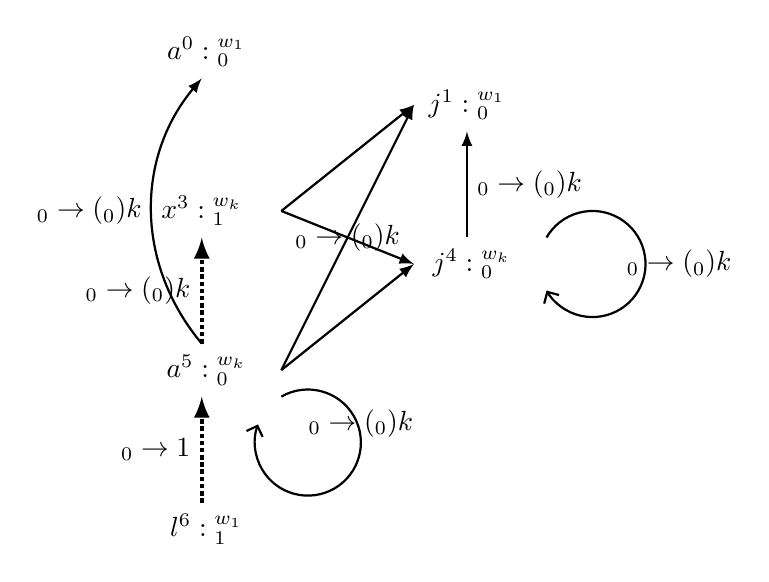
\begin{tikzpicture}[scale=\textwidth/18cm,samples=200]
\draw[] (0, 10) circle (0pt) node
{{ $a^0: {}^{w_1}_{0}$}};
\draw[] (0, 7) circle (0pt) node
{\textbf{$x^3: {}^{w_k}_{1}$}};
\draw[] (0, 4) circle (0pt) node
{{ $a^5: {}^{w_k}_{0}$}};
\draw[] (0, 1) circle (0pt) node
{{ $l^6: {}^{w_1}_{1}$}};
% Counter Variables
\draw[] (5, 9) circle (0pt) node {\textbf{$j^1: {}^{w_1}_{0}$}};
\draw[] (5, 6) circle (0pt) node {{ $j^4: {}^{w_k}_{0}$}};
%
% Value Dependency Edges:
\draw[ ultra thick, -latex, densely dotted,] (0, 1.5)  -- 
% The Weight for this edge
node [left] {\highlight{$\trace_0 \to 1 $}}(0, 3.5) ;
\draw[ ultra thick, -latex, densely dotted,] (0, 4.5)  -- 
node [left] {\highlight{$\trace_0 \to \env(\trace_0) k $}}(0, 6.5) ;
\draw[ thick, -latex] (0, 4.5)  to  [out=-230,in=230]  
node [left] {\highlight{$\trace_0 \to \env(\trace_0) k $}}(0, 9.5) ;
\draw[ thick, -Straight Barb] (1.5, 3.5) arc (120:-200:1);
    % The Weight for this edge
    \draw[](3, 3) node [] {\highlight{$\trace_0 \to \env(\trace_0) k  $}};
\draw[ thick, -Straight Barb] (6.5, 6.5) arc (150:-150:1);
    % The Weight for this edge
    \draw[](9, 6) node [] {\highlight{$\trace_0 \to \env(\trace_0) k  $}};
\draw[ thick, -latex] (5, 6.5)  -- 
% The Weight for this edge
node [right] {\highlight{$\trace_0 \to \env(\trace_0) k $}} (5, 8.5) ;
% Control Dependency
\draw[ thick,-latex] (1.5, 7)  -- (4, 9) ;
\draw[ thick,-latex] (1.5, 4)  -- 
% The Weight for this edge
node [] {\highlight{$\trace_0 \to \env(\trace_0) k $}} (4, 9) ;
\draw[ thick,-latex] (1.5, 7)  -- (4, 6) ;
\draw[ thick,-latex] (1.5, 4)  -- (4, 6) ;
\end{tikzpicture}
\caption{}
\end{centering}
\end{subfigure}
 \caption{(a) The program $\kw{towRounds(k)}$, an example 
%  of a program 
with two rounds of adaptivity (b) The corresponding execution-based dependency graph.}
\label{fig:twoRounds_example}
\end{figure}
}
\end{example}
%

% In terms of techniques, our work relies on ideas from both static analysis and dynamic analysis. 
We discuss closely related work in both areas.


%
% \subsection{Implementation}
% \label{subsec:dynamic-implementation}
%
\cleardoublepage

\chapter{The Program Static Analysis for Adaptivity}
\label{ch:adapt-algo}


\section{Introduction}
\label{sec:static-intro}

\section{Static Data Dependency Analysis}
\label{sec:static-datadep}

\section{Static Reachability Bound Analysis}
\label{sec:static-reachability}

\section{Static Adaptivity Analysis}
\label{sec:static-adapt}

\section{Examples}
\label{sec:static-examples}
%
\section{Implementation}
\label{sec:static-implementation}

\section{Related Work}
\label{sec:static-relatedwork}
In terms of techniques, our work relies on ideas from both static analysis and dynamic analysis. 
We discuss closely related work in both areas.


\cleardoublepage


% In terms of techniques, our work relies on ideas from both static analysis and dynamic analysis. 
We discuss closely related work in both areas.



% \cleardoublepage

% I review the works on studying the quantitative properties in this dissertation in the next part, 
and the future directions are also discussed. 
% \cleardoublepage

In this chapter, I conclude this dissertation, mainly studying two adaptivity of data analysis programs.


In the execution-based analysis, I will formalize the intuitive notion of \emph{adaptivity} as a quantitative 
   property of programs. This analysis is developed in three steps through different methodologies in each step. 
   \\
	a. The dependency relation between every query, through the methodology of semantic data dependency analysis.
   \\
	b. The dependency quantity analysis, through the methodology of execution-based data reachability bound analysis.
   \\
	c. The adaptivity analysis, based on the two analysis results above, give the formal \emph{adaptivity} model 
   for program.
   \\   
   % I will focus on research on how to define the Adaptivity semantically. 
   % (the Trace, Event, the Dependency relation, Dependency depth in terms of the evaluation times and the Adaptivity)
	In the static-based program analysis, I will design a static program analysis for soundly approximating this quantity.
   In this static program analysis, the program will be analysed in the same 3 aspects as the execution-based analysis 
   while through static program analysis techniques, and a sound estimated result will be given in each aspect as follows.
   \\
	a. The data dependency relation analysis through the static data flow analysis technique.
   \\
	b. The dependency quantity analysis through the static program reachability bound analysis techniques.
   \\
	c. The program adaptivity estimation, through newly designed algorithms based on the results estimated above, 
   computing the adaptivity upper bound soundly 
   and accurately.
   \\
I implement my program analysis and show that it can help to analyze the adaptivity of several concrete data analyses with different adaptivity structures.

Then, through two observations as follows,
\\
1. traditional program's resource cost analysis they failed to consider the case where the program's cost could decrease 
 implicitly, 
 \\
 2. and 
 % when there isn't a dependency relation between variables.
 the resource consumption during the program 
 execution increases and particularly decreases implicitly in the same way as the program's adaptivity, 
 % Specifically, in line 5 
 % where the list is re-written and the heap consumption is decreased implicitly. 
 % This implicit decrease 
 % of the cost works exactly the same as program's adaptivity decrease.
 I'm interested in improving the accuracy of program's general resource cost analysis
 by generalizing my \emph{adaptivity} analysis framework.
 %  onto the program's resource cost analysis. 
 % Use this framework,
 Through the generalized \emph{adaptivity} analysis framework.
 I will give
 a more accurate resource cost estimation by taking the program's implicit resource cost into consideration, comparing 
 to the worst case cost analysis in traditional way.
 For this work, the analysis framework design is expected to be done with the implementation start off before final defense.


 Finally, based on the study on traditional way of performing data flow and control analysis,
 I identify the similarity between the traditional way of performing data flow and control analysis, and the 
 adaptivity analysis.  
 Specifically I identify the similarity between 
 solving the feasible path problem in the analysis by reducing to CFL-reachability problems,
 and the way of computing the adaptivity in my static analysis framework.
 Motivated by this observation, 
 % I'm insterested
 % the, There are similarity between
 % solving the data flow problem by reducing to CFL-reachability problem,
 % resource analysis through reducing to CFL-reachability problem, 
 I'm interested in showing that
 CFL-reachability problems can be solved by reducing it into my adaptivity analysis framework. 
 This work is planed to start off before final defense and develop further sophisticated after.
\cleardoublepage


%%%%%%%%%%%%%%%%%%%%%%%%%%%%%%%%%%%%%%%%%%%%%%%%%%%%%%%%%%%%%%%%%%
% Quick references for some R packages used that I want in the bibliography
\nocite{tikzDevice,plotly,reshape,Rcomputing,Florida2000}

%%%%%%%%%%%%%%%%%%%%%%%%%%%%%%%%%%%%%%%%%%%%%%%%%%%%%%%%%%%%%%%%%%
% Put your appendices inside here, to maintain figure and table listings. Make sure to use \section{appendixA} to have some numbering for figures and tables.



\appendix
% \begin{appendices}
\begingroup
  \hypersetup{linkbordercolor=white,linkcolor=black,
    filecolor=black, urlcolor=black} 
% \addcontentsline{toc}{chapter}{List of Figures in Appendix}
\listofappendixfigures
\endgroup
% \stoplist[main]{lof}% stops main list of figures
% \startlist[appendix]{lof}
% \printlist[appendix]{lof}{}{\chapter*{List of Figures in Appendix}}
% % \chapter*{Glossary of Terms}
\label{glossary}
\begin{longtable}{r p{0.6\textwidth}}
    \textbf{\textit{Complicated Term}}: & Make sure to define anything that you allude to in the text\\
    \textbf{\textit{Parameter}}: & Description of the parameter. This is not the same as the List of Symbols. \\
\end{longtable}
\section{Implementation}
\label{appendix:implementation}
\subsection{The Implementation Evaluation Results }
\label{sec:adapt-impleval}

\jl{
We implemented $\THESYSTEM$ as a tool which takes a labeled command as input  
and outputs two upper bounds on the program adaptivity and the number of query requests respectively.
This implementation consists of an 
abstract control flow graph generation,
edge estimation (as presented in Section~\ref{sec:alg_edgegen}), and weight estimation (as presented in Section~\ref{sec:alg_weightgen}) in Ocaml, 
and the adaptivity computation algorithm shown in Section~\ref{sec:alg_adaptcompute} in Python.
The OCaml program takes the labeled command as input and outputs the program-based dependency graph and
the abstract transition graph,
feeds into the python program and the python program provides the adaptivity upper bound and the query number as the final output.
}

We evaluated this implementation on $23$ example programs with the evaluation results shown in Table~\ref{tb:adapt-imp}.
In this table,
the first column is the name of each program.
For each program $c$, the second column is its intuitive adaptivity rounds,
% the third column is the adaptivity $A(c)(\trace_0)$ w.r.t the input initial trace $\trace_0 \in \mathcal{T}_0(c)$ as definition~\ref{def:trace_adapt}.
% In all these examples, the input variable $k$ specifies the loop iteration numbers.
% Since $A(c)(\trace_0)$ by definition~\ref{def:trace_adapt} will count the execution times of
% query request command in the loop, which is indeed same as  the loop iteration numbers,
% we use $\env(\trace_0) k$ in the third column represent this number, which computes the $k$'s initial value from input initial trace $\trace_0$.
the third column is the output of the $\THESYSTEM$ implementation, which consists of two expressions.
The first one is the upper bound for adaptivity and the second one is the 
upper bound for the total number of query requests in the program. And the last column is the performance evaluation w.r.t. the program size.

\jl{
The last column is the performance evaluation.
The time contains three parts. The first part is the running time of the Ocaml code, which parses the program and generates the $\progG(c)$.
The second and third parts are the running times of the reachability bound analysis algorithm
and the adaptivity computation algorithm, $\pathsearch(c)$.
}

    The first $5$ programs are adapted from real world data analysis algorithms.
    The first two programs $\kw{twoRounds(k)}$, $ \kw{multiRounds(k)}$ are the same as Figure~\ref{fig:twoRounds}(a) and Figure~\ref{fig:multipleRounds}(a).
    $\THESYSTEM$ computes tight adaptivity bound for the first 3.
For the forth program $\kw{multiRoundsO(k)}$, $\THESYSTEM$ outputs an over-approximated upper bound $1 + 2*k$ for the $A(c)$, which is consistent with our expectation as discussed in Example~\ref{ex:multiRoundsO}. 
The fifth program is the evaluation results for the example in Example~\ref{ex:multiRoundsS}, where $\THESYSTEM$ outputs the tight bound for $A(c)$ but $A(c)$ is a loose definition of the program's actual adaptivity rounds.
%

The programs from Tab.~\ref{tb:adapt-imp} line:6-17 all have small size but complex structures, to test the programs under different situations including
data, control dependency,
the multiple paths nested loop with related counters, etc.
Both implementations compute the tight bound for examples in line:6-14
and over-approximate the adaptivities for $15^{th}$ and $16^{th}$ due to path-insensitivity.
For the $17^{th}$ one, implementation I gives tight bound bound while II gives loose bound, so we keep both implementations.

The last six programs are composed of some programs above in order to test the performance limitation when the input program is large. 
From the evaluation results, the performance bottleneck is the reachability bound analysis algorithm.
By implementing the bound analysis algorithm in Section~\ref{sec:alg_weightgen} (adapted from \cite{sinn2017complexity}), we are unable to evaluate the $\kw{Jumbo}$ in a reasonable time period.
Alternatively, we implement another light reachability bound analysis algorithm and compute the \emph{adaptivity} for
$\kw{jumboS}, \kw{jumbo}$ and $\kw{big}$ effectively.

Overall for these examples, our system gives both the accurate adaptivity definition and estimated
adaptivity upper bound through our formalization and analysis framework $\THESYSTEM$.
The complete programs are defined below from Example~\ref{ex:twoRoundsComplete} to Example~\ref{ex:nestedWhileMPRV} in the Appendix~\ref{apdx:evaluated_examples}.

{\footnotesize
\begin {table}[H]
\vspace{-0.4cm}
    \caption{Experimental results of {\THESYSTEM} implementation}
    \vspace{-0.5cm}
        \label{tb:adapt-imp}
        \begin{center}
        \centering
{\scriptsize
        \begin{tabular}{ >{\tiny}r | l | c | c | >{\tiny}c | >{\tiny}c | >{\tiny}c | >{\tiny}c  }
        \multirow{3}{*}{Program $c$} & 
        \multirow{3}{*}{\emph{adaptivity}}
         & \multicolumn{2}{c|}{$\THESYSTEM$}
         & \multicolumn{4}{c}{performance} \\ 
         \cline{3-8}
         & & \multirow{2}{*}{$\pathsearch(c)$ (I | II) } & \multirow{2}{*}{$\query$\# (I | II) } & \multirow{2}{*}{lines} & \multicolumn{3}{c}{running time (second)} \\ 
         \cline{6-8}
         & & & &  & Ocaml & Weight & $\pathsearch$  \\
         \hline \hline
         $  \kw{twoRounds(k)}$ & $2$ &  $2| -$ & $k+1 | -$  & 8 & 0.0005 & 0.0017 | 0.0002 & 0.0003 \\
         $  \kw{multiRounds(k)}$ & $k$ &  $k| \max(1,k)$ & $k| -$  &  10 & 0.0012 & 0.0017 | 0.0002 & 0.0002 \\
         $  \kw{lRGD(k, r)}$ & $k$ & $k | \max(1,k) $ & $ 2k | -$  &  10 & 0.0015 & 0.0072 | 0.0002 & 0.0002  \\
         $  \kw{mROdd(k)}$ & $1 + k$ &  $2+\max(1,2k) | - $ & $1 + 3 k | - $  &  10 & 0.0015 & 0.0061 | 0.0002 & 0.0002 \\
         $  \kw{mRSingle(k)}$    & $2$ &  $1+ \max(1, k) | -$ & $1 + k | 1 + k$  &  9 & 0.0011 & 0.0075 | 0.0002 & 0.0002 \\
        %  $  \kw{seq()}$ & $4$ & $4$ & $4$ & 4 & 0.0016 & 0.0002 & 0.0001 \\ 
        %  $  \kw{seqRV()}$ & $4$ & $4$ &  $4$ & 4 & 0.0011 & 0.0003 & 0.0001 \\  
        %  $  \kw{ifVD()}$ & $3$ & $3$ &  $3$ & 5 & 0.0010 & 0.0005  & 0.0001 \\
         $  \kw{ifCD()}$ & $3$ & $3 | 4$ &   $3| 4$  & 5 & 0.0005 & 0.0003 | 0.0001  & 0.0001 \\
         $  \kw{while(k)}$ & $1+k/2$ &   $1 +\max(1, k/2) |- $  &  $1+k/2 | - $ & 7 & 0.0021 & 0.0015| 0.0001 &  0.0001 \\
         $  \kw{whileRV(k)}$ & $1 + 2k$ &  $1 + 2k| 1 + \max(1,2k)$ & $2 + 3 k| -$  &  9 & 0.0016 & 0.0056| 0.0002 & 0.0001  \\
         $  {\kw{whileVCD(k)}} $ & ${1 + 2Q_m}$ &  ${Q+\max(1,2Q_m)}$ | - & $2+2Q_m$ | -  &  6 & 0.0016 & 0.0007 |0.0002 & 0.0001 \\
         $ {\kw{whileMPVCD(k)}}$ & $2+Q_m$ &  $2 + Q_m$ | - & $2+2Q_m$ | -  &   9 & 0.0017 & 0.0043 | 0.0002 & 0.0001 \\
         $  \kw{nestWhileVD(k)}$ & $2 + k^2$ &   $3 + k^2| -$ & $1 + k + k^2|- $   &  10 & 0.0018 & 0.0126 | 0.0002 & 0.0001  \\
         $  \kw{nestWhileRV(k)}$ & $1 + k +  k^2$ &  
         $ 2 + k +  k^2 | -$ 
         &  $2 + k + k^2| -$   &  10 & 0.0017 & 0.0186 | 0.0002 & 0.0001  \\
         $  \kw{nestWhileMV(k)}$ & $1 + 2k $ & $1 + \max(1,2k) | -$ &  $1 + k + k^2 |-$  & 10 & 0.0016 & 0.0071 | 0.0002 & 0.0001 \\
         $ \kw{nestWhileMPRV(k)}$ & $1 + k + k^2$ &  $3 + k + k^2  | -$ &  $2 + 2k + k^2 | - $  &  10 & 0.019 & 0.0999 | 0.0002 & 0.0002 \\
         \highlight{$ \kw{whileM(k)}$} & $1 + k$ &  $ 2 + \max(1,2k) | -$ & $1 + 3k | - $  &  9 & 0.0017 & 0.0062 | 0.0002 & 0.0001  \\
         \highlight{$ \kw{whileM2(k)}$} & $1 + k$ &  $ 2 + k | -$ & $1 + 3k | - $  &  9 & 0.0017 & 0.0062 | 0.0002 & 0.0001  \\
         \highlight{$\kw{nestWhileRC(k)}$} & $1 + 3k$ &  $1 + 3k | 2 + 3k + k^2$ &  $1 + 3k | 1 + k + k^2$  &  11 & 0.019 & 0.2669 | 0.0002 & 0.0007 \\
         $  \kw{mRComplete(k, N)}$ & $k$ & $ k | -  $ & $k |-$   &  27 & 0.0026 & 85.9017 | 0.0003 & 0.0004 \\
        $  \kw{mRCompose(k)}$ & $2k$ & $  2k | -$ & $ 2k | -$   &  46 & 0.0036 & 5104 | 0.0003 &  0.0013\\
         $  \kw{seqCompose(k)}$ & $12$ & $12  $ | - & $326 | -$  &  502 & 0.0426  & 1.2743 | 0.0003 & 0.0223 \\
         $  \kw{tRCompose(k)}$ & $2$ &  $ * | 2$ & $* | 1 + 5k + 2 k^2 $  &  42 & 0.0026 & * | 0.0003 & 0.0005\\
         $  \kw{{jumboS(k)}}$ & $ \max(20, 8+k^2)$ &  $ * | \max(20, 6+k+k^2)$   &   $* | {44+k+k^2} $  &  71 & 0.0035 & *| 0.0003 &  0.0085 \\
         $  \kw{jumbo(k)}$ & $ \max(20, 10+k+k^2 )$ &   $* | \max(20, 12 + k+ k^2)$  &  $* |286+26k+10k^2$   &  502 & 0.0691 & * | 0.0009 & 0.018 \\
         $  {\kw{big(k)}} $ & $22+k+k*k$ &  $* |28 + k + k^2 $ &  $* |121+11k+4k^2 $  &  214 & 0.0175 & * | 0.0004 & 0.002 
        \end{tabular}
}
\end{center}
\end{table}
}

 \subsection{More Discussions on The Evaluated Examples}  
 \subsubsection{The Complete Two Rounds Adaptive Data Analysis Algorithm, $\kw{tRComplete}$} 
 
\begin{example}[Complete Two Rounds Algorithm]
    \label{ex:twoRoundsComplete}

Below is the complete \emph{two rounds analyst strategy} for random data algorithm. This is instantiated from the
\emph{Custom Adaptive Analyst Strategy}, the Algorithm 5 in \cite{RogersRSSTW20} by setting the adaptive queries indices parameter, $S$ as the last column $\{ k \}$.

\begin{algorithm}
    \caption{The complete \emph{two rounds analyst strategy} for random data}
    \label{alg:twoRound}
    \begin{algorithmic}
    \REQUIRE Mechanism $\mathcal{M}$ with a hidden data set $D \in \{-1,+1\}^{n\times (k+1)} \subset \dbdom$.
    \STATE  {\bf for}\ $j\in [k]$\ {\bf do}.  
    \STATE \qquad {\bf define} $q_j(d)=d(j)\cdot d(k)$ where $d \in \{D(i) ~|~ i = 0, \cdots, n\} \subseteq \{-1,+1\}^{k+1}$.
    \STATE \qquad {\bf let} $a_j=\mathcal{M}(q_j)$ 
    \STATE \qquad \COMMENT{In the line above, $\mathcal{M}$ computes approx. the exp. value  of $q_j$ over $D$. So, $a_j\in [-1,+1]$.}
    \STATE {\bf define} $q_{k}(d)= d(k) \cdot \kw{sign}\big (\sum_{i\in [k]} x(i) \cdot \ln\frac{1+a_i}{1-a_i} \big )$ where $x\in \{-1,+1\}^{k+1}$.
    \STATE\COMMENT{In the line above,  $\kw{sign}(y)=\left \{ \begin{array}{lr} +1 & \kw{if}\ y\geq 0\\ -1 &\kw{otherwise} \end{array} \right . $.}
    \STATE {\bf let} $a_{k+1}=\mathcal{M}(q_{k+1})$
    \STATE\COMMENT{In the line above,  $\mathcal{M}$ computes approx. the exp. value  of $q_{k+1}$ over $X$. So, $a_{k+1}\in [-1,+1]$.}
    \RETURN $a_{k+1}$.
    \ENSURE $a_{k+1}\in [-1,+1]$
    \end{algorithmic}
    \end{algorithm}
    %
%
We also have the complete implementation of the algorithm above in our language below.
\[
    \kw{twoRounds(k)} \triangleq
\begin{array}{l}
       \clabel{ a \leftarrow []}^{1} ; \\
        \clabel{\assign{j}{k} }^{2} ; \\
        \ewhile ~ \clabel{j > 0}^{3} ~ \edo ~ \\
        \Big(
         \clabel{\assign{x}{\query(\chi[k - j]\cdot \chi[k])} }^{4}  ; \\
         \clabel{\assign{j}{j-1}}^{5} ;\\
        \clabel{a \leftarrow x :: a}^{6}       \Big);\\
        \clabel{l \leftarrow (\kw{sign}\big (\sum_{i\in [k]} \chi[i]\times\ln\frac{1+a[i]}{1-a[i]} \big ))}^{7}\\
    \end{array}
\]
%
The evaluation table in Tab.~\ref{tb:adapt-imp} shows that our {\THESYSTEM} works well for this complete implementation.
    \end{example}
 %
 \subsubsection{The Complete Multiple Rounds Adaptive Data Analysis Algorithm, $\kw{mRComplete}$} 
 
    \begin{example}[Complete Multiple Round Algorithm]
    %
    \begin{algorithm}
    \footnotesize
    \caption{A multi-round analyst strategy for random data base \cite{dwork2015generalization}}
    \label{alg:multiRound}
    \begin{algorithmic}
    \REQUIRE Mechanism $\mathcal{M}$ with a hidden state $X\in [N]^{n}$ sampled u.a.r., control set size $c$
    \STATE Define control dataset $C = \{0,1, \cdots, c - 1\}$
    \STATE Initialize $Nscore(i) = 0$ for $i \in [N]$, $I = \emptyset$ and $Cscore(C(i)) = 0$ for $i \in [c]$
    \STATE  {\bf for}\ $j\in [k]$\ {\bf do} 
    \STATE \qquad {\bf let} $p=\uniform(0,1)$ 
    \STATE \qquad {\bf define} $q (x) = \bernoulli ( p )$ .
    \STATE \qquad {\bf define} $qc (x) = \bernoulli ( p )$ .
    \STATE \qquad {\bf let} $a = \mathcal{M}(q)$ 
    \STATE \qquad {\bf for}\ $i \in [N]$\ {\bf do}
    \STATE \qquad \qquad $Nscore(i) = Nscore(i) + (a - p)*(q (i) - p)$ if $i \notin I$
    \STATE \qquad {\bf for}\ $i \in [c]$\ {\bf do}
    \STATE \qquad \qquad $Cscore(C(i)) = Cscore(C(i)) + (a - p)*(qc (i) - p)$
    \STATE \qquad {\bf let} $I = \{i | i\in [N] \land Nscore(i) > \max(Cscore)\}$
    \STATE \qquad {\bf let} $D = D \setminus I$ 
    \RETURN $D$.
    \end{algorithmic}
    \end{algorithm}
    %
    {\small
    \begin{figure}
        \begin{subfigure}{0.8\textwidth}
        \begin{centering}
        $
    \kw{multiRounds(k, c, N)} \triangleq
    \begin{array}{l}
        \clabel{\assign{j}{N}}^0 ; 
         \clabel{\assign{cs}{0}}^1; 
         \clabel{\assign{ns}{0}}^2;
         \clabel{\assign{I}{0}}^3; 
         \clabel{\assign{w}{k}}^{4} ;\\
         \ewhile ~ \clabel{j > 0}^{5} ~ \edo ~ \\
         \Big(
         \clabel{\assign{j}{j-1}}^{6} ;
         \clabel{\assign{cs}{0 + cs}}^7; 
         \clabel{\assign{ns}{0 + ns}}^8
         \Big); \\
    
         \ewhile ~ \clabel{w > 0}^{9} ~ \edo ~ \\
        \Big(
        \clabel{\assign{w}{w-1}}^{10} ;
        \left[p \leftarrow c \right]^{11}; 
        \left[q \leftarrow c \right]^{12}; 
        \left[ a \leftarrow \query (\chi[I]) \right]^{13};\\
        \clabel{\assign{i}{N}}^{14} ; 
        \ewhile ~ \clabel{i > 0}^{15} ~ \edo ~ \\
        \Big(
        \clabel{\assign{i}{i-1}}^{16} ;
        \clabel{\assign{cs(i)}{cs(i) + (a - p) * (q - p)}}^{17}; \\
        \eif (\clabel{ I < i}^{18}, \clabel{\assign{ns(i)}{{ns(i) + (a - p) * (q - p)}}}^{19},
        \clabel{\assign{ns}{ns(i)}}^{20}    )
        \Big); \\
        \clabel{\assign{i2}{N}}^{21} ; \\
        \ewhile ~ \clabel{i2 > 0}^{22} ~ \edo ~ \\
        \Big(
        \clabel{\assign{i2}{i2-1}}^{23} ;
        \eif (\clabel{ns(i2) > \kw{max}(cs)}^{24}, 
        \clabel{\assign{I}{i + I}}^{25},
        \clabel{\assign{I}{I}}^{26})
        \Big)
        \Big) 
    \end{array}
       $
       \caption{}
        \end{centering}
        \end{subfigure}
        \vspace{-0.3cm}
        \caption{(a) The labeled program implementing the multiple round algorithm (b)The same program in the SSA version}
        \vspace{-0.5cm}
        \label{fig:multiround_complete}
        \end{figure}
    }
    %
    \end{example}
 %
% \subsubsection{$\kw{lRGD}$}
% %
\begin{example}[Linear Regression Algorithm with Gradient Decent Optimization]
\label{ex:linearregression}
    The linear regression algorithm with gradient decent Optimization works well 
    in our $\THESYSTEM$ as well.
            %   \[
            %   %
            %   \begin{array}{l}
            %   \kw{linearRegression(step, rate)} \triangleq \\
            %          \clabel{ a \leftarrow 0}^{0} ; \\
            %          \clabel{ c \leftarrow 0}^{1} ; \\
            %           \clabel{\assign{j}{\kw{step}} }^{2} ; \\
            %         %   \clabel{\assign{d}{10000000} }^{2} ; \\
            %           \ewhile ~ \clabel{j > 0}^{3} ~ \edo ~ \\
            %           \Big(
            %               \clabel{\assign{da}{\query(-2 * (\chi[1] - (\chi[0]\times a + c)) \times (\chi[0]))} }^{4}  ; \\
            %               \clabel{\assign{dc}{\query(-2 * (\chi[1] - (\chi[0]\times a + c)))} }^{5}  ; \\
            %               \clabel{\assign{a}{a - \kw{rate} * da} }^{6}  ; \\
            %               \clabel{\assign{c}{c - \kw{rate} * dc} }^{7}  ; \\
            %            \clabel{\assign{j}{j-1}}^{8} 
            %         %   \clabel{a \leftarrow x :: a}^{6} 
            %           \Big);
            %       \end{array}
            %   \]
              %
              %
                   %
\begin{figure}
\centering
\begin{subfigure}{0.45\textwidth}
    \centering
    {\small
        \[
        \begin{array}{l}
            \kw{linearRegressionGD(k, rate)} \triangleq \\
                   \clabel{ a \leftarrow 0}^{0} ; 
                   \clabel{ c \leftarrow 0}^{1} ; 
                    \clabel{\assign{j}{\kw{k}} }^{2} ; \\
                  %   \clabel{\assign{d}{10000000} }^{2} ; \\
                    \ewhile ~ \clabel{j > 0}^{3} ~ \edo ~ \\
                    \Big(
                        \clabel{\assign{da}{\query(-2 * (\chi[1] - (\chi[0]\times a + c)) \times (\chi[0]))} }^{4}  ; \\
                        \clabel{\assign{dc}{\query(-2 * (\chi[1] - (\chi[0]\times a + c)))} }^{5}  ; \\
                        \clabel{\assign{a}{a - \kw{rate} * da} }^{6}  ; 
                        \clabel{\assign{c}{c - \kw{rate} * dc} }^{7}  ; \\
                     \clabel{\assign{j}{j-1}}^{8} 
                  %   \clabel{a \leftarrow x :: a}^{6} 
                    \Big);
                \end{array}
        \]
        }
     \caption{}
        \end{subfigure}
        \begin{subfigure}{.5\textwidth}
            \begin{centering}
            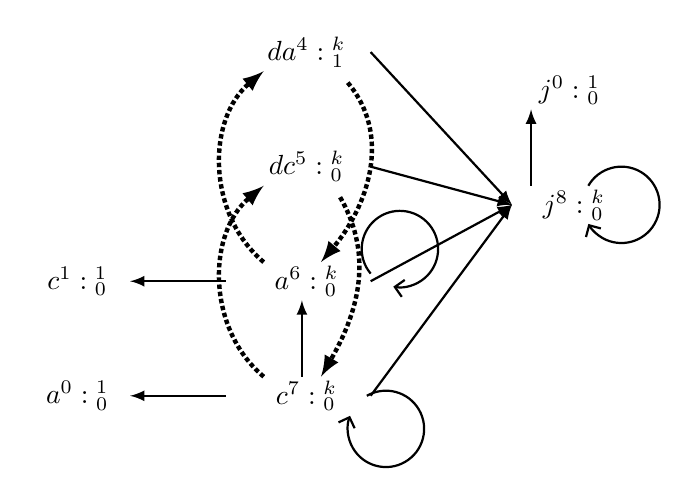
\begin{tikzpicture}[scale=\textwidth/25cm,samples=200]
    % Variables Initialization
    \draw[] (-6, 1) circle (0pt) node{{ $a^0: {}^1_{0}$}};
    \draw[] (-6, 4) circle (0pt) node{{ $c^1: {}^{1}_{0}$}};
    % Variables Inside the Loop
         \draw[] (0, 10) circle (0pt) node{{ $da^4: {}^{k}_{1}$}};
         \draw[] (0, 7) circle (0pt) node{{ $dc^5: {}^{k}_{0}$}};
         \draw[] (0, 4) circle (0pt) node{{ $a^6: {}^{k}_{0}$}};
         \draw[] (0, 1) circle (0pt) node{{ $c^7: {}^{k}_{0}$}};
         % Counter Variables
         \draw[] (7, 9) circle (0pt) node {{$j^0: {}^{1}_{0}$}};
         \draw[] (7, 6) circle (0pt) node {{ $j^8: {}^{k}_{0}$}};
         %
         % Value Dependency Edges:
         \draw[ thick, -latex,] (0, 1.5)  -- (0, 3.5) ;
         \draw[ thick, -Straight Barb] (1.8, 4.2) arc (220:-100:1);
         \draw[ thick, -Straight Barb] (7.5, 6.5) arc (150:-150:1);
         \draw[ thick, -latex] (6, 6.5)  -- (6, 8.5) ;
         \draw[ thick, -Straight Barb] (1.7, 1.) arc (120:-200:1);
         % Value Dependency Edges on Initial Values:
         \draw[ thick, -latex,] (-2, 1)  -- (-4.5, 1) ;
         \draw[ thick, -latex,] (-2, 4)  -- (-4.5, 4) ;
         %
         \draw[ ultra thick, -latex, densely dotted,] (-1, 1.5)  to  [out=-220,in=220]  (-1, 6.5);
         \draw[ ultra thick, -latex, densely dotted,] (-1, 4.5)  to  [out=-220,in=220]  (-1, 9.5);
         \draw[ ultra thick, -latex, densely dotted,]  (1, 6.2) to  [out=-60,in=60] (0.5, 1.5) ;
         \draw[ ultra thick, -latex, densely dotted,]  (1.2, 9.2)  to  [out=-50,in=50] (0.5, 4.5);
         % Control Dependency
        %  \draw[ thick,-latex] (1.5, 7)  -- (4, 9) ;
        %  \draw[ thick,-latex] (1.5, 4)  -- (4, 9) ;
         \draw[ thick,-latex] (1.8, 7)  -- (5.5, 6) ;
         \draw[ thick,-latex] (1.8, 4)  -- (5.5, 6) ;
         \draw[ thick,-latex] (1.8, 1)  -- (5.5, 6) ;
         \draw[ thick,-latex] (1.8, 10)  -- (5.5, 6) ;
         \end{tikzpicture}
         \caption{}
            \end{centering}
            \end{subfigure}
    \vspace{-0.5cm}
    \caption{(a) The linear regression algorithm 
    (b) The program-based dependency graph from $\THESYSTEM$}
    \vspace{-0.5cm}
    \label{fig:linear_regression}
\end{figure}
%
Analysis Result: $ \progA(\kw{linearRegressionGD(k, rate)}) = k$
\end{example} 
%
 
This linear regression algorithm 
% in order to
aims to
model a linear relationship between a dependent variable $y$,
% corresponding to the observed value in the column $\chi[1]$ in database, 
and an independent variable $x$, $y = a \times x + c$, specifically approximating the 
model parameter $a$ and $c$.
In order to have a good approximation on the model parameter 
$a$ and $c$, 
% corresponding to the observed value in the column $\chi[0]$ in database, 
it sends query to a training data set adaptively in every iteration.
This training data set contains two columns (can extend to higher dimensional data sets), first column is used as the observed value for the independent variable $x$,
second column is used as the observed label value for the dependent variable $y$.
This algorithm is written in our {\tt Query While} language in Figure~\ref{fig:linear_regression}(a) as $\kw{linearRegressionGD(k, rate)}$.
% taking the iteration number $\kw{step}$ 

This linear regression algorithm starts from initializing the linear model parameters and the counter variable,
and then goes into the training iterations.
In each iteration, it computes the differential value w.r.t. parameter
$a$ and $c$ respectively,
through requesting two queries, $\query(-2 * (\chi[1] - (\chi[0]\times a + c)) \times (\chi[0]))$ and 
$\query(-2 * (\chi[1] - (\chi[0]\times a + c)))$
at line 4 and 5.
Then, it uses these two differential values stored in variable $da$ and $dc$ to update the linear model parameters $a$ and $c$.
%
Its the program-based dependency graph is shown in Figure~\ref{fig:linear_regression}(b). Its execution-based dependency graph share the same graph, only needs to change the weight, $k$ into $w_k$ and $1$ for $w_1$ as we do in the previous example.
% We omit the detail of how to 
% generate this graph, which is similar to the generation procedure in 
% Example~\ref{alg:multiRound}.
In the execution-based dependency graph, there are multiple walks having the same longest query length.
For example, the walk $c^7 \to dc^6 : \to c^7 \to \cdots \to dc^6$ along the 
dotted arrows, where each vertex is visited $w_k(\trace_0)$ times for an initial trace $\trace_0$.
% By counting the total occurrence time of vertices with annotation $1$ in this walk, we have this program's adaptivity $k$.
There is actually other walks having the same query length $k$, the 
walk $a^7 \to da^6  \to a^7 \to \cdots \to da^6 $ along the 
dotted arrows, where each vertex is visited $w_k(\trace_0)$ times.
% the dotted path corresponds to a finite walk with the longest query length and its adaptivity on this walk is $k$.
But it doesn't affect the adaptivity for this program, which is still the maximal query length $w_k(\trace_0)$ with respect to initial trace $\trace_0$.
Also, $\THESYSTEM$, estimates the adaptivity $k$ for this example. Similarly as the multiple round example, we can show it is a tight bound.
%
 %          
% \subsubsection{The Programs for Examples from line:6 - 15 in Table.\ref{tb:adapt-imp}}
% %
    \begin{example}[The Complete Gradient Decent Optimization Algorithm]
        This example is the gradient decent algorithm example is a generalization of the linear regression on a higher degree data relation.
        It uses gradient decent algorithm to minimize 
        the mean square loss function
        for a two-degree relation
         $y = a_1 \times x_1^2 + a_2 \times x_2 + c$
        on the dataset of two feature columns and one indicator column.
     \[
     %
     \begin{array}{l}
     \kw{gradientDecent(step, rate, t, n)} \triangleq \\
        \clabel{ a_1 \leftarrow 0}^{0} ; \\
        \clabel{ a_2 \leftarrow 0}^{1} ; \\
        \clabel{ c \leftarrow 0}^{2} ; \\
        \clabel{\assign{j}{\kw{step}} }^{3} ; \\
        \ewhile ~ \clabel{j > 0}^{4} ~ \edo ~ \\
      \Big(
          \clabel{\assign{da1}{\query(-2 * (\chi[2] - (\chi[0]^2 \times a_1 + \chi[1] \times a_2 + c)) \times (\chi[0]))} }^{5}  ; \\
          \clabel{\assign{da2}{\query(-2 * (\chi[2] - (\chi[0]^2 \times a_1 + \chi[1] \times a_2 + c)) \times (\chi[1]))} }^{6}  ; \\  \clabel{\assign{dc}{\query(-2 * (\chi[2] - (\chi[0]^2 \times a_1 + \chi[1] \times a_2 + c)))} }^{5}  ; \\
          \clabel{\assign{a_1}{a_1 - \kw{rate} * da1} }^{7}  ; \\
          \clabel{\assign{a_2}{a_2 - \kw{rate} * da2} }^{8}  ; \\
          \clabel{\assign{c}{c - \kw{rate} * dc} }^{9}  ; \\
       \clabel{\assign{j}{j-1}}^{10} 
      \Big);
  \end{array}
     \]
     %
     %
        This approach can be generalized to the regression of a variety of 
        relations in machine learning area.
   %
     \end{example}
%

    \begin{example}[Sequence with Linear Query Dependency]
        \label{ex:seq}
        This example algorithm contains only sequence of four query commands.
        Each of them depends on a previous query.
        The longest dependency depth, i.e., the adaptivity is expectation to be $4$.
        %
        %
        \[
        %
            \kw{seq()} \triangleq 
        \begin{array}{l} 
               \clabel{ \assign{x}{\chi[0]}}^{0} ; 
   \clabel{\assign{y}{\chi[x + 1]} }^{1} ; \\
   \clabel{\assign{z}{\chi[y + 1]}}^{2}; 
    \clabel{\assign{w}{\chi[z + 1]} }^{3}
            \end{array}
        \]
        Evaluation Result: $ \progA( \kw{seq()}) = 4$
        \end{example}
    %
    \begin{example}[Sequence with Query Dependency between Related Variables]
        \label{ex:seqRV}
        %
        This example algorithm contains a sequence of four query commands.
        Each of them depends on one or more of the previous queries.
        The longest dependency depth, i.e., the adaptivity is expectation to be $4$.
        %
        \[
        %
            \kw{seqRV()} \triangleq 
        \begin{array}{l} 
               \clabel{ \assign{x}{\chi[0]}}^{0} ;
   \clabel{\assign{y}{\chi[x + 1]} }^{1} ; \\
   \clabel{\assign{z}{\chi[y + x]}}^{2}; 
    \clabel{\assign{w}{\chi[z + 1] \cdot \chi[y]} }^{3}
            \end{array}
        \]
        Evaluation Result: $ \progA(\kw{seqMultiVar()}) = 4$
    \end{example}
    %
        \begin{example}[If with Data-Value Dependency Separated]
            \label{ex:ifVD}
            This example algorithm contains a $\eif$ command and a query requests
            in each branch.
            Only the query in the first branch depend on the query in the command $0$,
            and the variable in the guard is not assigned by a query request.
            % Each of them depends on one or more of the previous queries.   %
            The longest dependency depth, i.e., the adaptivity is expectation to be $3$.
            \[
            %
            \kw{ifVD}(k) \triangleq 
            \begin{array}{l}
               \quad \clabel{ \assign{z}{\query(\chi[0])}}^{0} ; 
               \quad \clabel{\assign{x}{k / 2} }^{1} ; \\
               \quad \eif(\clabel{x < 0}^2,
               \quad \clabel{\assign{y}{\query(\chi[z])}}^{3},
               \quad \clabel{\assign{y}{\query(\chi[0])}}^{4})
   \end{array}
            \]
            Evaluation Result: $ \progA( \kw{ifVD()}) = 3$
        \end{example}
    
            \begin{example}[If with Data-Control Dependency Overlapped]
   \label{ex:ifCD}
   %
   This example algorithm contains a $\eif$ command and a query requests
   in each branch.
   The variable in the guard is assigned by a query request in command $1$.
   The two queries in the branches depend on the second query in command $1$
   but not depend on the query in the command $0$.
   Even though the variable $x$ isn't used in the query expression in the query $3$ and $4$,
   there are still dependency relation because $x$ is in the guard.
%
The longest dependency depth, i.e., the adaptivity is expectation to be $3$.
   \[
   %
   \kw{ifCD()} \triangleq 
   \begin{array}{l}
\clabel{ \assign{z}{\query(\chi[0])}}^{0} ;
\clabel{\assign{x}{\query(\chi[z])} }^{1} ; \\
\eif(\clabel{x < 0}^{2}, 
\clabel{\assign{y}{\query(\chi[0] + \chi[1])}}^{3}, 
\clabel{\assign{y}\query{(\chi[0])}}^{4})
   \end{array}
   \]
   %
   Evaluation Result: $ \progA( \kw{ifCD()}) = 3$
   \end{example}
    
    
\begin{example}[While with Nested Query Dependency]
\label{ex:whileNested}
This example algorithm contains a simple while loop.
There is one query requests in the loop body at command $3$.
In each iteration, the query request depend on the query result from previous iteration.
The longest dependency depth, i.e., the adaptivity is expectation to be $k$.
%
\[
%
\kw{whileNested}(k) \triangleq
\begin{array}{l}
    \clabel{ \assign{j}{k} }^{0} ; 
    \clabel{ \assign{a}{\query(\chi[0])} }^{1} ; \\
        \ewhile ~ \clabel{j > 0}^{2} ~ \edo ~ \\
        \Big(
         \clabel{\assign{x}{\query(\chi[a]) }}^{3}  ; 
         \clabel{\assign{a}{x + a}}^{4} ;
        \clabel{\assign{j}{j-1}}^{5}       \Big)
    \end{array}
\]
The Evaluation Result: $ \progA(\kw{whileRec}(k)) = 1 + k$
   \end{example}
    %
            \begin{example}[While with Multi-Path Query Dependency]
   \label{ex:whileM}
   %
   This example algorithm contains a simple while loop and a $\eif$ command in the loop body.
% There is one query requests in the loop body at command $3$.
Each branch  has a query request (in the commands $5$ and $6$)
depend on the query at command $1$ and the query at command $7$.
Among the $\frac{k}{2}$ iterations,
% the query at command $7$ depend on the query at line $5$, otherwise not.
 result from previous iteration.
The longest dependency depth, i.e., the adaptivity is expectation to be $1 +2 * \lfloor \frac{k}{2} \rfloor$.
            %
            \[
            %
            \kw{whileM}(k) \triangleq 
            \begin{array}{l}
   \clabel{ \assign{j}{k}}^{0} ; 
   \clabel{ \assign{x}{\query(\chi[0])} }^{1} ; \\
\ewhile ~ \clabel{j > 0}^{2} ~ \edo ~ \\
\Big(
 \clabel{\assign{j}{j-1}}^{3} ;\\
 \eif(\clabel{j \% 2 == 0}^{4}, 
 \clabel{\assign{y}{\chi[x]}}^{5}, 
 \clabel{\assign{w}{\chi[x]}}^{6});\\        
 \clabel{\assign{x}{\query(\chi(\ln(y)))} }^{7} \Big)
   \end{array}
            \]
            The Evaluation Result: $ \progA(\kw{whileM}(k)) = 1 +2 * \lfloor \frac{k}{2} \rfloor $
        \end{example}
    %
            \begin{example}[While with Query Dependency through Related Variables]
   \label{ex:whileRV}
   This example algorithm contains a simple while loop
    and a sequence of three query requests in the loop body.
% There is one query requests in the loop body at command $3$.
In each iteration, every query request depend on one or more
query results from previous iteration.
% the query at command $7$ depend on the query at line $5$, otherwise not.
The longest dependency depth, i.e., the adaptivity is expectation to be $1 +2 * k$.
   \[
   %
   \kw{whileRV}(k) \triangleq 
   \begin{array}{l}
   \clabel{\assign{j}{k} }^{0} ; 
   \clabel{ \assign{x}{\query(\chi[0])}}^{1} ; 
\clabel{ \assign{y}{\query(\chi[1])}}^{2} ; \\
    \ewhile ~ \clabel{j > 0}^{3} ~ \edo ~ \\
    \Big(
     \clabel{\assign{j}{j-1}}^{4} ;
     \clabel{\assign{z}{\query(\chi(x + \ln(y)))} }^{5}  ; 
     \clabel{ \assign{x}{\query(\chi[z])}}^{6} ; 
     \clabel{ \assign{y}{\query(\chi[z])}}^{7} 
    \Big)
\end{array}
   \]
   The Evaluation Result: $ \progA(\kw{whileRV}(k)) = 1 + 2 * k $
            \end{example}
   %
   %
   \begin{example}[While with Query Dependency trhough Control Flow and Data Flow]
\label{ex:whileVCD}
%
This example algorithm contains a simple while loop
and a sequence of three query requests in the loop body.
The variable in the guard is assigned by a query request in command $0$.
In each iteration, the query at $3$ depends on either the query at line $1$, and the query result at line $4$ from the previous iteration.
%  in the branches depend on the second query in command $1$
In each iteration, the query at $4$ depends on either the query at line $0$ and the query at line $3$ in the same iteration.
% Even though the variable $x$ isn't used in the query expression in the query $3$ and $4$,
The longest dependency depth, i.e., the adaptivity is expectation to be $1 +2 * k$.
\[
\kw{whileVCD}() \triangleq
\begin{array}{l}
    \clabel{ \assign{x}{\query(\chi[0])} }^{0} ; 
    \clabel{ \assign{z}{\query(\chi[0])} }^{1} ; \\
        \ewhile ~ \clabel{x > 0}^{2} ~ \edo ~ \\
        \Big(
        \clabel{\assign{x}{\query(\chi(z))} }^{3}  ; 
        \clabel{\assign{z}{\query(\chi(x))}}^{4}
      \Big)
    \end{array}
\]
The Evaluation Result: $ \progA(\kw{whileVCD}(k)) = 1 + 2 * k $
   \end{example}
    %
   \begin{example}[While with Multiple Path Query Dependency Dependency]
\label{ex:whileMPVCD}
%
This example algorithm contains a simple while loop and a $\eif$ command in the loop body.
% There is one query requests in the loop body at command $3$.
Each branch  has a query request (in the commands $5$ and $6$)
depend on either the query at command $1$ or the query at command $7$.
% Among the $\frac{k}{2}$ iterations,
% % the query at command $7$ depend on the query at line $5$, otherwise not.
%  result from previous iteration.
The longest dependency depth, i.e., the adaptivity is expectation to be $2 + k$.
\[
    %
    \kw{whileMPVCD}(k) \triangleq
    \begin{array}{l}
        \clabel{ \assign{x}{\query(k)}}^{0} ; 
        \clabel{\assign{y}{0} }^{1} ; 
            \ewhile ~ \clabel{x > 0}^{2} ~ \edo ~ \\
            \Big(
             \eif(\clabel{y > 0}^{3}, 
             \clabel{\assign{y}{\query(\chi[12])}}^{4}, 
             \clabel{\assign{w}{\query(\chi[9])}}^{5});        
             \\
             \clabel{\assign{x}{x-1}}^{6}\Big);\\
             \clabel{\assign{y}{\query(\chi(\ln(y)))} }^{7} 
        \end{array}
    \]
    The Evaluation Result: $ \progA(\kw{whileMPVCD}(k)) = 2 + k $
\end{example}
   %
\begin{example}[Nested While with Nested Query Dependency]
    \label{ex:nestWhileVD}
    %
    This example algorithm contains two nested while loops.
    The query in the outer loop at line $5$ depends on either the query at line $1$ or
    the query results at line $8$ from the previous iteration of the inner loop.
    The longest dependency depth, i.e., the adaptivity is expectation to be $2 + k^2$.
        %
    \[
    %
    \kw{nestWhileVD}(k) \triangleq 
    \begin{array}{l}
        \clabel{ \assign{i}{k} }^{0} ; 
        \clabel{\assign{x}{\query(\chi[0])}}^{1} ; \\
            \ewhile ~ \clabel{i > 0}^{2} ~ \edo ~ 
            \Big(
             \clabel{\assign{i}{i-1}}^{3} ;
             \clabel{\assign{j}{k}}^{4} ;
             \clabel{\assign{y}{\query(\chi(\ln(x)))} }^{5}  ; \\
             \ewhile ~ \clabel{j > 0}^{6} ~ \edo ~ 
             \Big(
              \clabel{\assign{j}{j-1}}^{7};
              \clabel{\assign{x}{\query(\chi(\ln(x)))} }^{8}
              \Big) \Big)
        \end{array}
    \]
    The Evaluation Result: $ \progA(\kw{nestWhileVD}(k)) = 2 + k^2 $
\end{example}
    
    \begin{example}[Nested While with Query Dependency through Related Variables]
        \label{ex:nestedWhileRV}
        %
        This example algorithm contains two nested while loops, one query in the outer loop, and one query in the inner loop.
        The query in the outer loop at line $8$ depends on only the query result at line $7$
        from the last iteration of the inner loop.
        %  either the query at line $1$ or
        However, the query at line $7$ depends on  either the query at line $1$ 
        the query results at line $8$ from the previous iteration.
        The longest dependency depth, i.e., the adaptivity is expectation to be $1 + 2 * k $.
            %
        \[
        %
            \kw{nestWhileRV}(k) \triangleq 
        \begin{array}{l}
            \clabel{ \assign{i}{k} }^{0} ; 
            \clabel{\assign{x}{\query(\chi[0])}}^{1} ; \\
   \ewhile ~ \clabel{i > 0}^{2} ~ \edo ~ 
   \Big(
    \clabel{\assign{i}{i-1}}^{3} ;
    \clabel{\assign{j}{k}}^{4} ;\\
    \ewhile ~ \clabel{j > 0}^{5} ~ \edo ~ 
    \Big(
     \clabel{\assign{j}{j-1}}^{6};
     \clabel{\assign{y}{\query(\chi(x) + \chi(1))} }^{7}
     \Big); \\
    \clabel{\assign{x}{\query(\chi(\ln(y)))} }^{8}
     \Big)
            \end{array}
        \]
        The Evaluation Result: $ \progA(\kw{nestWhileRV}(k)) = 1 + 2 * k $
    \end{example}
%
   
        \begin{example}[Nested While with Nest Query Dependency and Related Variable Accross Outer and Inner Loop]
            \label{ex:nestedWhileMR}
            %
            This example algorithm contains two nested while loops, one query in the outer loop, and one query in the inner loop as well.
            The two queries depend on both the query results assigned to themselves in previous iteration.
            The longest dependency depth, i.e., the adaptivity is expectation to be $1 + k + k^2 $.
            \[
            %
            \kw{nestWhileMR}(k) \triangleq 
            \begin{array}{l}
                \clabel{\assign{i}{k} }^{0} ; 
                \clabel{ \assign{x}{\query(\chi[0])}}^{1} ; 
                \clabel{ \assign{y}{\query(\chi[1])}}^{2} ; 
                \ewhile ~ \clabel{i > 0}^{3} ~ \edo ~ \\
                \Big(
                \clabel{\assign{i}{i-1}}^{4} ;
                \clabel{\assign{j}{k}}^{5} ;
                \clabel{\assign{y}{\query(\chi(\ln(x) + y))} }^{6}  ; \\
                \ewhile ~ \clabel{j > 0}^{7} ~ \edo ~ 
                \Big(
                \clabel{\assign{j}{j-1}}^{8};
                \clabel{\assign{x}{\query(\chi(\ln(y))+\chi[x])} }^{9}
                \Big) \Big)
            \end{array}
            \]
            The Evaluation Result: 
            $ \progA(\kw{nestWhileMR}(k)) = 1 + k + k^2$
            \\
            Reachability Bound The Evaluation Result: \\
            weight for Variable: j of label 6 is: 0 + 0 + 1 * k * k\\
            weight for Variable: y of label 7 is: 0 + 0 + 1 * k * k\\
            weight for Variable: j of label 4 is: 0 + 1 * k\\
            weight for Variable: i of label 3 is: 0 + 1 * k\\
            weight for Variable: x of label 8 is: 0 + 1 * k\\
            weight for Variable: x of label 1 is: 1\\
            weight for Variable: i of label 0 is: 1\\
            \end{example}
            \begin{example}[Nested While with MultiplePath and Nested Recursive Multiple Variable 
   Data-Value Dependency Across Outer and Inner Loop]
   \label{ex:nestedWhileMPRV}
   %
   We then show a more complex example with nested while command and nested data-flow across the outer and inner while loop through multiple variables.
   This example also contains the if command with data dependency occurred through the if guard.
   The longest dependency depth, i.e., the adaptivity is expectation to be $1 + k + k^2 $.
   %
   \[
   %
   \kw{nestWhileMPRV}(k) \triangleq 
   \begin{array}{l}
\clabel{\assign{i}{k} }^{0} ; 
\clabel{ \assign{x}{\query(\chi[0])}}^{1} ; 
\clabel{ \assign{y}{\query(\chi[1])}}^{2} ; \\
    \ewhile ~ \clabel{i > 0}^{3} ~ \edo ~ 
    \Big(
     \clabel{\assign{i}{i-1}}^{4} ;
     \clabel{\assign{j}{k}}^{5} ;\\
     \eif(\clabel{x > 0}^6, \clabel{\assign{y}{\query(\chi(\ln(x) + y))} }^{7},
     \clabel{\assign{y}{\query(\chi(x))} }^{8} )
      ; \\
     \ewhile ~ \clabel{j > 0}^{9} ~ \edo ~ 
     \Big(
      \clabel{\assign{j}{j-1}}^{10};
      \clabel{\assign{x}{\query(\chi(\ln(y))+\chi[x])} }^{11}
      \Big) \Big)
\end{array}
   \]
   \end{example}
   The Evaluation Result: $ \progA(\kw{nestWhileMPRV}(k)) = 1 + k + k^2$
   \\
   Reachability Bound The Evaluation Result: \\
            weight for Variable: j of label 10 is: 0 + 0 + 1 * k * k \\
   weight for Variable: x of label 11 is: 0 + 0 + 1 * k * k \\
   weight for Variable: y of label 7 is: 0 + 1 * k \\
   weight for Variable: y of label 8 is: 0 + 1 * k \\
   weight for Variable: j of label 5 is: 0 + 1 * k \\
   weight for Variable: i of label 4 is: 0 + 1 * k \\
   weight for Variable: y of label 2 is: 1 \\
   weight for Variable: x of label 1 is: 1 \\
   weight for Variable: i of label 0 is: 1 \\

% \subsubsection{The Programs for Examples from line:16 - 20 in Table.\ref{tb:adapt-imp}}
% \begin{example}[$\kw{mRCompose}$]
The composed multiple rounds program:
\\
\lstinputlisting[language=Python]{codes/mRcompose.br}
\end{example}
\begin{example}[$\kw{tRCompose}$]
The composed two rounds program:
\\
\lstinputlisting[language=Python]{codes/trCompose.br}
\end{example}
\begin{example}[$\kw{seqCompose}$]
    The composed two rounds program:
    \\
    \lstinputlisting[language=Python]{codes/seqCompose.br}
\end{example}
\begin{example}[$\kw{jumboS}$]
    The composed program with nested loops. 
    \\
    \lstinputlisting[language=Python]{codes/jumboS.br}
\end{example}
\begin{example}[$\kw{jumbo}$]
    The composed program with multiple paths nested loops. 
    \\
    \lstinputlisting[language=Python]{codes/jumbo.br}
\end{example}


\section{Soundness of Path In-Sensitive Reachability Bounds Analysis}
\label{apdx:reachability_soundness}
  \begin{thm}[Soundness of the Reachability Bounds Estimation]
    \label{thm:vertexweight_soundness}
  Given a program ${c}$ with its program-based dependency graph 
  $\progG(c) = (\progV, \progE)$,
  % $\traceG = (\traceV, \traceE, \traceW, \traceF)$, 
  we have:
    %
    \[
      \begin{array}{l}
        \forall c \in \cdom 
        % , (v, n) \in \mathcal{VAR} \times \mathbb{N} \times \mathbb{N}
         \sthat  
        %  \\ \quad
         \progG({c}) = (\progV, \progE)
        \land 
        \traceG({c}) = (\traceV, \traceE)
        \\ \quad
        \implies
        \forall (x^l, w_{t}) \in \traceV,
        (x^l, w_{p}) \in \progV, 
        \trace_0 \in \mathcal{T}_0(c), 
        \trace' \in \mathcal{T}, v \in \mathbb{N} \sthat 
        \\ \quad
        \config{{c}, \trace_0} \to^{*} \config{\eskip, \trace_0\tracecat\vtrace'} 
        \land 
        \config{w^{p}, \trace_0} \earrow v
        \implies
        % \right\} 
        w_{t}(\trace) \leq v
      \end{array}
      \]
  \end{thm}
%
\begin{proof}
  Taking an arbitrary a program ${c}$ with its program-based dependency graph 
  $\progG(c) = (\progV, \progE)$, 
  and an arbitrary pair of labeled variable and weights $(x^l, w) \in \progV$, 
  and arbitrary $\vtrace, \trace' \in \mathbb{T},
  v \in \mathbb{N}$ satisfying
  \\
  % \max \left\{ 
    % \vcounter(\vtrace') l ~ \middle\vert~
  % \forall \vtrace, \trace' \in \mathcal{T} \sthat  
  $\config{{c}, \trace} \to^{*} \config{\eskip, \trace\tracecat\vtrace'} 
  \land 
  \config{\trace, w} \earrow v$
  %  labelled variable $x^l \in \lvar_c$.
  \\
  By Definition of $\progV$ in $\progG(c)$, we know 
  $  w = \absW(l) = \max \{ \absclr(\absevent) | \absevent = (l, \_, \_)\}$.
  \\
  By Lemma~\ref{lem:abscfg_sound}, there exists an abstract event in $\absflow(c)$ of form $(\absevent) = (l, \_, \_)$,
  corresponding to the assignment command associated to labeled variable $x^l$. 
  \\
  Let $(\absevent) = (l, dc, l') \in \absflow(c)$ be this event for some $dc$ and $l'$ such that  $(\absevent) = (l, dc, l') \in \absflow(c)$,
  by the last step of phase 2, we know
  $
  \progW(x^l) 
  \triangleq \absclr(\absevent)
  $.
   Then, it is sufficient to show:
  \[
  %   \max \left\{ \vcounter(\vtrace') l ~ \middle\vert~
  % \forall \vtrace \in \mathcal{T} \sthat  \config{{c}, \trace} \to^{*} \config{\eskip, \trace\tracecat\vtrace'} \right\} 
  % \leq 
  \forall v \in \mathbb{N} \sthat  
  \config{\absclr(\absevent), \trace} \earrow 
  \vcounter(\vtrace', l) \leq v
  \absclr(\absevent)
  \]
  % By line:2 of Algorithm~\ref{alg:add_weights}, there are 2 cases:
  By definition of $\absclr(\absevent)$:
  \[
 \begin{array}{ll}
  \locbound(\absevent) & \locbound(\absevent) \in \constdom \\
  Incr(\locbound(\absevent)) + 
  \sum\{\absclr(\absevent') \times \max(\varinvar(a) + c, 0) | (\absevent', a, c) \in \reset(\locbound(\absevent))\} 
  & \locbound(\absevent) \notin \constdom
\end{array}
\]
  \caseL{$\locbound(\absevent) \in \constdom$}
  \\
  Proved by the soundness of Local bound in Lemma~\ref{lem:local_bound_sound}.
  \caseL{$\locbound(\absevent) \notin \constdom$}
To show:
\[
  \begin{array}{l}
    \max \left\{ \vcounter(\vtrace') l ~ \middle\vert~
\forall \vtrace \in \mathcal{T} \sthat  \config{{c}, \trace} \to^{*} \config{\eskip, \trace\tracecat\vtrace'} \right\} 
\\
\leq 
Incr(\locbound(\absevent)) + 
\sum\{\absclr(\absevent') \times \max(\varinvar(a) + c, 0) | (\absevent', a, c) \in \reset(\locbound(\absevent))\} 
\end{array}
\]
  % \caseL{$l \in prel$}
  % \\
  Taking an arbitrary initial trace
  $\trace_0 \in \mathcal{T}$, 
  executing $c$ with $\trace_0$, let $\trace$ be the trace after evaluation, i.e., $\config{{c}, \trace_0} \to^{*} \config{\eskip,\vtrace}$, it is sufficient to show:
  \[ 
    \begin{array}{l}
      \vcounter(\vtrace') l \leq 
    Incr(\locbound(\absevent)) + 
    \sum\{\absclr(\absevent') \times \max(\varinvar(a) + c, 0) | (\absevent', a, c) \in \reset(\locbound(\absevent))\}
  \end{array}
  \]
%
 By the soundness of the (1) Transition Bound and (2) Variable Bound Invariant 
 in \cite{sinn2017complexity} Theorem 1, 
This case is proved.
\end{proof}
% \begin{lem}[Soundness of the Abstract Execution Trace]
%   \label{lem:abscfg_sound}
% Given a program ${c}$, we have:
% %
% \[
%   \begin{array}{l}
%     \forall \vtrace_0, \trace \in \mathcal{T} ,  \event = (\_, l, \_) \in \eventset \sthat 
% \config{{c}, \trace_0} \to^{*} \config{\eskip, \trace_0 \tracecat \vtrace} 
% \land \event \in \trace 
% \\
% \qquad \implies \exists \absevent = (l, \_, \_) \in Label(c) \times Label(c) \times \absdom \sthat  
% \absevent \in \absflow(c)
% \end{array}
% \]
% \end{lem}
\begin{lem}[Soundness of the Abstract Execution Trace]
  \label{lem:abscfg_sound}
Given a program ${c}$, we have:
%
\[
  \begin{array}{l}
    \forall \vtrace_0, \trace \in \mathcal{T} ,  \event = (\_, l, \_) \in \eventset \sthat 
\config{{c}, \trace_0} \to^{*} \config{\eskip, \trace_0 \tracecat \vtrace} 
\land \event \in \trace 
\\
\qquad \implies \exists \absevent = (l, \_, \_) \in (\ldom\times \dcdom^{\top} \times \ldom) \sthat  
\absevent \in \absflow(c)
\end{array}
\]
\end{lem}
%    This lemma is proved formally in Appendix~\ref{apdx:reachability_soundness}.
% For every event $\event$ with label $l$ in an execution trace $\trace$ of program $c$, 
% there is an abstract event in program's abstract execution trace of form $(l, \_, \_)$. 
% This lemma is proved formally in Lemma~\ref{lem:abscfg_sound} in Appendix~\ref{apdx:reachability_soundness}.
% \\
\begin{proof}
  Taking arbitrary $\trace_0 \in \mathcal{T}$, and an arbitrary event $\event = (\_, l, \_) \in \eventset$, it is sufficient to show:
  \[
  \begin{array}{l}
    \forall \trace \in \mathcal{T} \sthat 
\config{{c}, \trace_0} \to^{*} \config{\eskip, \trace_0 \tracecat \vtrace} 
\land \event \in \trace 
\\
\qquad \implies 
% \exists \absevent = (l, \_, \_) \in Label(c) \times Label(c) \times \absdom \sthat  
% \absevent \in \absflow(c)
\exists \absevent = (l, \_, \_) \in (\ldom\times \dcdom^{\top} \times \ldom) \sthat  
\absevent \in \absflow(c)
\end{array}
\]
  By induction on program $c$, we have the following cases:
  \caseL{$c = [\assign{x}{\expr}]^{l'}$}
  By the evaluation rule $\rname{assn}$, we have
  $
  {
  \config{[\assign{{x}}{\aexpr}]^{l'},  \trace } 
  \xrightarrow{} 
  \config{\eskip, \trace \tracecat [({x}, l', v) ]}
  }$, for some $v \in \mathbb{N}$ and $\trace = [({x}, l', v) ]$.
  \\
  There are 2 cases, where $l' = l$ and $l' \neq l$.
  \\
  In case of $l' \neq l$, we know $\event \not\eventin \trace$, then this Lemma is vacuously true.
    \\
    In case of $l' = l$, by the abstract Execution Trace computation, we know 
    $\absflow(c) = \absflow'([x := \expr]^{l}; \clabel{\eskip}^{l_e}) = \{(l, \absexpr(\expr), l_e)\}$  
    \\
  Then we have $\absevent = (l, \absexpr(\expr), l_e) $ and $\absevent \in \absflow(c)$.
  \\
  This case is proved.
  \caseL{$c = [\assign{x}{\query(\qexpr)}]^{l'}$}
  This case is proved in the same way as \textbf{case: $c = [\assign{x}{\expr}]^l$}.
  \caseL{$\ewhile [b]^{l_w} \edo c$}
  If the rule applied to is $\rname{while-t}$, we have
  \\
  $\config{{\ewhile [b]^{l_w} \edo c_w, \trace}}
    \xrightarrow{} 
    \config{{
    c_w; \ewhile [b]^{l_w} \edo c_w,
    \trace_0 \tracecat [(b, l, \etrue)]}}
  $.
  \\
  Let $\trace_w \in \mathcal{T}$ satisfying following execution:
  \\
  $
  \config{{
  c_w,
  \trace_0 \tracecat [(b, l_w, \etrue)]}}
  \xrightarrow{*} 
  \config{{
  \eskip,
  \trace_0 \tracecat [(b, l_w, \etrue)] \tracecat \trace_w}}
$
\\
Then we have the following execution:
\\
$\config{{\ewhile [b]^{l_w} \edo c_w, \trace}}
\xrightarrow{} 
\config{{
c_w; \ewhile [b]^{l_w} \edo c_w,
\trace_0 \tracecat [(b, l_w, \etrue)]}}
\xrightarrow{*} 
\config{{
  \ewhile [b]^{l_w} \edo c_w,
\trace_0 \tracecat [(b, l_w, \etrue)] \tracecat \trace_w}}
\xrightarrow{*} 
\config{{
\eskip,
\trace_0 \tracecat [(b, l_w, \etrue)] \tracecat \trace_w \tracecat \trace_1}}
$ for some $\trace_1 \in \mathcal{T}$ and $\trace = [(b, l_w, \etrue)] \tracecat \trace_w \tracecat \trace_1$.
\\
Then we have 3 cases: 
(1) $\event \eventeq (b, l_w, \etrue)$, 
(2) $\event \in \trace_w$ or 
(3) $\event \in \trace_1$.
  \\
In case of (1). $\event \eventeq (b, l_w, \etrue)$, since $\absflow(c) = \absflow'(c;\clabel{\eskip}^{l_e}) = \{(l, \top, \init(c_w))\} \cup \cdots $, we have $\absevent = (l, \top, \init(c_w))$ and this case is proved.
\\
In case of (2). $\event \in \trace_w$,
by induction hypothesis on 
$c_w$ with the execution 
  $\config{{
  c_w,
  \trace_0 \tracecat [(b, l_w, \etrue)]}}
  \xrightarrow{*} 
  \config{{
  \eskip,
  \trace_0 \tracecat [(b, l_w, \etrue)] \tracecat \trace_w}}$ and trace $\trace_w$, 
  we know there is an abstract event of the form 
  $\absevent' = (l, \_, \_ ) \in \absflow(c_w)$ where $\absflow(c_w) = \absflow'(c_w;\clabel{\eskip}^{l_e})$.
  \\
  Let $\absevent' = (l, dc, l')$ for some $dc$ and $l'$ such that $\absevent \in \absflow(c)$.
  \\
  By definition of $\absflow'$, we have 
  $ \absflow'(c_w;\clabel{\eskip}^{l_e}) = 
  \absflow'(c_w) \cup  \{ (l', dc, l_e) | (l', dc) \in \absfinal(c_w) \} $.
  \\
  There are 2 subcases: (2.1) $\absevent' \in \absflow'(c_w)$ or 
  $ (2.2) \absevent' \in \{ (l', dc, l_e) | (l', dc) \in \absfinal(c_w) \}$.
  \subcaseL{(2.1)}
  Since $\absflow(c) = \absflow'(c_w) \cup \{(l', dc, l_w)| (l', dc) \in \absfinal(c_w) \} \cup \cdots $, 
  we know the abstract event $\absevent' \in \absflow(c)$. 
  \\
  This case is proved.
  \subcaseL{(2.2) $\absevent' \in \{ (l', dc, l_e) | (l', dc) \in \absfinal(c_w) \}$ }
  In this case, we know $(l, dc) \in \absfinal(c_w)$.
  \\
  Since $\absflow(c) = \absflow'(c_w) \cup \{(l', dc, l_w)| (l', dc) \in \absfinal(c_w) \} \cup \cdots $, 
  we know $(l, dc, l_w) \in \{(l', dc, l_w)| (l', dc) \in \absfinal(c_w) \}$, 
   i.e., the abstract event $(l, dc, l_w) \in \absflow(c)$ and $(l, dc, l_w)$ has the form $(l, \_, \_)$.
  \\
  This case is proved.
  \\
  %
In case of (3). $\event \in \trace_1$, we know either $\event = (b, l_w, \_)$, or $\event \in \trace_w'$ where $\trace_w' \in \mathcal{T}$ is the trace of executing $c_w$ in an iteration.
\\
Then this case is proved by repeating the proof in case (1) and case (2).
  % And we also have the existence of $l = l_b, b$ and $c_w$, and $\ewhile [b]^{l} \edo c_w \in_c c_2$ and  $c_1 \in c_w$.
  % \\
  % If $c_w$ isn't a sequence command, let $c_1 = c_w$, then we have $c_2 = \ewhile [b]^{l} \edo c_w,  \eskip)$ 
  % and $c_1 \in_c c_2$.
  % \\
  % And we also have the existence of $l = l_b, b$ and $c_w$, and $\ewhile [b]^{l} \edo c_w \in_c c_2$ and  $c_1 \in c_w$.
  % \\
  \\
  If the rule applied to is $\rname{while-f}$, we have
  \\
  $
  {
    \config{{\ewhile [b]^{l_w} \edo c_w, \trace_0}}
    \xrightarrow{}^\rname{while-f}
    \config{{
    \eskip,
    \trace_0 \tracecat [(b, l_w, \efalse)]}}
  }$,
  In this case, we have $\trace = [(b, l_w, \efalse)]$ and $\event = (b, l_w, \efalse)$ (o.w., $\event \not\eventin \trace$ and this lemma is vacuously true) with $l = l_w$.
  \\
  By the abstract execution trace computation, $\absflow(c) = \{(l, \top, \init(c_w))\} \cup \cdots $, 
  we have $\absevent = (l, \top, \init(c_w))$  and $\absevent \in \absflow(c)$.
\\
  This case is proved.
  \caseL{$\eif([b]^l, c_t, c_f)$}
  This case is proved in the same way as \textbf{case: $c = \ewhile [b]^{l} \edo c$}.
  \caseL{$c = c_{s1};c_{s2}$}
 By the induction hypothesis on $c_{s1}$ and $c_{s2}$ separately, and the same step as case (2). of \textbf{case: $c = \ewhile [b]^{l} \edo c$},
 we have this case proved.
\end{proof}

\begin{lem}[Soundness of the Local Bound]
  \label{lem:local_bound_sound}
Given a program ${c}$, we have:
%
\[
\forall \absevent = (l, dc, l') \sthat  
\max \left\{ \vcounter(\vtrace') l ~ \middle\vert~
\forall \vtrace \in \mathcal{T} \sthat  \config{{c}, \trace} \to^{*} \config{\eskip, \trace\tracecat\vtrace'} \right\} 
\leq 
\locbound(\absevent)
\]
\end{lem}
\begin{proof}
  \subcaseL{$l \notin SCC(\absG(c))$}
  In this case, we know variable $x^l$ isn't involved in the body of any $\ewhile$ command. 
  \\
  Taking an arbitrary $\vtrace_0 \in \mathcal{T}$, 
  let $\trace \in \mathcal{T}$ be of resulting trace of executing $c$ with $\trace$, 
  i.e., $\config{{c}, \trace_0} \to^{*} \config{\eskip, \trace}$,
  \\
  we know the
  assignment command at line $l$ associated with the abstract event $\absevent$ will be executed at most once, i.e.,:
  %
  $\vcounter(\vtrace) l \leq 1$
  \\
  By $\locbound$ definition, we know $\locbound(\absevent) = 1$.
  \\
  This case is proved.
  \subcaseL{$l \in SCC(\absG(c)) \land \absevent \in \dec(x) $}  in this case, we know $\locbound(\absevent) \triangleq x$.
  \subcaseL{$l \in SCC(\absG(c)) \land \absevent 
  \notin \bigcup_{x \in VAR} \dec(x)
  \land \absevent \notin SCC(\absG(c)/\dec(x)) $}  in this case, we know $\locbound(\absevent) \triangleq x$.
  \\
  In the two cases above, the soundness is discussed in \cite{sinn2017complexity} Section 4 of Paragraph \emph{Discussion on Soundness} in Page 25.
\end{proof}

% \begin{lem}[Soundness of the Variable Bound Invariant]
%   \label{lem:var_invariant_soundness}
% Given a program ${c}$, we have:
% %
% \[
% \forall x^l \in \lvar_c \sthat  
% \max \left\{ \vcounter(\vtrace') l ~ \middle\vert~
% \forall \vtrace \in \mathcal{T} \sthat  \config{{c}, \trace} \to^{*} \config{\eskip, \trace\tracecat\vtrace'} \right\} 
% \leq 
% \rb(x^l, c)
% \]
% \end{lem}

% \begin{lem}[Soundness of the Transition Clousre ]
%   \label{lem:transition_closure_soundness}
% Given a program ${c}$, we have:
% %
% \[
% \forall x^l \in \lvar_c \sthat  
% \max \left\{ \vcounter(\vtrace') l ~ \middle\vert~
% \forall \vtrace \in \mathcal{T} \sthat  \config{{c}, \trace} \to^{*} \config{\eskip, \trace\tracecat\vtrace'} \right\} 
% \leq 
% \rb(x^l, c)
% \]
% \end{lem}

%   {
%   \begin{lem}[Soundness of the Reachability Analysis]
%     \label{lem:reachability_soundness}
%   Given a program ${c}$, we have:
%   %
%   \[
%   \forall x^l \in \lvar_c \sthat  
%   \max \left\{ \vcounter(\vtrace') l ~ \middle\vert~
%   \forall \vtrace \in \mathcal{T} \sthat  \config{{c}, \trace} \to^{*} \config{\eskip, \trace\tracecat\vtrace'} \right\} 
%   \leq 
%   \rb(x^l, c)
%   \]
%   \end{lem}
% }
% Proof Summary:
% \\
% 1. Translating of each command estimate the upper bound of the change of each variable showing up in the guard of the while command, in each iteration.
% \\
% 2. Composition of sequence either preserve the latest update of the variable, or compose it with variables flows to it.
% \\
% 3. Composition of if preserve the variable upper bound in both of the 2 branches.
% \\
% 4. Composition of a nested $\ewhile$ multiples the variable change upper bound by the bound of the nested while loop, which safely estimated the variable upper bound for the outside while loop.
% \\
% 5. Ranking function matches the pattern for every possibility and Give the max upper bound of changes for variable showing up inside the guard of the while.
% \\
% 6. By estimating the changes for all the variables in the boolean expression of the guard of the while in 1 iteration, computeBound divides the n by the changes of the boolean expression is the safe upper bound of how many times this while can looped. 
%
% \begin{lem}[Uniqueness of the Abstract Event]
%   \label{lem:absevent_unique}
% Given a program ${c}$, we have:
% %
% \[
%   \begin{array}{l}
%     \forall x^l \in \lvar_c \sthat 
% \exists \absevent = (l, \_, \_) \in Label(c) \times Label(c) \times \absdom \sthat  
% \absevent \in \absflow(c)
% \end{array}
% \]
% \end{lem}
For every labeled variable in program $c$, $x^l \in \lvar_c$, there is a unique abstract event in program's abstract execution trace $\absevent \in \absflow(c)$ of form $(l, \_, \_)$. 
\begin{lem}[Uniqueness of the Abstract Execution Trace]
\label{lem:absevent_unique}
Given a program ${c}$, we have:
%
\[
\begin{array}{l}
 \forall \vtrace_0, \trace \in \mathcal{T} ,  \event = (\_, l, \_, \_) \in \eventset^{\asn} \sthat 
\config{{c}, \trace_0} \to^{*} \config{\eskip, \trace_0 \tracecat \vtrace} 
\land \event \in \trace 
\\
\qquad \implies \exists! \absevent = (l, \_, \_) \in (\ldom\times \dcdom^{\top} \times \ldom) \sthat  
\absevent \in \absflow(c)
\end{array}
\]
\end{lem}
% This lemma and proof is also 
% formalized in Lemma~\ref{lem:absevent_unique} in Appendix~\ref{apdx:reachability_soundness}.
\begin{proof}
  This is proved trivially by induction on the program $c$.
\end{proof}
%
%
% \begin{lem}[Correspondance between $flow(c)$ and $\absflow(c)$]
%   \label{lem:flow_to_absflow}
% Given a program ${c}$, we have:
% %
% \[
% \forall \absevent = (l, dc, l') \sthat  
% \absevent \in \absflow(c) \land l' \neq l_e
% \implies (l, l') \in flow(c)
% \]
% \end{lem}
% \begin{proof}
%   This is proved trivially by induction on the program $c$.
% \end{proof}
\clearpage

\subsection{Soundness of Path Sensitive Reachability Bounds Estimation}
\label{apdx:ps_reachability_soundness}
  \begin{thm}[Soundness of the Reachability Bounds Estimation]
    \label{thm:vertexweight_soundness}
  Given a program ${c}$ with its program-based dependency graph 
  $\progG(c) = (\progV, \progE)$,
  % $\traceG = (\traceV, \traceE, \traceW, \traceF)$, 
  we have:
    %
    \[
      \begin{array}{l}
        \forall c \in \cdom 
        % , (v, n) \in \mathcal{VAR} \times \mathbb{N} \times \mathbb{N}
         \sthat  
        %  \\ \quad
         \progG({c}) = (\progV, \progE)
        \land 
        \traceG({c}) = (\traceV, \traceE)
        \\ \quad
        \implies
        \forall (x^l, w_{t}) \in \traceV,
        (x^l, w_{p}) \in \progV, 
        \trace_0 \in \mathcal{T}_0(c), 
        \trace' \in \mathcal{T}, v \in \mathbb{N} \sthat 
        \\ \quad
        \config{{c}, \trace_0} \to^{*} \config{\eskip, \trace_0\tracecat\vtrace'} 
        \land 
        \config{w^{p}, \trace_0} \earrow v
        \implies
        % \right\} 
        w_{t}(\trace) \leq v
      \end{array}
      \]
  \end{thm}
%
\begin{proof}
  Taking an arbitrary a program ${c}$ with its program-based dependency graph 
  $\progG(c) = (\progV, \progE)$, 
  and an arbitrary pair of labeled variable and weights $(x^l, w) \in \progV$, 
  and arbitrary $\vtrace, \trace' \in \mathbb{T},
  v \in \mathbb{N}$ satisfying
  \\
  % \max \left\{ 
    % \vcounter(\vtrace') l ~ \middle\vert~
  % \forall \vtrace, \trace' \in \mathcal{T} \sthat  
  $\config{{c}, \trace} \to^{*} \config{\eskip, \trace\tracecat\vtrace'} 
  \land 
  \config{\trace, w} \earrow v$
  %  labelled variable $x^l \in \lvar_c$.
  \\
  By Definition of $\progV$ in $\progG(c)$, we know 
  $  w = \absW(l) = \max \{ \absclr(\absevent) | \absevent = (l, \_, \_)\}$.
  \\
  By Lemma~\ref{lem:abscfg_sound}, there exists an abstract event in $\absflow(c)$ of form $(\absevent) = (l, \_, \_)$,
  corresponding to the assignment command associated to labeled variable $x^l$. 
  \\
  Let $(\absevent) = (l, dc, l') \in \absflow(c)$ be this event for some $dc$ and $l'$ such that  $(\absevent) = (l, dc, l') \in \absflow(c)$,
  by the last step of phase 2, we know
  $
  \progW(x^l) 
  \triangleq \absclr(\absevent)
  $.
   Then, it is sufficient to show:
  \[
  %   \max \left\{ \vcounter(\vtrace') l ~ \middle\vert~
  % \forall \vtrace \in \mathcal{T} \sthat  \config{{c}, \trace} \to^{*} \config{\eskip, \trace\tracecat\vtrace'} \right\} 
  % \leq 
  \forall v \in \mathbb{N} \sthat  
  \config{\absclr(\absevent), \trace} \earrow 
  \vcounter(\vtrace', l) \leq v
  \absclr(\absevent)
  \]
  % By line:2 of Algorithm~\ref{alg:add_weights}, there are 2 cases:
  By definition of $\absclr(\absevent)$:
  \[
 \begin{array}{ll}
  \locbound(\absevent) & \locbound(\absevent) \in \constdom \\
  Incr(\locbound(\absevent)) + 
  \sum\{\absclr(\absevent') \times \max(\varinvar(a) + c, 0) | (\absevent', a, c) \in \reset(\locbound(\absevent))\} 
  & \locbound(\absevent) \notin \constdom
\end{array}
\]
  \caseL{$\locbound(\absevent) \in \constdom$}
  \\
  Proved by the soundness of Local bound in Lemma~\ref{lem:local_bound_sound}.
  \caseL{$\locbound(\absevent) \notin \constdom$}
To show:
\[
  \begin{array}{l}
    \max \left\{ \vcounter(\vtrace') l ~ \middle\vert~
\forall \vtrace \in \mathcal{T} \sthat  \config{{c}, \trace} \to^{*} \config{\eskip, \trace\tracecat\vtrace'} \right\} 
\\
\leq 
Incr(\locbound(\absevent)) + 
\sum\{\absclr(\absevent') \times \max(\varinvar(a) + c, 0) | (\absevent', a, c) \in \reset(\locbound(\absevent))\} 
\end{array}
\]
  % \caseL{$l \in prel$}
  % \\
  Taking an arbitrary initial trace
  $\trace_0 \in \mathcal{T}$, 
  executing $c$ with $\trace_0$, let $\trace$ be the trace after evaluation, i.e., $\config{{c}, \trace_0} \to^{*} \config{\eskip,\vtrace}$, it is sufficient to show:
  \[ 
    \begin{array}{l}
      \vcounter(\vtrace') l \leq 
    Incr(\locbound(\absevent)) + 
    \sum\{\absclr(\absevent') \times \max(\varinvar(a) + c, 0) | (\absevent', a, c) \in \reset(\locbound(\absevent))\}
  \end{array}
  \]
%
 By the soundness of the (1) Transition Bound and (2) Variable Bound Invariant 
 in \cite{sinn2017complexity} Theorem 1, 
This case is proved.
\end{proof}
% \begin{lem}[Soundness of the Abstract Execution Trace]
%   \label{lem:abscfg_sound}
% Given a program ${c}$, we have:
% %
% \[
%   \begin{array}{l}
%     \forall \vtrace_0, \trace \in \mathcal{T} ,  \event = (\_, l, \_) \in \eventset \sthat 
% \config{{c}, \trace_0} \to^{*} \config{\eskip, \trace_0 \tracecat \vtrace} 
% \land \event \in \trace 
% \\
% \qquad \implies \exists \absevent = (l, \_, \_) \in Label(c) \times Label(c) \times \absdom \sthat  
% \absevent \in \absflow(c)
% \end{array}
% \]
% \end{lem}
\begin{lem}[Soundness of the Abstract Execution Trace]
  \label{lem:abscfg_sound}
Given a program ${c}$, we have:
%
\[
  \begin{array}{l}
    \forall \vtrace_0, \trace \in \mathcal{T} ,  \event = (\_, l, \_) \in \eventset \sthat 
\config{{c}, \trace_0} \to^{*} \config{\eskip, \trace_0 \tracecat \vtrace} 
\land \event \in \trace 
\\
\qquad \implies \exists \absevent = (l, \_, \_) \in (\ldom\times \dcdom^{\top} \times \ldom) \sthat  
\absevent \in \absflow(c)
\end{array}
\]
\end{lem}
%    This lemma is proved formally in Appendix~\ref{apdx:reachability_soundness}.
% For every event $\event$ with label $l$ in an execution trace $\trace$ of program $c$, 
% there is an abstract event in program's abstract execution trace of form $(l, \_, \_)$. 
% This lemma is proved formally in Lemma~\ref{lem:abscfg_sound} in Appendix~\ref{apdx:reachability_soundness}.
% \\
\begin{proof}
  Taking arbitrary $\trace_0 \in \mathcal{T}$, and an arbitrary event $\event = (\_, l, \_) \in \eventset$, it is sufficient to show:
  \[
  \begin{array}{l}
    \forall \trace \in \mathcal{T} \sthat 
\config{{c}, \trace_0} \to^{*} \config{\eskip, \trace_0 \tracecat \vtrace} 
\land \event \in \trace 
\\
\qquad \implies 
% \exists \absevent = (l, \_, \_) \in Label(c) \times Label(c) \times \absdom \sthat  
% \absevent \in \absflow(c)
\exists \absevent = (l, \_, \_) \in (\ldom\times \dcdom^{\top} \times \ldom) \sthat  
\absevent \in \absflow(c)
\end{array}
\]
  By induction on program $c$, we have the following cases:
  \caseL{$c = [\assign{x}{\expr}]^{l'}$}
  By the evaluation rule $\rname{assn}$, we have
  $
  {
  \config{[\assign{{x}}{\aexpr}]^{l'},  \trace } 
  \xrightarrow{} 
  \config{\eskip, \trace \tracecat [({x}, l', v) ]}
  }$, for some $v \in \mathbb{N}$ and $\trace = [({x}, l', v) ]$.
  \\
  There are 2 cases, where $l' = l$ and $l' \neq l$.
  \\
  In case of $l' \neq l$, we know $\event \not\eventin \trace$, then this Lemma is vacuously true.
    \\
    In case of $l' = l$, by the abstract Execution Trace computation, we know 
    $\absflow(c) = \absflow'([x := \expr]^{l}; \clabel{\eskip}^{l_e}) = \{(l, \absexpr(\expr), l_e)\}$  
    \\
  Then we have $\absevent = (l, \absexpr(\expr), l_e) $ and $\absevent \in \absflow(c)$.
  \\
  This case is proved.
  \caseL{$c = [\assign{x}{\query(\qexpr)}]^{l'}$}
  This case is proved in the same way as \textbf{case: $c = [\assign{x}{\expr}]^l$}.
  \caseL{$\ewhile [b]^{l_w} \edo c$}
  If the rule applied to is $\rname{while-t}$, we have
  \\
  $\config{{\ewhile [b]^{l_w} \edo c_w, \trace}}
    \xrightarrow{} 
    \config{{
    c_w; \ewhile [b]^{l_w} \edo c_w,
    \trace_0 \tracecat [(b, l, \etrue)]}}
  $.
  \\
  Let $\trace_w \in \mathcal{T}$ satisfying following execution:
  \\
  $
  \config{{
  c_w,
  \trace_0 \tracecat [(b, l_w, \etrue)]}}
  \xrightarrow{*} 
  \config{{
  \eskip,
  \trace_0 \tracecat [(b, l_w, \etrue)] \tracecat \trace_w}}
$
\\
Then we have the following execution:
\\
$\config{{\ewhile [b]^{l_w} \edo c_w, \trace}}
\xrightarrow{} 
\config{{
c_w; \ewhile [b]^{l_w} \edo c_w,
\trace_0 \tracecat [(b, l_w, \etrue)]}}
\xrightarrow{*} 
\config{{
  \ewhile [b]^{l_w} \edo c_w,
\trace_0 \tracecat [(b, l_w, \etrue)] \tracecat \trace_w}}
\xrightarrow{*} 
\config{{
\eskip,
\trace_0 \tracecat [(b, l_w, \etrue)] \tracecat \trace_w \tracecat \trace_1}}
$ for some $\trace_1 \in \mathcal{T}$ and $\trace = [(b, l_w, \etrue)] \tracecat \trace_w \tracecat \trace_1$.
\\
Then we have 3 cases: 
(1) $\event \eventeq (b, l_w, \etrue)$, 
(2) $\event \in \trace_w$ or 
(3) $\event \in \trace_1$.
  \\
In case of (1). $\event \eventeq (b, l_w, \etrue)$, since $\absflow(c) = \absflow'(c;\clabel{\eskip}^{l_e}) = \{(l, \top, \init(c_w))\} \cup \cdots $, we have $\absevent = (l, \top, \init(c_w))$ and this case is proved.
\\
In case of (2). $\event \in \trace_w$,
by induction hypothesis on 
$c_w$ with the execution 
  $\config{{
  c_w,
  \trace_0 \tracecat [(b, l_w, \etrue)]}}
  \xrightarrow{*} 
  \config{{
  \eskip,
  \trace_0 \tracecat [(b, l_w, \etrue)] \tracecat \trace_w}}$ and trace $\trace_w$, 
  we know there is an abstract event of the form 
  $\absevent' = (l, \_, \_ ) \in \absflow(c_w)$ where $\absflow(c_w) = \absflow'(c_w;\clabel{\eskip}^{l_e})$.
  \\
  Let $\absevent' = (l, dc, l')$ for some $dc$ and $l'$ such that $\absevent \in \absflow(c)$.
  \\
  By definition of $\absflow'$, we have 
  $ \absflow'(c_w;\clabel{\eskip}^{l_e}) = 
  \absflow'(c_w) \cup  \{ (l', dc, l_e) | (l', dc) \in \absfinal(c_w) \} $.
  \\
  There are 2 subcases: (2.1) $\absevent' \in \absflow'(c_w)$ or 
  $ (2.2) \absevent' \in \{ (l', dc, l_e) | (l', dc) \in \absfinal(c_w) \}$.
  \subcaseL{(2.1)}
  Since $\absflow(c) = \absflow'(c_w) \cup \{(l', dc, l_w)| (l', dc) \in \absfinal(c_w) \} \cup \cdots $, 
  we know the abstract event $\absevent' \in \absflow(c)$. 
  \\
  This case is proved.
  \subcaseL{(2.2) $\absevent' \in \{ (l', dc, l_e) | (l', dc) \in \absfinal(c_w) \}$ }
  In this case, we know $(l, dc) \in \absfinal(c_w)$.
  \\
  Since $\absflow(c) = \absflow'(c_w) \cup \{(l', dc, l_w)| (l', dc) \in \absfinal(c_w) \} \cup \cdots $, 
  we know $(l, dc, l_w) \in \{(l', dc, l_w)| (l', dc) \in \absfinal(c_w) \}$, 
   i.e., the abstract event $(l, dc, l_w) \in \absflow(c)$ and $(l, dc, l_w)$ has the form $(l, \_, \_)$.
  \\
  This case is proved.
  \\
  %
In case of (3). $\event \in \trace_1$, we know either $\event = (b, l_w, \_)$, or $\event \in \trace_w'$ where $\trace_w' \in \mathcal{T}$ is the trace of executing $c_w$ in an iteration.
\\
Then this case is proved by repeating the proof in case (1) and case (2).
  % And we also have the existence of $l = l_b, b$ and $c_w$, and $\ewhile [b]^{l} \edo c_w \in_c c_2$ and  $c_1 \in c_w$.
  % \\
  % If $c_w$ isn't a sequence command, let $c_1 = c_w$, then we have $c_2 = \ewhile [b]^{l} \edo c_w,  \eskip)$ 
  % and $c_1 \in_c c_2$.
  % \\
  % And we also have the existence of $l = l_b, b$ and $c_w$, and $\ewhile [b]^{l} \edo c_w \in_c c_2$ and  $c_1 \in c_w$.
  % \\
  \\
  If the rule applied to is $\rname{while-f}$, we have
  \\
  $
  {
    \config{{\ewhile [b]^{l_w} \edo c_w, \trace_0}}
    \xrightarrow{}^\rname{while-f}
    \config{{
    \eskip,
    \trace_0 \tracecat [(b, l_w, \efalse)]}}
  }$,
  In this case, we have $\trace = [(b, l_w, \efalse)]$ and $\event = (b, l_w, \efalse)$ (o.w., $\event \not\eventin \trace$ and this lemma is vacuously true) with $l = l_w$.
  \\
  By the abstract execution trace computation, $\absflow(c) = \{(l, \top, \init(c_w))\} \cup \cdots $, 
  we have $\absevent = (l, \top, \init(c_w))$  and $\absevent \in \absflow(c)$.
\\
  This case is proved.
  \caseL{$\eif([b]^l, c_t, c_f)$}
  This case is proved in the same way as \textbf{case: $c = \ewhile [b]^{l} \edo c$}.
  \caseL{$c = c_{s1};c_{s2}$}
 By the induction hypothesis on $c_{s1}$ and $c_{s2}$ separately, and the same step as case (2). of \textbf{case: $c = \ewhile [b]^{l} \edo c$},
 we have this case proved.
\end{proof}

\begin{lem}[Soundness of the Local Bound]
  \label{lem:local_bound_sound}
Given a program ${c}$, we have:
%
\[
\forall \absevent = (l, dc, l') \sthat  
\max \left\{ \vcounter(\vtrace') l ~ \middle\vert~
\forall \vtrace \in \mathcal{T} \sthat  \config{{c}, \trace} \to^{*} \config{\eskip, \trace\tracecat\vtrace'} \right\} 
\leq 
\locbound(\absevent)
\]
\end{lem}
\begin{proof}
  \subcaseL{$l \notin SCC(\absG(c))$}
  In this case, we know variable $x^l$ isn't involved in the body of any $\ewhile$ command. 
  \\
  Taking an arbitrary $\vtrace_0 \in \mathcal{T}$, 
  let $\trace \in \mathcal{T}$ be of resulting trace of executing $c$ with $\trace$, 
  i.e., $\config{{c}, \trace_0} \to^{*} \config{\eskip, \trace}$,
  \\
  we know the
  assignment command at line $l$ associated with the abstract event $\absevent$ will be executed at most once, i.e.,:
  %
  $\vcounter(\vtrace) l \leq 1$
  \\
  By $\locbound$ definition, we know $\locbound(\absevent) = 1$.
  \\
  This case is proved.
  \subcaseL{$l \in SCC(\absG(c)) \land \absevent \in \dec(x) $}  in this case, we know $\locbound(\absevent) \triangleq x$.
  \subcaseL{$l \in SCC(\absG(c)) \land \absevent 
  \notin \bigcup_{x \in VAR} \dec(x)
  \land \absevent \notin SCC(\absG(c)/\dec(x)) $}  in this case, we know $\locbound(\absevent) \triangleq x$.
  \\
  In the two cases above, the soundness is discussed in \cite{sinn2017complexity} Section 4 of Paragraph \emph{Discussion on Soundness} in Page 25.
\end{proof}

% \begin{lem}[Soundness of the Variable Bound Invariant]
%   \label{lem:var_invariant_soundness}
% Given a program ${c}$, we have:
% %
% \[
% \forall x^l \in \lvar_c \sthat  
% \max \left\{ \vcounter(\vtrace') l ~ \middle\vert~
% \forall \vtrace \in \mathcal{T} \sthat  \config{{c}, \trace} \to^{*} \config{\eskip, \trace\tracecat\vtrace'} \right\} 
% \leq 
% \rb(x^l, c)
% \]
% \end{lem}

% \begin{lem}[Soundness of the Transition Clousre ]
%   \label{lem:transition_closure_soundness}
% Given a program ${c}$, we have:
% %
% \[
% \forall x^l \in \lvar_c \sthat  
% \max \left\{ \vcounter(\vtrace') l ~ \middle\vert~
% \forall \vtrace \in \mathcal{T} \sthat  \config{{c}, \trace} \to^{*} \config{\eskip, \trace\tracecat\vtrace'} \right\} 
% \leq 
% \rb(x^l, c)
% \]
% \end{lem}

%   {
%   \begin{lem}[Soundness of the Reachability Analysis]
%     \label{lem:reachability_soundness}
%   Given a program ${c}$, we have:
%   %
%   \[
%   \forall x^l \in \lvar_c \sthat  
%   \max \left\{ \vcounter(\vtrace') l ~ \middle\vert~
%   \forall \vtrace \in \mathcal{T} \sthat  \config{{c}, \trace} \to^{*} \config{\eskip, \trace\tracecat\vtrace'} \right\} 
%   \leq 
%   \rb(x^l, c)
%   \]
%   \end{lem}
% }
% Proof Summary:
% \\
% 1. Translating of each command estimate the upper bound of the change of each variable showing up in the guard of the while command, in each iteration.
% \\
% 2. Composition of sequence either preserve the latest update of the variable, or compose it with variables flows to it.
% \\
% 3. Composition of if preserve the variable upper bound in both of the 2 branches.
% \\
% 4. Composition of a nested $\ewhile$ multiples the variable change upper bound by the bound of the nested while loop, which safely estimated the variable upper bound for the outside while loop.
% \\
% 5. Ranking function matches the pattern for every possibility and Give the max upper bound of changes for variable showing up inside the guard of the while.
% \\
% 6. By estimating the changes for all the variables in the boolean expression of the guard of the while in 1 iteration, computeBound divides the n by the changes of the boolean expression is the safe upper bound of how many times this while can looped. 
%
% \begin{lem}[Uniqueness of the Abstract Event]
%   \label{lem:absevent_unique}
% Given a program ${c}$, we have:
% %
% \[
%   \begin{array}{l}
%     \forall x^l \in \lvar_c \sthat 
% \exists \absevent = (l, \_, \_) \in Label(c) \times Label(c) \times \absdom \sthat  
% \absevent \in \absflow(c)
% \end{array}
% \]
% \end{lem}
For every labeled variable in program $c$, $x^l \in \lvar_c$, there is a unique abstract event in program's abstract execution trace $\absevent \in \absflow(c)$ of form $(l, \_, \_)$. 
\begin{lem}[Uniqueness of the Abstract Execution Trace]
\label{lem:absevent_unique}
Given a program ${c}$, we have:
%
\[
\begin{array}{l}
 \forall \vtrace_0, \trace \in \mathcal{T} ,  \event = (\_, l, \_, \_) \in \eventset^{\asn} \sthat 
\config{{c}, \trace_0} \to^{*} \config{\eskip, \trace_0 \tracecat \vtrace} 
\land \event \in \trace 
\\
\qquad \implies \exists! \absevent = (l, \_, \_) \in (\ldom\times \dcdom^{\top} \times \ldom) \sthat  
\absevent \in \absflow(c)
\end{array}
\]
\end{lem}
% This lemma and proof is also 
% formalized in Lemma~\ref{lem:absevent_unique} in Appendix~\ref{apdx:reachability_soundness}.
\begin{proof}
  This is proved trivially by induction on the program $c$.
\end{proof}
%
%
% \begin{lem}[Correspondance between $flow(c)$ and $\absflow(c)$]
%   \label{lem:flow_to_absflow}
% Given a program ${c}$, we have:
% %
% \[
% \forall \absevent = (l, dc, l') \sthat  
% \absevent \in \absflow(c) \land l' \neq l_e
% \implies (l, l') \in flow(c)
% \]
% \end{lem}
% \begin{proof}
%   This is proved trivially by induction on the program $c$.
% \end{proof}
\clearpage
% \stoplist[appendix]{lof}

% % \chapter*{Glossary of Terms}
\label{glossary}
\begin{longtable}{r p{0.6\textwidth}}
    \textbf{\textit{Complicated Term}}: & Make sure to define anything that you allude to in the text\\
    \textbf{\textit{Parameter}}: & Description of the parameter. This is not the same as the List of Symbols. \\
\end{longtable}
% \end{appendices}
%%%%%%%%%%%%%%%%%%%%%%%%%%%%%%%%%%%%%%%%%%%%%%%%%%%%%%%%%%%%%%%%%%%%
% The back matter



%%%%%%%%%%%%%%%%%%%%%%%%%%%%%%%%%%%%%%%%%%%%%%%%%%%%%%%%%%%%%%%%%%%%
%%%% LIST OF JOURNAL ABBREVIATIONS	
% If you don't write the journal names out in full in the bibliography then you need a list of journal abbreviations
% \chapter*{List of Journal Abbreviations}
% I have included a list of common journals that are used in Biostatistics. Make sure that your .bib file abbreviations match what is here. - HG 2018
\begin{center}
\begin{longtable}{lp{0.56\textwidth}}
  Am J Epidemiol \dotfill & American Journal of Epidemiology \\
  Am J Public Health \dotfill & American Journal of Public Health \\
  Am Stat \dotfill & The American Statistician \\
  Ann Intern Med \dotfill & Annals of Internal Medicine \\
  Ann Stat \dotfill & The Annals of Statistics \\
  Arch Intern Med \dotfill & Archives of Internal Medicine \\
  BMJ \dotfill & The British Medical Journal \\
  Can J Stat \dotfill & The Canadian Journal of Statistics \\
  IEEE Trans Automat Contr \dotfill & Institute of Electrical and Electronics Engineers Transactions on Automatic Control \\
  JAMA \dotfill & Journal of the American Medical Association \\
  JASA \dotfill & Journal of the American Statistical Association \\
  J R Stat Soc Ser B \dotfill & Journal of the Royal Statistical Society. Series B (Statistical Methodology) \\
  J R Stat Soc Ser C \dotfill & Journal of the Royal Statistical Society. Series C (Applied Statistics) \\
  J Stat Softw \dotfill & The Journal of Statistical Software \\
  N Engl J Med \dotfill & New England Journal of Medicine \\
  Stat Med \dotfill & Statistics in Medicine 
\end{longtable}
\end{center}


%%%%%%%%%%%%%%%%%%%%%%%%%%%%%%%%%%%%%%%%%%%%%%%%%%%%%%%%%%%%%%%%%%%%
%%%% 	BIBLIOGRAPHY	
% The bibliography itself can be single spaced with at least one extra space between items

% 1.8.1 Formatting the bibliography
% Include a complete bibliography at the end of the work. Arrange the bibliography alphabetically by the last name of the primary author. You may single-space citations, but leave one line of space between citations. If you use an article style format, where each chapter has its own separate bibliography, you must also include a cumulative bibliography at the end of the work.
% Verify any other requirements for formatting the bibliography at the end of the work. Certain disciplines/departments may require an alternate arrangement to the bibliography, for example, separating primary and secondary sources and then arranging each alphabetically by last name of author.

\newpage
\singlespace
\Urlmuskip=0mu plus 1mu\relax % Don't let the website links get all funky and break the page margins
\bibliographystyle{apa-good} % technically, you need APA. This style file adds the URL to websites and the date accessed. NOTE: Mendeley API does not put the "date accessed" into the .bib file, so you may want to export directly - HG 2018
\bibliography{main.bib} % keep this on, or you will get warnings about undefined citations


%%%%%%%%%%%%%%%%%%%%%%%%%%%%%%%%%%%%%%%%%%%%%%%%%%%%%%%%%%%%%%%%%%%%
%%%%% CURRICULUM VITAE 
% Finally you must include your cv.  You can do that whatever way you like including by formatting it in a totally different program.

% If you would like to grab it from some other source then be sure the page numbering is consecutive with the end of the bibliography and be sure it appears on the table of contents by adding a line such as
% \addcontentsline{toc}{chapter}{Curriculum Vitae}

\chapter*{Curriculum Vitae}
% \thispagestyle{empty}
\begin{large}
\begin{center}
\textbf{Jiawen Liu, MA}\\ 
\today\\
\end{center}
\end{large}

\setlength{\columnsep}{1.5in}
\begin{multicols}{1}{
\begin{center}{
21 Overlook Ridge Ter, unit 527 \\ Revere, MA 02151 \\ (716) 429 6041 \\ \hyperlink{mailto:personaladdress@gmail.com}{jiawenliu18@gmail.com}\\
Work office \\Boston University \\ Boston, MA 02118 \\\hyperlink{mailto:buemail@bu.edu}{jiawenl@bu.edu}\\}
\end{center}}
\end{multicols}

\subsection*{Academic Training:}
\begin{tabular}{p{0.22\textwidth}p{0.7\textwidth}}
12/2022\small(expected) &  Ph.D. Boston University, Boston, MA; Computer Science\\
06/2017  & B.A. Central University of Economics and Finance, Haidian, Beijing; Department of Information Science. \\
\end{tabular}

\subsection*{Doctoral Research:}
\begin{tabular}{p{0.2\textwidth}p{0.72\textwidth}}
\textbf{Title}: & Program-based Analysis For Quantitative Properties \\
\textbf{Thesis advisor}: & Marco Gaboardi, PhD\\
\textbf{Defense date}: & December 3, 2021 \\
\textbf{Summary}: & Reasoning about quantitative properties of programs has great potential in program optimization and program security. This dissertation exploits the program-based analysis to reason about quantitative properties in different areas.
\\
\end{tabular}

\subsection*{Original, Peer Reviewed Publications (newest first):}
% Make sure to be consistent with your CV bibliographic info formatting
\begin{enumerate}
\item 
% \underline{Weihao Qu}, Marco Gaboardi, Deepak Garg. Relational cost analysis in functional-imperative setting. \emph{Journal of Functional Programming } 2022. \\(doi: 10.1017/S0956796821000071)
\item 
% \hyperlink{https://www.ncbi.nlm.nih.gov/pubmed/XXX}{XXX}.
% \item John Famous and Example Student. \emph{A special case of a well known conjecture}. Fancy Math. J. \textbf{46} no. 3 (2007), 473-490.
\end{enumerate}

\end{document}